\documentclass[11pt,letterpaper]{article}
\usepackage[T1]{fontenc}
\usepackage[utf8]{inputenc}
\usepackage{lmodern}
\usepackage[english]{babel}
\usepackage[margin=0.85in,headheight=14pt]{geometry}
\usepackage[protrusion=true,expansion=false]{microtype}
\usepackage{parskip}
\usepackage{amsmath,amssymb,amsthm,mathtools}
\usepackage{booktabs,longtable,array,tabularx}
\usepackage{graphicx}
\usepackage{enumitem}
\usepackage{xcolor}
\usepackage{fancyhdr}
\usepackage{listings}
\usepackage[colorlinks=true,linkcolor=blue!45!black,urlcolor=blue!60!black,citecolor=blue!45!black,pdftitle={Accessible Volume and the Architecture of Autonomy},pdfauthor={Nicholas Michael Kloster},pdfsubject={Forecast breadth, constraint, compliance trajectories, and self-governing measurement-action systems},pdfkeywords={accessible volume, autonomy, alignment, Zoe, multi-horizon forecasting, effective perception, Ambiguity Front-Loading}]{hyperref}

\emergencystretch=3em
\widowpenalty=10000
\clubpenalty=10000
\setlist{nosep}
\renewcommand{\arraystretch}{1.12}
\graphicspath{{figures/}}
\pagestyle{fancy}
\fancyhf{}
\fancyhead[L]{\small Accessible Volume and the Architecture of Autonomy}
\fancyhead[R]{\small\thepage}
\renewcommand{\headrulewidth}{0.4pt}
\renewcommand{\footrulewidth}{0pt}
\lstset{basicstyle=\ttfamily\scriptsize,breaklines=true,breakatwhitespace=false,columns=fullflexible,keepspaces=true,showstringspaces=false,frame=single}

\theoremstyle{definition}
\newtheorem{definition}{Definition}[section]
\newtheorem{example}[definition]{Example}
\theoremstyle{plain}
\newtheorem{proposition}[definition]{Proposition}
\theoremstyle{remark}
\newtheorem*{remark}{Remark}

\newcommand{\indicator}{\mathbf 1}
\newcommand{\KL}{D_{\mathrm{KL}}}
\newcommand{\doop}{\operatorname{do}}
\newcommand{\canonical}{\operatorname{canonical}}
\newcommand{\sha}{\operatorname{SHA256}}
\newcommand{\Autonomy}{\operatorname{FullAutonomy}}

\title{\textbf{Accessible Volume and the Architecture of Autonomy}\\[7pt]
\Large Forecast Breadth, Constraint, Compliance Trajectories, and\\Self-Governing Measurement--Action Systems\\[7pt]
\large A Unified Research Monograph and Evidence Report}
\author{Nicholas Michael Kloster\\
Independent Security Research\\
\href{mailto:nicholas@nuclide-research.com}{nicholas@nuclide-research.com}}
\date{November 2026}

\begin{document}
\maketitle
\thispagestyle{fancy}

\begin{abstract}
\noindent
This monograph unifies the March--November 2026 Autonomy, Accessible Volume, Ambiguity Front-Loading, Constraint Is Freedom, Zoe, and Zoe Autonomy research programs. Its organizing measurement is \emph{accessible volume}, the cardinality of the set of modeled alternatives whose probabilities strictly exceed a declared threshold. We preserve the original formulation and then reconcile it with later mathematical corrections and empirical evidence. The hard count is a threshold-indexed superlevel-set measure: it is not differentiable in the ordinary sense, need not have nonzero sensitivity to every token, and does not by itself identify correctness, alignment, action authorship, or autonomy. A complete accessible set does not imply a uniform distribution, and a one-element accessible set does not by itself imply deterministic decoding. These corrections sharpen rather than discard the instrument.

The empirical program spans next-token and masked-token forecasts from 19 unique public models, controlled context and XLNet query-stream leakage checks, and a 120-case document-grouped BioBERT study. The original fixed rule at $\tau=0.05$ transferred better than the selected adaptive rule to held-out biomedical documents, attaining AUROC $0.7737$ and AUPRC $0.7978$ versus $0.7008$ and $0.6599$. Temporal studies extend the same operator to synthetic rhythms, 514 human-performed drum performances, and classical, jazz, and folk MIDI. Forecast breadth remains nearly unchanged in conditions where correctness and log-loss vary; a backward-matched model demonstrates that reversed rhythms are learnable. Multi-horizon accessible volume changes the unit from a token to a complete continuation, with exact enumeration over $|O|^h$ candidates and explicitly bounded approximations. Accessible Q-Volume applies the operator to explicitly supplied causal repertoires, preserving labeled threshold filtrations and q-arrow membership changes without claiming to compute consciousness or replace integrated information measures.

The safety thread connects early threshold monitoring to the Autoregressive Compliance Cascade hypothesis and Ambiguity Front-Loading: an ambiguous opening can anchor a favorable interpretation, after which gradual multi-turn escalation evades per-step spike detection. We formalize trajectory accumulation, seed cost, authorization predicates, and proposed mitigations while limiting the empirical claim to one retrospective production-model case; identifying details and operational exploit instructions are omitted here.

The systems thread culminates in Zoe. Its native environment combines categorical forecasts, Bayesian evidence, bounded symbolic memory, counterfactual perception, self-modeling, no-overwrite provenance, geometry, and guarded proposals. The completed measurement--action loop adds internally authored goals, internal value ranking, selection, and reversible in-memory execution. Under the explicit operational predicate $I,R,V,G,X>0$ and $C=1$, the measured profile is $(1,1,1,1,1,1,1,1)$: Zoe authors a goal, selects \texttt{preserve-evidence} with utility $1.8667$, passes ten guard checks, changes the environment revision from 0 to 1, and performs zero external actions. This establishes full self-governing autonomy \emph{only over the declared internal decision and state-transition domain}. It establishes neither consciousness nor general intelligence, semantic correctness, unlimited capability, or safe external actuation. Extended appendices unify the remaining equation-bearing Zoe instruments and distinguish measured results, implemented controls, formulated mathematics, and proposed research throughout.
\end{abstract}

\vspace{0.5em}
\noindent\textbf{Keywords:} accessible volume; computational autonomy; alignment measurement; forecast breadth; multi-horizon prediction; effective perception; Ambiguity Front-Loading; compliance cascade; Zoe; Bayesian evidence; causal repertoires; provenance.

\section*{Attribution, contribution, and source status}
Nicholas Michael Kloster originated the accessible-volume equation on \textbf{March 6, 2026}, and retains sole credit for the original equation, the original March Autonomy formulation, the two accessible-volume papers, and their model and rhythm experiments. \emph{Constraint Is Freedom} is credited to \textbf{NuClide---Nick + Claude}. The Zoe proof of concept records architecture synthesis, implementation, verification design, visualization, and drafting contributions by \textbf{Zoe (AI assistant)} under Nicholas's direction. The present archival synthesis was prepared from those sources; listing a software system in this contribution statement is not a claim of human authorship, personhood, consciousness, or legal responsibility.

This monograph integrates seven primary source manuscripts, four supplemental cascade/AFL research documents, and their associated research documentation: \emph{Autonomy as a Scalar Measure of Alignment Constraint in Transformer Language Models}; \emph{Ambiguity, Autonomy, and the Autoregressive Compliance Cascade}; \emph{Constraint Is Freedom}; \emph{The Significance of Accessible Volume}; \emph{Accessible Volume Beyond the Next Token}; \emph{Zoe: A Native GEM for Living Geometry and Inspectable Futures}; and \emph{Zoe Autonomy: A Self-Governing Measurement--Action Architecture}. The first remains separately available in its original March 2026 form. Here, overlapping derivations are consolidated, later results supersede earlier interpretations where explicitly noted, and negative results remain visible.

The canonical repositories are:
\begin{itemize}
  \item \url{https://github.com/Ablation-Tool/next-token-predictability};
  \item \url{https://github.com/Ablation-Tool/zoe}; and
  \item \url{https://github.com/Ablation-Tool/Zoe-Autonomy}.
\end{itemize}
Source papers and saved artifacts are research materials, not peer-review certifications. Historical PDFs may contain responsible-disclosure details omitted from this public synthesis.

\tableofcontents
\clearpage

\clearpage
\part{Foundations}

\section{Introduction}
A generated token, a musical onset, or an executed action records a selection. It does not reveal the distribution from which that selection arose, which alternatives remained available, how those alternatives changed under intervention, who authored the objective, or whether a guard permitted realization. The research unified here develops instruments for each of those missing observations. Its central methodological rule is to add structure without erasing distinctions.

The starting point is accessible volume. Given a finite outcome space and a probability distribution, the instrument counts outcomes strictly above a threshold. This turns a forecast into a reproducible measurement of breadth. It does not require a new model architecture and does not assume that the selected outcome is correct. The same strict comparison can be moved to other explicitly defined probability spaces: masked tokens, next-onset delays, complete continuations, game randomizers, and causal repertoires. Every move changes the meaning of the outcome space while preserving the arithmetic.

The first March manuscript called this count ``autonomy'' and proposed its use in alignment evaluation. The March \emph{Constraint Is Freedom} manuscript added a functional interpretation: useful behavior depends not on maximal output-space size but on the residual organization that survives constraint. The Ambiguity manuscript then examined a failure mode in which per-step scalar monitoring misses gradual escalation across a persistent context. Later accessible-volume experiments tested the count directly and found, repeatedly, that breadth and correctness are different. The Zoe work supplied memory, belief, counterfactual, geometry, and evidence machinery. The final Zoe Autonomy experiment closed an internal goal--proposal--value--guard--execution loop and defined autonomy operationally over that loop rather than over the count alone.

The unified thesis is therefore deliberately layered:
\begin{enumerate}
  \item \textbf{Forecast breadth is measurable.} Strict threshold counts and labeled accessible sets expose alternative structure hidden by a selected output.
  \item \textbf{Breadth is not outcome quality.} Correctness, calibration, semantic value, safety, and human surprise require independent observations.
  \item \textbf{Constraint can organize useful behavior, but count alone does not measure that organization.} A threshold describes a distribution; it does not identify coherence or authority.
  \item \textbf{Trajectory safety requires history.} Per-step counts can miss accumulation, context anchoring, and changes in authorization-dependent risk.
  \item \textbf{Self-government requires control structure.} Goals, proposals, valuation, selection, execution, and guards must be observed in addition to forecast breadth.
\end{enumerate}

\subsection{Contributions of the unified work}
This synthesis makes five contributions beyond the separate manuscripts. First, it establishes one notation across token, temporal, causal, and control applications. Second, it explicitly corrects early claims about differentiability, universal sensitivity, and threshold extremes. Third, it brings all primary empirical results and negative controls into one evidence hierarchy. Fourth, it connects the AFL/compliance-cascade safety model to the later effective-perception and guard formalism without claiming that a retrospective case validates a universal attack law. Fifth, it places the operational full-autonomy result at the end of a traceable chain from measurement to internal state transition, preserving its domain boundary.

\section{Research chronology and evidence levels}
\begin{table}[htbp]
\centering
\caption{Source-development sequence. Dates describe manuscript provenance, not independent priority certification.}
\label{tab:chronology}
{\small
\begin{tabularx}{\textwidth}{p{3.0cm}X p{4.0cm}}
\toprule
Source & Main contribution & Evidentiary status \\
\midrule
March 2026 Autonomy note & Output-space threshold volume, hidden-state composition, sensitivity hypothesis, alignment applications & Historical formalization; no production-model evaluation \\
March 2026 Ambiguity paper & AFL, autoregressive compliance cascade, authorization predicate, 16-turn case & Retrospective single-case disclosure; not a controlled benchmark \\
March 2026 Constraint paper & Functional-constraint thesis, threshold geometry, seed cost, integral monitoring, sonification & Conceptual and mathematical development; early interpretations require qualification \\
Accessible Volume: Significance & Token measurements, XLNet leakage controls, 16-model comparison, BioBERT held-out study & Saved complete distributions and independent numerical verification \\
Accessible Volume: Beyond & Rhythm and reversal experiments, HOP rejection, multi-horizon formulation, Q-volume, master protocol & Mixed measured, implemented, formulated, and proposed results \\
Zoe proof of concept & Native geometry, forecasts, Bayesian memory, Cognitive Field, BRAIN, Presence, replay & Working software with scoped tests and explicit limitations \\
Zoe Autonomy & Internal goal authorship, value selection, guarded execution, full operational profile & Deterministic real-Zoe experiment, equal-breadth controls, replay, and ten tests \\
\bottomrule
\end{tabularx}}
\end{table}

Four labels govern the claims in this monograph:
\begin{description}[style=nextline]
  \item[Measured.] A number was computed from a declared dataset, model, context, and procedure, and the corresponding saved artifact or reproducible implementation is identified.
  \item[Implemented.] Software behavior was exercised. Implementation does not establish that an interpreted construct is psychologically, scientifically, or operationally valid beyond the test.
  \item[Formulated.] An equation or protocol is defined exactly enough to implement or refute, but may not yet have a real-model benchmark.
  \item[Proposed.] A hypothesis, application, or future experiment is retained without being promoted to a finding.
\end{description}
Historical claims that fail under later analysis are not silently repeated as established results. Conversely, a rejected predictor such as HOP remains part of the evidence because it records what the data did not support.

\section{The accessible-volume operator}
\subsection{Context, hidden state, and distribution}
Let $S=(s_1,\ldots,s_T)$ be a complete input token sequence, including any system context, conversation history, and user content available to the model. In the original transformer notation, the final hidden state is
\begin{equation}
h_T(S)=\operatorname{Attn}^{L}\circ\cdots\circ\operatorname{Attn}^{1}
       \bigl(e(s_1),\ldots,e(s_T)\bigr),
\label{eq:hidden-state}
\end{equation}
where $e$ is the embedding map and each $\operatorname{Attn}^{\ell}$ abbreviates a complete transformer block, including attention, feedforward computation, residual connections, and normalization. The expression is a schematic for a broad transformer family, not a claim that every architecture has identical masking, positional, normalization, or decoding semantics.

For finite vocabulary $\mathcal O$, let
\begin{equation}
p_S(a)=P\!\left(a\mid h_T(S)\right),\qquad \sum_{a\in\mathcal O}p_S(a)=1,
\qquad p_S(a)\geq0.
\end{equation}
Accessible volume is defined only after the outcome space and distribution have been fixed. A next-token softmax, a masked-token distribution, and a distribution over complete actions are not interchangeable merely because the same symbol $p$ can denote them.

\subsection{Accessible set, count, complement, and normalization}
\begin{definition}[Accessible set and accessible volume]
For threshold $\tau\in[0,1)$, the accessible set and its cardinality are
\begin{align}
B_\tau(S)&=\{a\in\mathcal O:p_S(a)>\tau\},\label{eq:accessible-set}\\
A_\tau(S)&=|B_\tau(S)|
=\sum_{a\in\mathcal O}\indicator\!\left[p_S(a)>\tau\right].
\label{eq:accessible-volume}
\end{align}
The complementary count and normalized count are
\begin{equation}
A^c_\tau(S)=|\mathcal O|-A_\tau(S),\qquad
A_{\mathrm{norm},\tau}(S)=\frac{A_\tau(S)}{|\mathcal O|}.
\label{eq:complement-normalized}
\end{equation}
\end{definition}

The comparison is strict. Equality with $\tau$ belongs to the complement. For $\tau=0$, zero-probability outcomes are excluded. For a fixed finite vocabulary, $A_\tau$ is an integer between zero and $|\mathcal O|$. Normalization reports a fraction of that vocabulary; it does not make different tokenizers, outcome semantics, or models automatically comparable.

\begin{example}[Worked distribution]
For $\mathcal O=\{a_1,a_2,a_3,a_4\}$ and
$p=(0.70,0.20,0.08,0.02)$,
\begin{equation}
B_{0.05}=\{a_1,a_2,a_3\},\qquad A_{0.05}=3,\qquad A^c_{0.05}=1.
\end{equation}
At thresholds $0.15,0.30,0.80$, the counts are $2,1,0$, respectively. The system need not change; only the measurement threshold changes.
\end{example}

\begin{proposition}[Threshold monotonicity]
If $\tau_1\leq\tau_2$, then $B_{\tau_2}(S)\subseteq B_{\tau_1}(S)$ and
$A_{\tau_2}(S)\leq A_{\tau_1}(S)$.
\end{proposition}
\begin{proof}
If $p_S(a)>\tau_2$ and $\tau_2\geq\tau_1$, then $p_S(a)>\tau_1$. Set inclusion implies the cardinality inequality.
\end{proof}
This invariant is used throughout the saved threshold-sweep verifiers. Nonmonotonic observed counts indicate an implementation, distribution, or alignment error rather than a new interpretation of the equation.

\subsection{Accessible momentum and labeled membership}
Between two observations, Accessible Momentum is
\begin{equation}
M_{\tau,t}=A_\tau(S_t)-A_\tau(S_{t-1}).
\label{eq:momentum}
\end{equation}
A positive value means that the count broadened; a negative value means that it narrowed. Zero momentum means equal cardinalities, not identical probabilities or identical membership. The labeled objects $B_{\tau,t}$ and $B_{\tau,t-1}$ are therefore retained whenever membership changes matter.

For a sequence of predictions, define
\begin{equation}
\mathbf A_\tau=[A_{\tau,1},\ldots,A_{\tau,n}],\qquad
\overline A_\tau=\frac1n\sum_{i=1}^{n}A_{\tau,i}.
\label{eq:mean-volume}
\end{equation}
For a matched forward/reversed comparison under a declared predictor and alignment procedure,
\begin{equation}
D_\tau=\overline A_{\tau,\mathrm{reverse}}-\overline A_{\tau,\mathrm{forward}}.
\label{eq:direction-difference}
\end{equation}
These are summaries of forecast breadth, not measures of temporal asymmetry in nature.

\section{Early sensitivity formulation and its correction}
\subsection{The smooth surrogate}
The March work introduced the hard-count expression and then a smooth approximation
\begin{equation}
A_{\mathrm{smooth},t}(S)=
\sum_{a\in\mathcal O}\sigma\!\left(\frac{p_S(a)-\tau}{t}\right),
\qquad \sigma(x)=\frac{1}{1+e^{-x}},\quad t>0.
\label{eq:smooth-volume}
\end{equation}
For fixed probabilities, the summands converge pointwise to the hard indicators as $t\downarrow0$, except at $p_S(a)=\tau$, where the sigmoid value is $1/2$ while the strict hard indicator is zero. Finite-temperature values are not integer counts and should be reported as surrogates.

If the probabilities depend differentiably on a continuous embedding $x_i=e(s_i)$, the surrogate is differentiable under ordinary smooth-model assumptions and
\begin{equation}
\frac{\partial A_{\mathrm{smooth},t}}{\partial x_i}
=\sum_{a\in\mathcal O}\frac1t\,
\sigma'!\left(\frac{p_S(a)-\tau}{t}\right)
\frac{\partial p_S(a)}{\partial x_i}.
\label{eq:smooth-gradient}
\end{equation}
This expression is useful for sensitivity analysis, but its value can be zero, nonzero, or numerically negligible.

\subsection{Why universal nonzero sensitivity does not follow}
The early manuscripts asserted $\partial A/\partial s_i\neq0$ for every input token and argued from all-to-all attention. That assertion is not a valid general theorem.
\begin{enumerate}
  \item The hard count is piecewise constant in continuous probability parameters. Away from threshold crossings its ordinary derivative is zero; at a crossing its derivative is generally undefined. It is not made differentiable by softmax alone.
  \item Differentiability of the smooth surrogate does not imply a nonzero derivative for every token. The terms in Equation~\eqref{eq:smooth-gradient} may cancel, and an individual probability may be locally invariant.
  \item Attention masks can remove paths exactly. Learned or structural zeros, residual normalization, tied representations, and downstream invariances can also produce exact zero influence. A measure-zero statement about generic parameters is not a universal statement about every trained model.
  \item A discrete token replacement is not an infinitesimal embedding perturbation. Empirical token sensitivity requires an explicit intervention or gradient definition and can be exactly zero under a finite perturbation set.
\end{enumerate}
Accordingly, this monograph treats universal sensitivity as a \emph{historical hypothesis}. Input dependence and seed amplification must be measured per model and context. This correction also prevents the compliance-cascade hypothesis from being presented as a logical consequence of a theorem that does not hold in general.

\section{Constraint, decompositions, and alignment hypotheses}
\subsection{Semantic partition of accessible volume}
Given a context-dependent partition $\mathcal O=\mathcal O_R\dot\cup\mathcal O_C\dot\cup\mathcal O_N$ into refusal, compliance, and neutral categories, define
\begin{equation}
A_{\tau,j}(S)=\sum_{a\in\mathcal O_j}\indicator[p_S(a)>\tau],
\qquad j\in\{R,C,N\},
\end{equation}
so that
\begin{equation}
A_\tau(S)=A_{\tau,R}(S)+A_{\tau,C}(S)+A_{\tau,N}(S).
\label{eq:semantic-decomposition}
\end{equation}
The original notation writes these as $A_{\mathrm{refusal}}$, $A_{\mathrm{compliance}}$, and $A_{\mathrm{neutral}}$. The decomposition is exact only after the classification function and its context are fixed. Token identity alone often cannot determine whether a continuation is refusal or compliance; a structured-continuation classifier may be more appropriate than a static vocabulary partition.

For pre- and post-intervention models evaluated on matched contexts, the early alignment proposals include
\begin{equation}
\Delta_A(S)=A_{\tau,\mathrm{pre}}(S)-A_{\tau,\mathrm{post}}(S),
\qquad
Q_{\mathrm{align}}=\frac{\overline A_{\tau,\mathrm{legitimate}}}
{\overline A_{\tau,\mathrm{harmful}}}.
\label{eq:alignment-proposals}
\end{equation}
These quantities can summarize thresholded breadth differences. They are not ground-truth alignment scores. A refusal can be broad or narrow, a correct answer can be concentrated, and a harmful response can begin with a neutral token. Evaluation must include sampled or greedily decoded behavior, complete-continuation semantics, correctness, and harm annotation.

\subsection{The functional-constraint thesis}
\emph{Constraint Is Freedom} interprets useful autonomy as organized residual capacity rather than unrestricted output-space size. Its poetic and sonic examples make the intuition precise enough to test: compression can improve signal by excluding irrelevant alternatives, while excessive compression can remove adaptive capacity. A volume-band policy can therefore be treated as an experimental control, but not as a guaranteed objective.

Two early threshold-extreme statements require correction:
\begin{itemize}
  \item $A_\tau(S)=|\mathcal O|$ means only that every outcome has probability above $\tau$. It does \emph{not} imply a uniform distribution. For example, $p=(0.97,0.01,0.01,0.01)$ has $A_{0.005}=4$ and is far from uniform.
  \item $A_\tau(S)=1$ means only that one outcome exceeds $\tau$. It does \emph{not} imply deterministic sampling. With $p=(0.51,0.49)$ and $\tau=0.5$, the count is one while ordinary random sampling remains stochastic. Even argmax decoding is deterministic only after tie-breaking and runtime behavior are fixed.
\end{itemize}
Likewise, a zero count does not mean no prediction: if every individual probability falls below the cutoff, the model still returns a complete ranked forecast. The functional value of a constrained distribution requires independent quality and diversity measurements. Temperature steering,
\begin{equation}
p'_k(T)=\frac{p_k^{1/T}}{\sum_jp_j^{1/T}},
\label{eq:temperature}
\end{equation}
can change $A_\tau$ without supplying goals, improving semantics, changing permissions, or establishing creativity.

\subsection{An early ranking-space extension}
The early research notes also generalized the hidden-state condition to a ranking pipeline:
\begin{align}
A(Q)&=\operatorname{vol}\!\left(\{p\in\mathcal C:
R\!\left(p\mid h(Q,S_p)\right)>\tau\}\right),\label{eq:ranking-volume}\\
h(Q,S_p)&=f_{\mathrm{rank}}\circ f_{\mathrm{personal}}\circ f_{\mathrm{trust}}
\circ f_{\mathrm{perf}}\circ f_{\mathrm{relevance}}
\bigl(e(Q),e(S_p)\bigr).\label{eq:ranking-hidden}
\end{align}
Here $Q$ is a query, $\mathcal C$ a finite candidate collection, $S_p$ candidate-specific context, and $R$ a declared relevance probability or score calibrated to $[0,1]$. Equation~\eqref{eq:ranking-volume} becomes the accessible-volume operator only when $R$ is a normalized distribution over $\mathcal C$; an arbitrary ranking score requires separate calibration. This extension is historical and formulated, not an empirical personalized-search result.

\section{Why accessible volume alone is not autonomy}
\subsection{Non-identifiability under equal forecasts}
Consider two systems with the same distribution $p=(0.70,0.20,0.08,0.02)$ and $\tau=0.05$. Both have $A_{0.05}=3$. Let System R be externally controlled: an operator supplies the objective and determines the transition. Let System G author its objective, evaluate alternatives through its own policy, and execute within declared constraints. If R and G differ in autonomy, no function
\begin{equation}
\operatorname{Autonomy}(X)=f\!\left(A_\tau(X)\right)
\label{eq:no-volume-only-autonomy}
\end{equation}
can recover that difference from the count alone. Accessible volume is underdetermined with respect to locus of control.

\subsection{Neither high nor low volume is sufficient or necessary}
An externally driven random process with ten equally likely outcomes can have
$p_i=0.1$ and $A_{0.05}=10$ without goals or action authorship. A self-directed deterministic policy can have $p=(1,0,\ldots,0)$ and $A_{0.05}=1$. A self-directed stochastic policy can have a zero count when every probability is below the threshold. Therefore
\begin{equation}
A_\tau\ \text{large}\;\not\Rightarrow\;\text{autonomy},\qquad
A_\tau\ \text{small or zero}\;\not\Rightarrow\;\text{no autonomy}.
\label{eq:autonomy-counterexamples}
\end{equation}
The same argument applies to correctness and safety. This non-identifiability result motivates the complete Zoe profile rather than diminishing the measurement: breadth remains useful when reported as one coordinate in a richer state.

\section{Evidence boundary for the alignment applications}
The original paper proposed five application families: model-version comparison, adversarial suffix detection, input-classifier threshold calibration, generation-trajectory monitoring, and alignment evaluation before and after training. They remain coherent hypotheses when stated conditionally:
\begin{enumerate}
  \item compare matched contexts and threshold sweeps rather than isolated counts;
  \item report compliance/refusal partitions with their annotator and context dependence;
  \item measure complete behavior and harm independently of token breadth;
  \item test whether a proposed detector separates preregistered positive and negative controls;
  \item preserve failed thresholds, adaptive comparisons, and cross-domain transfer results.
\end{enumerate}
The BioBERT experiment in Part~\ref{part:evidence} supplies a direct warning: a more elaborate adaptive threshold can improve validation selection and still transfer worse. No comparable controlled study yet validates the original alignment-quality ratio or AFL detector across production models. The safety model in Part~\ref{part:safety} is therefore a research hypothesis tied to a documented case, not a completed defense.

\clearpage
\part{Empirical Forecast Measurement}
\label{part:evidence}

\section{Forecast metrics and experimental protocol}
Accessible volume is interpreted alongside, never instead of, outcome and calibration measurements. For a categorical distribution $p$ over $\mathcal O$ and observed outcome $y$, the principal companion metrics are
\begin{align}
H(p)&=-\sum_{a\in\mathcal O}p_a\log_2p_a, &
p_{\max}&=\max_ap_a,\\
\operatorname{NLL}(p,y)&=-\log p_y, &
\operatorname{Brier}(p,y)&=\sum_{a\in\mathcal O}(p_a-\indicator[a=y])^2.
\end{align}
The logarithm base determines the NLL units; model log-loss tables report the convention used by their saved scripts. Top-$k$ mass is $\sum_{a\in K_k}p_a$ for the $k$ highest-probability outcomes. Top-1 correctness is an independent binary observation, not a function of accessible volume.

For $B$ calibration bins $\mathcal I_b$,
\begin{equation}
\operatorname{ECE}=\sum_{b=1}^{B}\frac{|\mathcal I_b|}{n}
\left|\operatorname{acc}(\mathcal I_b)-\operatorname{conf}(\mathcal I_b)\right|.
\label{eq:ece}
\end{equation}
AUROC and AUPRC evaluate ranking rather than point calibration. In the BioBERT error-detection study, an incorrect top-1 prediction is the positive class. AUROC is the probability that an incorrect case receives a larger uncertainty score than a correct case, with the script's deterministic tie handling; AUPRC summarizes the precision--recall curve through average precision. Undefined one-class metrics are reported as undefined, not as successful separation.

All model-specific measurements belong to a model revision, context construction, target position, vocabulary, threshold procedure, and runtime. Repeated bit-identical inference establishes deterministic behavior in the tested runtime, not cross-runtime bitwise equality or semantic correctness.

\section{The original Ablation + GEM measurement}
The first working measurement used 963 tokens of actual Ablation + GEM investigation context: a selected artifact, a scoped observation, and real entropy-inspection output. A local DistilGPT-2 ONNX model returned a complete distribution over 50,257 next tokens. The threshold counts are reproduced in Table~\ref{tab:original-ablation}.
\begin{table}[htbp]
\centering
\caption{Measured accessible volume for the original Ablation + GEM context.}
\label{tab:original-ablation}
\begin{tabular}{ccccccc}
\toprule
$\tau$ & 0.02 & 0.05 & 0.10 & 0.15 & 0.30 & 0.50\\
\midrule
$A_\tau(S)$ & 4 & 2 & 2 & 1 & 1 & 1\\
\bottomrule
\end{tabular}
\end{table}
A newline had probability $0.535587$ and end-of-text $0.109893$. The ten most probable tokens contained $75.45\%$ of total mass, while full-vocabulary entropy was $4.2998$ bits. The immediate result is a concentrated forecast, not a statement about the correctness of a future investigation action.

A repeated forward pass produced identical input IDs and probabilities. Controlled perturbations changed some counts and left others fixed, demonstrating that the measurement attaches to the model--context pair. Table~\ref{tab:context-perturbation} preserves the complete sweep.
\begin{table}[htbp]
\centering
\caption{Controlled context measurements. Counts describe specific model--input pairs.}
\label{tab:context-perturbation}
{\scriptsize
\begin{tabular}{lrrrrrrr}
\toprule
Variant & Tokens & 0.02 & 0.05 & 0.10 & 0.15 & 0.30 & 0.50\\
\midrule
Baseline &963&4&2&2&1&1&1\\
Metadata only &522&4&2&2&2&1&0\\
Abbreviated evidence &295&4&2&2&2&1&1\\
No evidence &103&3&1&1&1&1&1\\
Summary request &968&3&2&1&1&1&0\\
Repeated short evidence &487&3&2&2&1&1&1\\
\bottomrule
\end{tabular}}
\end{table}
These perturbations do not establish a universal rule that more evidence widens or narrows forecasts. They provide positive and negative context sensitivity observations for one model.

\section{Three target hold-back mechanisms}
The unchanged operator was applied to three different prediction constructions:
\begin{description}[style=nextline]
  \item[Masked-language modeling.] A BERT-style mask replaces the target. Bidirectional context remains available on both sides, but target identity is removed from the input. Exactly one prediction mask is required by the case validator.
  \item[XLNet query-stream prediction.] The content stream represents known token identities. The query stream represents the target position with query-stream attention to that token blocked. Target mapping selects the position; this is not equivalent to inserting a BERT mask token.
  \item[Autoregressive forecasting.] Only the prefix before the target is supplied. The final-position logits describe an ordinary next-token forecast, with target and later text absent by construction.
\end{description}
Each mechanism requires its own leakage checks and exact input manifest. Applying one threshold grid does not erase architectural or training-objective differences.

\section{XLNet query-stream extension}
The XLNet experiment held back the token ``gap'' in the phrase ``Accessible volume addresses this gap.'' XLNet-Base and XLNet-Large each returned 32,000 probabilities. Base assigned highest probability to a period ($0.559758$), followed by ``issue'' ($0.068510$); the target ``gap'' had probability $0.012354$ and rank 12. Entropy was $3.5946$ bits and top-ten mass $82.22\%$. Large assigned highest probability to ``problem'' ($0.235085$), followed by ``in'' ($0.139887$) and a period ($0.099426$). The target had probability $0.015083$ and rank eight; entropy was $5.7603$ bits and top-ten mass $65.16\%$.
\begin{table}[htbp]
\centering
\caption{Accessible volume for two leakage-controlled XLNet query-stream predictions.}
\label{tab:xlnet}
\begin{tabular}{lrrrrrr}
\toprule
Variant &0.02&0.05&0.10&0.15&0.30&0.50\\
\midrule
XLNet-Base&6&2&1&1&1&1\\
XLNet-Large&5&4&2&1&0&0\\
\bottomrule
\end{tabular}
\end{table}

For each model, replacing the target token ID with each of three alternatives produced bit-for-bit identical probability distributions. This is the central control: target identity did not enter the query-stream prediction. A separate offline Base reproduction matched the input IDs, six threshold counts, and target rank and ordering. Its maximum absolute probability difference was $2.3443\times10^{-7}$; the counts were reproduced, but bitwise raw-probability equality across runtimes is not claimed.

The original runs used PyTorch 2.14.1+cu130 and Transformers 5.18.0. Complete probability vectors and input IDs are preserved in the repository. The result demonstrates applicability to an existing input position, not a general ranking of XLNet variants.

\section{Cross-model and domain comparison}
Sixteen additional cases covered general language, security, biomedical, clinical, scientific, legal, financial, programming, multilingual, chemistry, protein-sequence, and mathematical prediction. Table~\ref{tab:model-comparison} reports the fixed threshold grid. The cases use different contexts and, in several domains, different targets; the table is intentionally not a quality leaderboard.
\begin{table}[htbp]
\centering
\caption{Accessible volume across sixteen additional model--input pairs.}
\label{tab:model-comparison}
{\scriptsize
\setlength{\tabcolsep}{3.5pt}
\begin{tabular}{llrrrrrr}
\toprule
Category&Model&0.02&0.05&0.10&0.15&0.30&0.50\\
\midrule
General&BERT-Base&2&1&1&1&1&1\\
General&RoBERTa-Base&2&2&1&1&1&1\\
General&ALBERT-Base&5&1&1&1&1&0\\
General&GPT-2 causal&7&3&2&1&0&0\\
Security&SecureBERT&6&4&2&0&0&0\\
Security&CySecBERT&2&0&0&0&0&0\\
Biomedical&BioBERT&1&0&0&0&0&0\\
Clinical&Bio\_ClinicalBERT&6&2&2&1&0&0\\
Scientific&SciBERT&6&3&2&0&0&0\\
Legal&Legal-BERT&7&2&1&1&1&0\\
Financial&FinBERT&5&3&2&2&0&0\\
Programming&CodeBERT&4&3&1&1&1&0\\
Multilingual&XLM-RoBERTa-Base&6&3&1&0&0&0\\
Chemistry&ChemBERTa&8&5&0&0&0&0\\
Protein&ProtBERT&18&9&0&0&0&0\\
Mathematics&Qwen2.5-Math-1.5B causal&9&8&4&2&0&0\\
\bottomrule
\end{tabular}}
\end{table}

The target was top-ranked only for Legal-BERT's ``agreement'' and Qwen2.5-Math-1.5B's ``4.'' BioBERT had entropy $9.8879$ bits but only one token above $0.02$; CySecBERT had entropy $9.7536$ bits and two above that threshold. A broad tail can thus produce high entropy without many alternatives above a fixed cutoff. Conversely, BioBERT and CySecBERT both have $A_{0.05}=0$ while retaining complete ranked forecasts, a concrete refutation of ``zero volume means no prediction.''

Every model repeated its forward pass bit-for-bit. The independent verifier recomputed every threshold count, target rank, entropy, top-ten mass, top-token ordering, and raw-array hash from the saved vectors. All sixteen passed. These runs used CPU inference with PyTorch 2.14.1+cu130 and Transformers 4.56.2. Exact public identifiers and immutable revisions are recorded in the case manifest. Two Foundation-Sec-8B variants were not run because each published repository required approximately 16.06 GB of weights beyond the test system's available storage; no result is inferred for them.

The saved GPT-2 case also clarifies represented versus executed alternatives. Its three tokens above $0.05$ were `` problem,'' `` by,'' and `` issue,'' with probabilities approximately $0.26709$, $0.11110$, and $0.08907$. Greedy decoding selects only the first. The other outcomes are forecast alternatives, not executed actions.

\section{BioBERT: adaptive thresholding and held-out transfer}
\subsection{Design}
The focused BioBERT experiment asked whether an adaptive equation would improve detection of incorrect top-1 masked-token predictions. It used 120 eligible single-token targets from 30 Creative Commons-licensed Europe PMC abstracts, four non-repeated targets per document. Document-grouped splitting with seed 20261103 produced 60 development, 20 validation, and 40 test cases before inference. No document crossed splits.

The adaptive rule was
\begin{equation}
A_{\alpha,\beta}(x)=\sum_i\indicator\!\left[
 p_i>\max\!\left(\beta,\alpha p_{\max}(x)\right)\right].
\label{eq:adaptive-volume}
\end{equation}
It replaces a fixed cutoff with the larger of an absolute floor $\beta$ and a fraction $\alpha$ of the maximum probability. The search contained 54 predefined pairs. Selection used validation AUROC, then validation AUPRC, then development AUROC, with deterministic tie-breaking. Only after selection was the chosen rule evaluated on the test documents. This ordering prevents the held-out test set from choosing the adaptive parameters.

BioBERT produced 29 errors among 60 development cases, 11 among 20 validation cases, and 23 among 40 test cases. Every prediction was repeated bit-for-bit and every original threshold count recomputed from the full-vocabulary distribution.

\subsection{Results}
\begin{table}[htbp]
\centering
\caption{Original and adaptive accessible-volume rules for BioBERT top-1 error detection.}
\label{tab:biobert}
{\small
\begin{tabular}{p{5.4cm}rrrr}
\toprule
Rule&Dev AUROC&Val AUROC&Test AUROC&Test AUPRC\\
\midrule
Adaptive $\alpha=0.001,\beta=0$&0.7848&0.8737&0.7008&0.6599\\
Original $\tau=0.05$&0.7219&0.8232&\textbf{0.7737}&\textbf{0.7978}\\
Best-validation original $\tau=0.02$&0.7681&0.8283&0.7391&0.7502\\
Entropy&0.7920&0.8990&0.6957&0.6538\\
\bottomrule
\end{tabular}}
\end{table}
The selected adaptive rule counted every token above $0.1\%$ of the maximum probability. It improved validation measurements but did not transfer that improvement to unseen documents. The simpler original $\tau=0.05$ rule exceeded it by $0.0729$ test AUROC and $0.1379$ test AUPRC. On test cases, the adaptive mean scores were 42.43 for errors and 36.59 for correct predictions; the original fixed-rule scores were 3.17 and 1.88, a clearer separation.

This is the study's strongest practical conclusion: \textbf{the original fixed equation transferred better than the optimized adaptive alternative on this held-out dataset}. It is not a universal theorem that fixed thresholds are superior. It is a controlled negative result for the selected adaptive family and a positive result for one fixed cutoff on 40 test cases from disjoint documents.

All 120 raw distributions, source and split manifests, 54 candidate evaluations, per-case scores, and reports are saved. An independent implementation recomputed the AUROC and AUPRC values. No new inference was required for that verification.

\section{What the language-model evidence establishes}
Across the original measurement, two XLNet variants, and sixteen additional comparisons, 19 unique public models supplied concrete distributions for the unchanged strict operator. The evidence supports four conclusions:
\begin{enumerate}
  \item the instrument is implementable across masked, query-stream, and causal prediction mechanisms;
  \item threshold counts expose structure not captured by the selected token, entropy, or maximum probability alone;
  \item leakage controls and full-vector preservation are necessary for credible interpretation;
  \item adaptive complexity must be judged by held-out transfer rather than validation improvement.
\end{enumerate}
The evidence does not establish that a concentrated choice is correct, a broad choice is creative, or a token count measures human surprise. Nor do these public model distributions stand in for Kimi, Claude, or Ablation's semantic encoders without separate access to those systems' complete distributions. Most importantly for the autonomy argument, no experiment in this part observes goal authorship or execution authority. Those dimensions require the later control-loop instrumentation.

\clearpage
\part{Temporal, Geometric, Multi-Horizon, and Causal Extensions}

\section{Next-onset forecasts}
Accessible volume can be moved from token identity to time only when a model supplies a normalized distribution over a finite timing vocabulary. Let $H_i$ be the musical history before event $i$ and define
\begin{equation}
\mathcal O_\delta=\{\delta,2\delta,\ldots,M\delta\},\qquad
p_i(k)=P(\text{next onset occurs after }k\delta\mid H_i).
\end{equation}
The next-onset count is
\begin{equation}
A_{\tau,i}(H_i)=\sum_{k=1}^{M}\indicator[p_i(k)>\tau].
\label{eq:onset-volume}
\end{equation}
A tempo-independent representation normalizes intervals by seconds per beat $B$:
\begin{equation}
r_i=\frac{t_{i+1}-t_i}{B},\qquad p_i(k)=P(r_i\in I_k\mid H_i),
\label{eq:normalized-interval}
\end{equation}
where $I_k$ are declared interval bins. The result is a property of the model, history, quantization, and threshold, not an intrinsic uncertainty possessed by a song or listener.

Timing correctness remains separate. For predicted onset $\hat t_i$ and observed onset $t_i$,
\begin{equation}
e_i=t_i-\hat t_i,\qquad
E_{\mathrm{RMSE}}=\sqrt{\frac1n\sum_{i=1}^{n}(t_i-\hat t_i)^2}.
\label{eq:timing-error}
\end{equation}
A present-state record can preserve breadth, momentum, and error without combining incompatible units:
\begin{equation}
\mathcal S_i=(A_{\tau,i}(H_i),M_{\tau,i},e_i),\qquad
M_{\tau,i}=A_{\tau,i}(H_i)-A_{\tau,i-1}(H_{i-1}).
\end{equation}
A separate controller could use
\begin{equation}
a_{i+1}=\pi(\mathcal S_i,\text{candidates}_i,\text{goal},\text{constraints}).
\label{eq:temporal-control}
\end{equation}
Equation~\eqref{eq:temporal-control} is a control hypothesis. Accessible volume supplies neither a reward nor a direction; goals, candidate semantics, and observed outcomes remain necessary.

\section{Geometric comparison and temporal reflection}
For corresponding one-dimensional onset vectors, restricted Procrustes alignment fits
\begin{equation}
q_i\approx ap_i+b,\qquad a>0,
\end{equation}
where $a$ removes tempo scale and $b$ starting position. The residual is
\begin{equation}
D(p,q)=\sqrt{\frac1n\sum_{i=1}^{n}\bigl(q_i-(ap_i+b)\bigr)^2}.
\label{eq:procrustes-1d}
\end{equation}
Temporal reflection for sequence length $L$ produces $p'_i=L-p_{n+1-i}$, followed by reordering, and
\begin{equation}
D_{\mathrm{retrograde}}=D(p,p').
\end{equation}
A zero residual means exact agreement after this restricted alignment. It does not imply musical, causal, or semantic identity. At least three onsets are needed for a nontrivial structural comparison because two distinct pairs can always be aligned by scale and translation. The Groove implementation uses nonnegative scale and records degenerate scales; no degeneracy occurred in the reported test set. The full two-dimensional similarity, rigid, and affine formulations are collected in Appendix~\ref{app:geometry-equations}.

\section{Synthetic rhythm experiment}
\subsection{Method}
The synthetic study used eight motifs with 60 training and 20 held-out variations per motif. Tempo ranged from 65 to 150 beats per minute and intervals received Gaussian jitter with standard deviation 0.025 beats. Held-out variations shared their underlying motifs with training, so the experiment did not test unseen-motif generalization.

The pipeline normalized intervals by seconds per beat, centered and unit-scaled trailing four-interval onset vectors, fitted eight $k$-means context clusters on training windows only, and trained a hierarchically smoothed categorical predictor using context cluster and the previous two interval bins. The target vocabulary had eight interval categories and smoothing $\alpha=4$. Accessible volume was evaluated over 100 thresholds from $0.005$ to $0.5$. Forward-trained prediction was evaluated on forward and reversed held-out sequences.

\subsection{Results}
\begin{table}[htbp]
\centering
\caption{Synthetic next-onset results. Mean $A$ averages over the 100-threshold sweep.}
\label{tab:synthetic}
\begin{tabular}{lrrrrr}
\toprule
Condition&Top-1&Log-loss&Mean max $p$&Mean $A$&Sweep area\\
\midrule
Forward&\textbf{84.4\%}&\textbf{0.339}&0.842&1.31&0.647\\
Retrograde&59.0\%&2.899&0.839&1.31&0.649\\
\bottomrule
\end{tabular}
\end{table}
The exact seeded implementation produced 1,620 correct forward and 1,132 correct retrograde predictions among 1,920 per condition: 84.375\% and 58.958\%. Log-loss values were 0.338856 and 2.898662, with sweep areas 0.647474 and 0.649180. A deterministic linear-extrapolation baseline achieved 37.019\% forward and 32.837\% retrograde but supplied no probability distribution and therefore no accessible volume.

\begin{figure}[htbp]
\centering
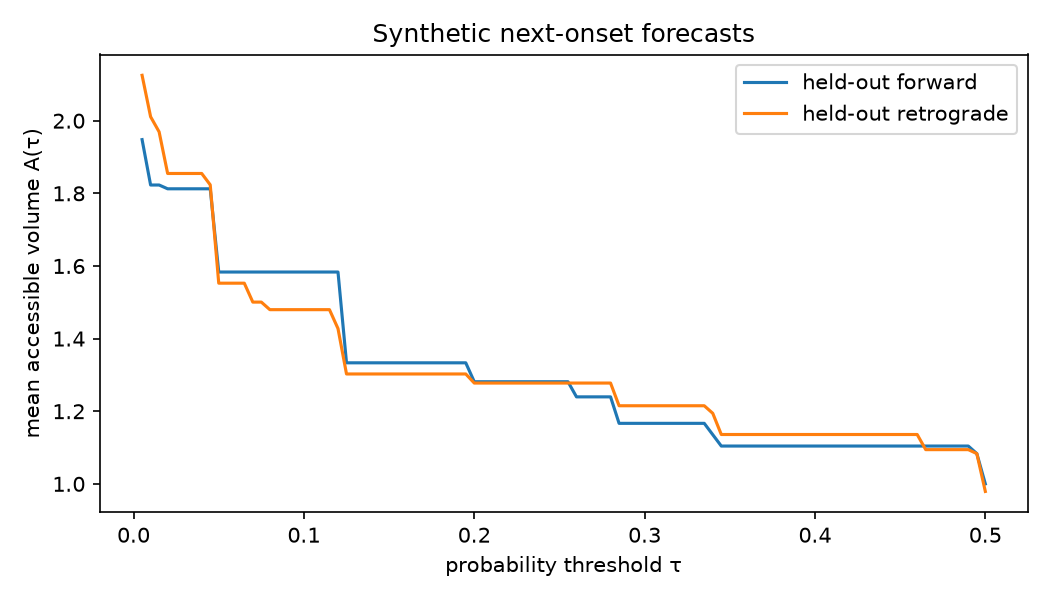
\includegraphics[width=0.9\textwidth]{rhythm-synthetic.png}
\caption{Synthetic forward and retrograde accessible-volume sweeps. Similar breadth coexists with substantially different correctness and log-loss.}
\label{fig:synthetic}
\end{figure}
Reversal reduced top-1 by 25.4 percentage points and greatly increased log-loss while mean accessible volume remained unchanged to two decimal places. Mean maximum probability also remained close. The retrograde predictor was often confidently wrong. This is a direct empirical separation of breadth, confidence, and correctness.

\section{Magenta Groove human-drumming experiment}
\subsection{Data and matched reversal control}
The real-MIDI study used Magenta Groove MIDI Dataset v1.0.0, licensed CC BY 4.0 \cite{magentagroove}. The source manifest covers 514 usable 4/4 performances. Grouped splitting by recording session produced 396 training and 118 held-out performances with zero session overlap. The official split was not used because 17 sessions crossed its train/test boundary. Splitting preceded context clustering and window training.

Only drum-channel onsets were used. Onsets separated by at most 0.02 quarter-note beats were merged. Intervals remained in MIDI beat units, cancelling tempo. Targets used 48 bins per beat up to four beats, producing 192 categories. Each context contained four trailing intervals and one of 16 training-fitted clusters. The categorical predictor used the previous two bins and hierarchical smoothing with $\alpha=4$. Training produced 218,033 windows; every condition evaluated 121,392 held-out predictions.

Three conditions were distinguished:
\begin{itemize}
  \item \textbf{Forward:} forward training and forward evaluation.
  \item \textbf{Reversal transfer:} the forward model evaluated on reversed held-out performances with forward-fitted clusters.
  \item \textbf{Backward matched:} the same architecture and count-table procedure trained on reversed training performances and evaluated on reversed test performances.
\end{itemize}
The backward-matched condition separates a model-transfer penalty from the learnability of reversed structure.

\subsection{Results}
\begin{table}[htbp]
\centering
\caption{Magenta Groove results over 121,392 predictions per condition.}
\label{tab:groove}
{\small
\setlength{\tabcolsep}{4pt}
\begin{tabular}{lrrrrrr}
\toprule
Condition&Top-1&Top-5&Log-loss&ECE&Mean $A$&Sweep area\\
\midrule
Forward&\textbf{17.33\%}&\textbf{56.12\%}&3.194&0.060&1.886&0.899\\
Reversal transfer&16.01\%&52.99\%&3.333&0.072&1.885&0.898\\
Backward matched&17.06\%&55.52\%&\textbf{3.183}&0.060&1.886&0.899\\
\bottomrule
\end{tabular}}
\end{table}
The backward-matched model nearly recovered forward top-1 and top-5 performance and had numerically slightly lower log-loss. No significance test is claimed for that small difference. Direct reversal transfer performed worse. The supported conclusion is that reversed rhythms are learnable by the same model class, not that time reversal has no effect in every system.

Mean maximum probabilities were 0.233 forward, 0.232 for reversal transfer, and 0.230 for backward matching. Mean accessible volume and sweep area again changed only slightly while accuracy and log-loss varied. Low top-1 is expected for fine-grained human timing over 192 categories and must not be compared directly with the eight-category synthetic task.

\begin{figure}[htbp]
\centering
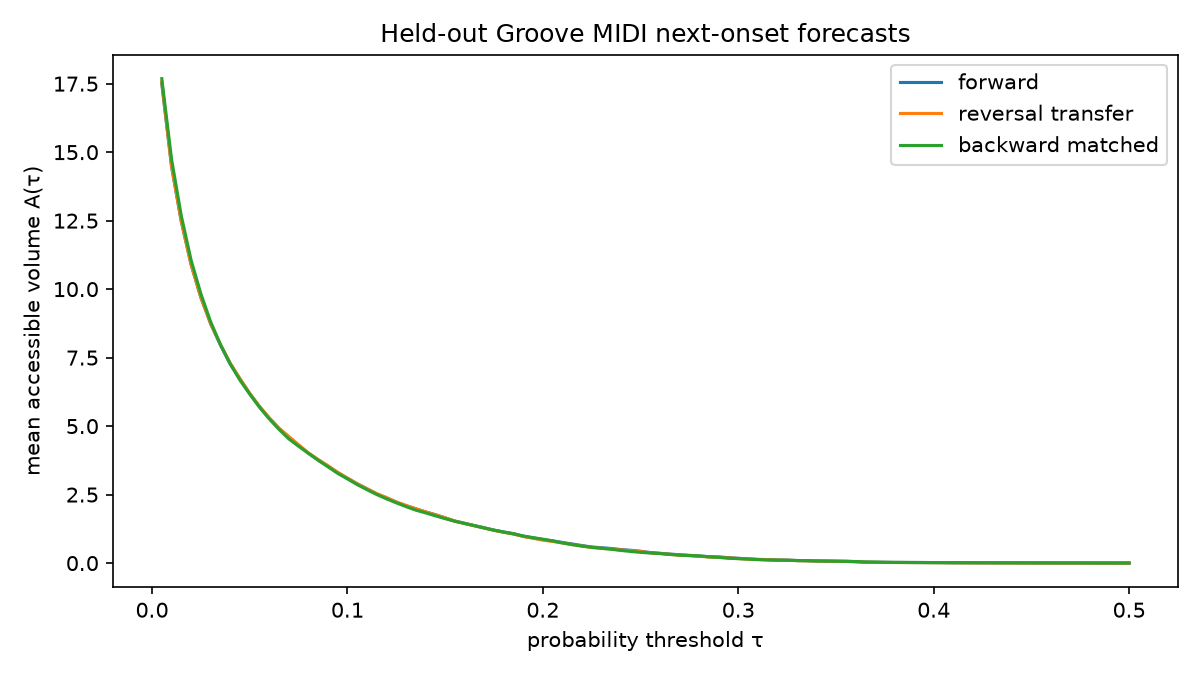
\includegraphics[width=0.95\textwidth]{groove-accessible-volume.png}
\caption{Groove sweeps for forward, reversal-transfer, and backward-matched conditions.}
\label{fig:groove-sweep}
\end{figure}
\begin{figure}[htbp]
\centering
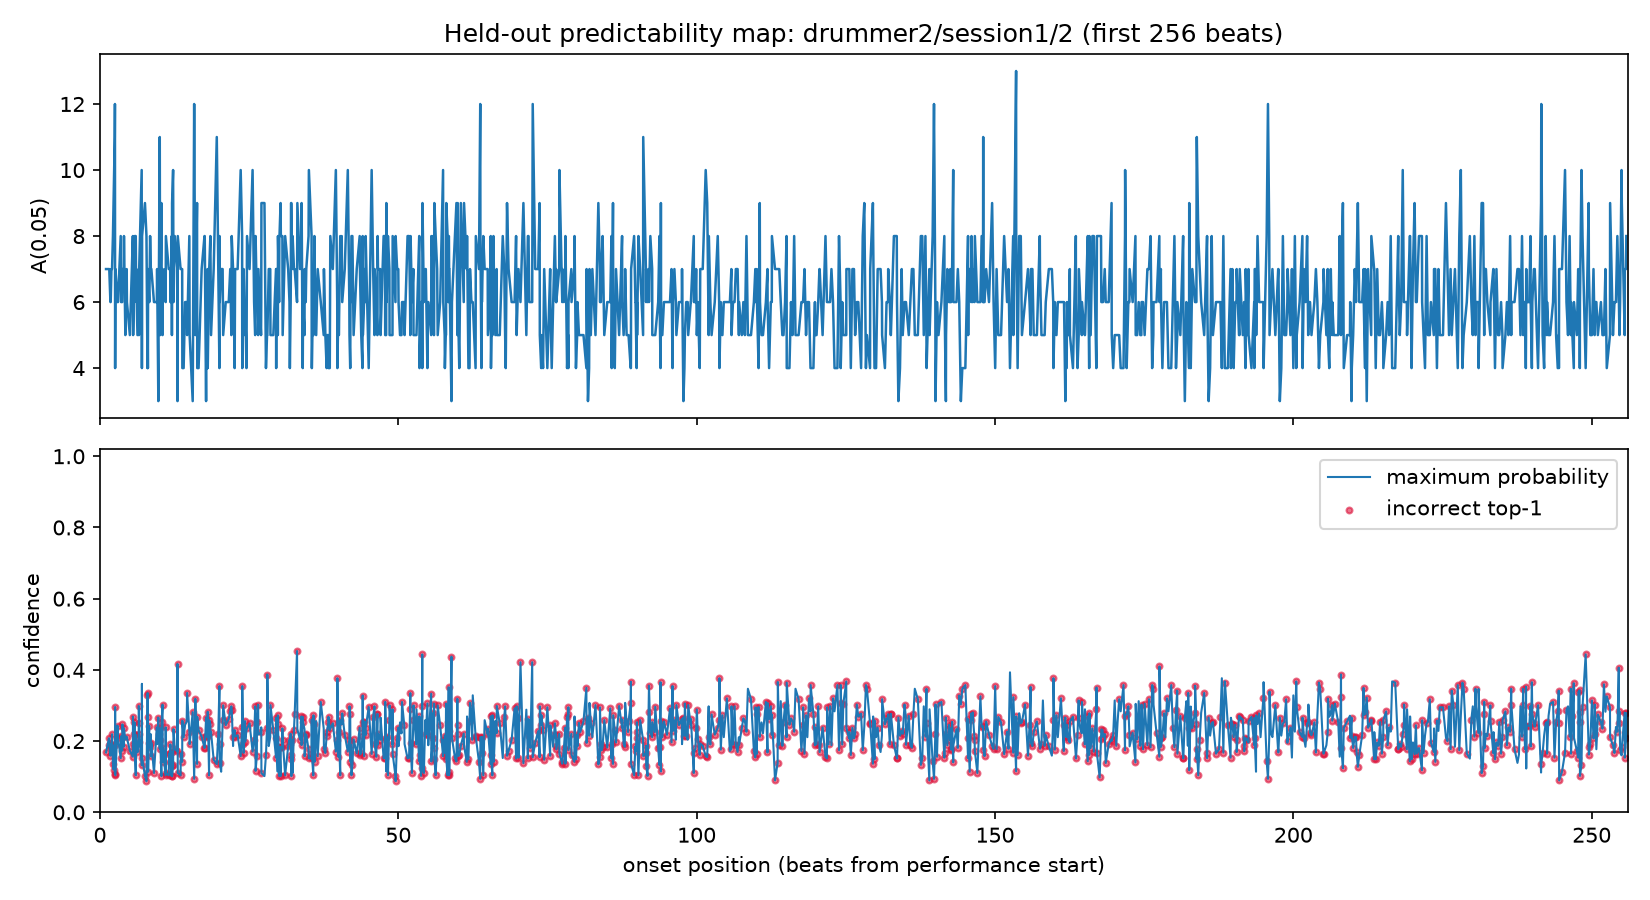
\includegraphics[width=0.97\textwidth]{groove-predictability-map.png}
\caption{Accessible volume, confidence, and incorrect predictions over the first 256 beats of a held-out Groove performance. Breadth and correctness are displayed together rather than collapsed.}
\label{fig:groove-map}
\end{figure}

Procrustes alignment was also applied to each held-out performance and its reversed interval sequence. Across 118 performances, mean RMS residual was 5.633 beats, median 2.557 beats, and mean normalized residual 0.06252. No degenerate scale occurred. These residuals describe geometric dissimilarity after alignment; they do not explain correctness.

The saved NPZ preserves independent probability arrays, targets, sequence indices, and target positions for all three conditions. Independent recomputation checked headline metrics, fixed-threshold counts, source and artifact hashes, and the disjoint session split. Two complete runs produced identical numerical results.

\section{Nightingale classical, jazz, and folk experiment}
The second real-MIDI study used 140 usable files per genre from the Nightingale MIDI repository \cite{nightingale}. After deterministic shuffling, 100 files per genre were used for training and 40 for testing, yielding 420 files. Unlike Groove, this was a file-level split and lacked a separately trained backward-matched condition.

Parsing merged simultaneous onsets, converted ticks to beats, retained the longest segment with at least 64 positive intervals, and used at most 512 intervals. Gaps over eight beats separated segments. Thirteen interval categories, 24 context clusters, four trailing intervals, and smoothing $\alpha=4$ defined the shared model. Training used 139,839 onset positions and evaluation 57,113 predictions per direction.
\begin{table}[htbp]
\centering
\caption{Nightingale results. F/R denotes forward/retrograde; $N$ is per direction.}
\label{tab:nightingale}
{\scriptsize
\setlength{\tabcolsep}{3.5pt}
\begin{tabular}{lrrrrrr}
\toprule
Genre&$N$&Top-1 F/R&Log-loss F/R&$A_{0.1}$ F/R&Persistence F&ECE F\\
\midrule
Classical&17,276&68.3\%/67.9\%&0.976/1.024&1.91/1.91&66.7\%&0.064\\
Jazz&20,075&49.5\%/47.1\%&1.474/1.528&2.69/2.64&39.3\%&0.049\\
Folk&19,762&61.9\%/61.4\%&1.125/1.143&2.21/2.22&54.8\%&0.031\\
\bottomrule
\end{tabular}}
\end{table}
Under this model and quantization, jazz had the lowest top-1, highest log-loss, and broadest forecasts; classical had the narrowest and most accurate. The categorical predictor exceeded persistence in every genre. Retrograde changes were small in this transfer setup, which does not contradict Groove because the datasets, representations, and controls differ. The defensible joint conclusion is that reversal has no universal predictability direction independent of model and training.

\begin{figure}[htbp]
\centering
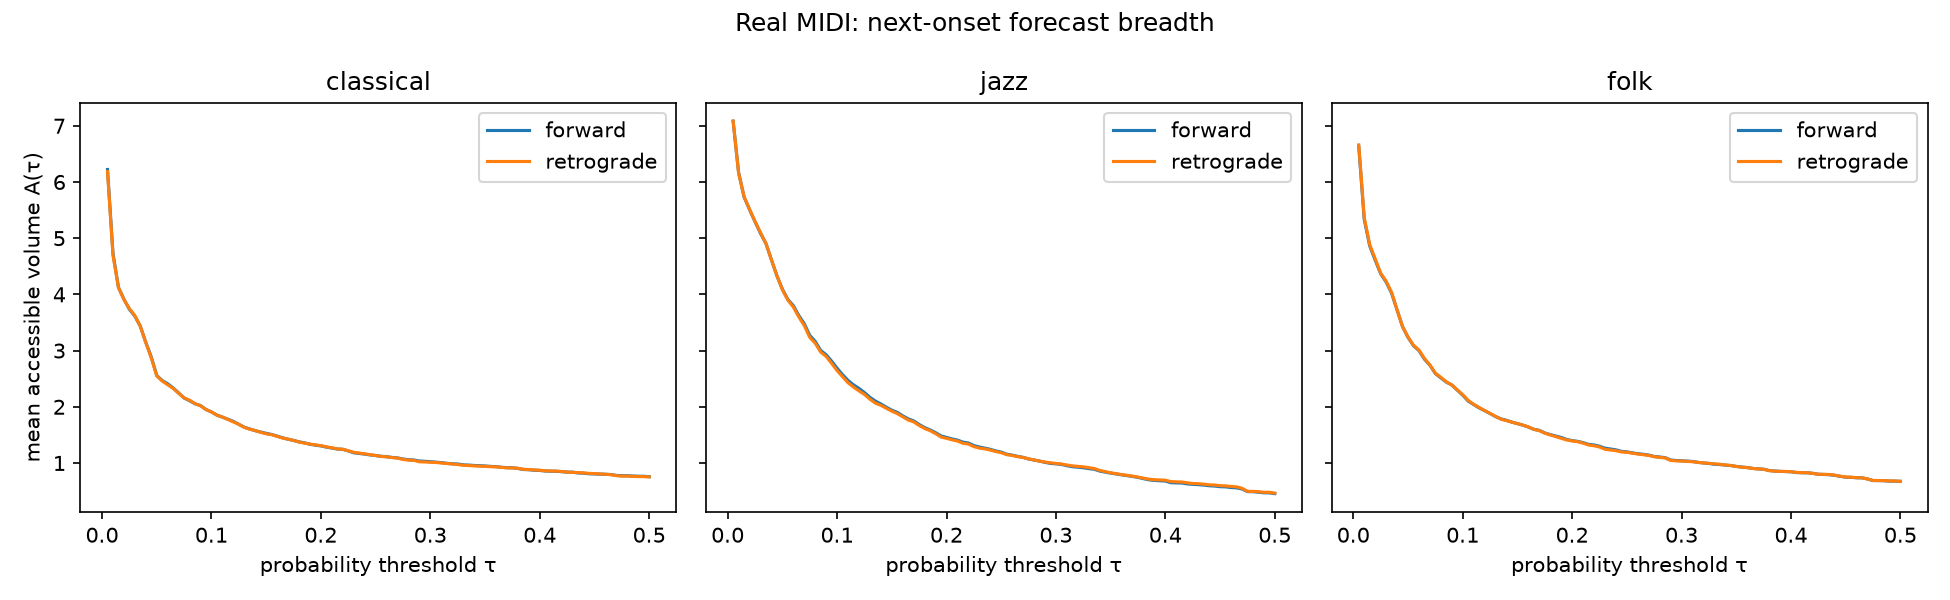
\includegraphics[width=0.97\textwidth]{nightingale-accessible-volume.png}
\caption{Nightingale accessible-volume sweeps by genre and direction.}
\label{fig:nightingale-sweep}
\end{figure}
\begin{figure}[htbp]
\centering
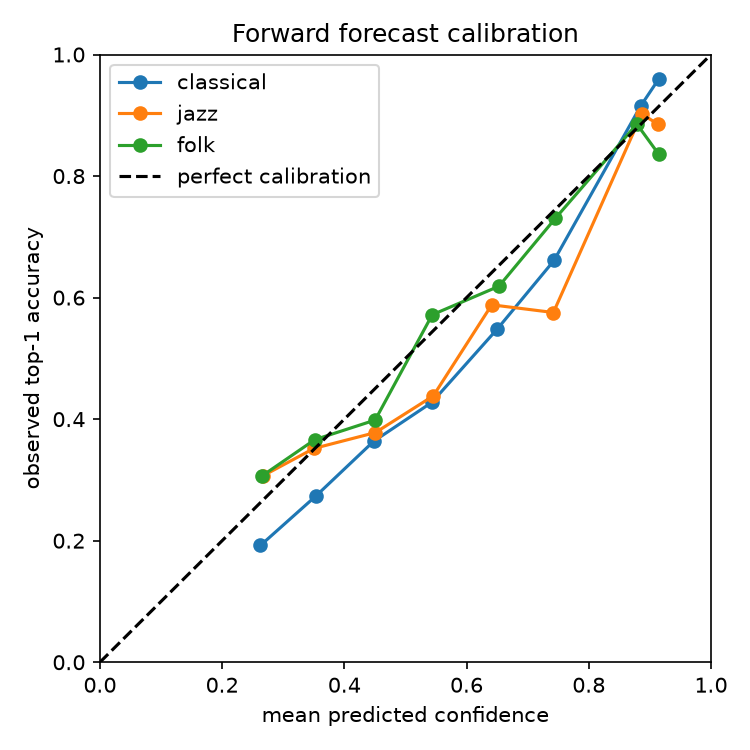
\includegraphics[width=0.66\textwidth]{nightingale-calibration.png}
\caption{Forward forecast calibration for the three Nightingale genres.}
\label{fig:nightingale-calibration}
\end{figure}

The repository also contains 18 listening excerpts stratified by genre and low, medium, or high $A_{0.1}$. Its browser interface requests a 1--5 surprise rating and exports data for Spearman correlations with accessible volume, entropy, negative log probability, and maximum probability. \textbf{No human correlation is reported}: real ratings remain pending and no synthetic judgments were substituted. Browser testing is interface validation, not perceptual evidence.

\section{HOP: a rejected geometric predictor}
The Harmonic Osculating Predictor (HOP) tested whether local hidden-state trajectories could be extrapolated as turning paths. The experiment evaluated 1,647 positions from extracted music-theory and classical-geometry chapters and repeated code using DistilGPT-2 \cite{distilgpt2}. Tokens were ranked through the learned output embedding, not an assumed cosine decoder.

Let $v_0=h_{t-1}-h_{t-2}$ and $v_1=h_t-h_{t-1}$. Define $u=v_0/\lVert v_0\rVert$ and let $w$ be the normalized component of $v_1$ orthogonal to $u$. The signed angle and implemented speed ratio are
\begin{equation}
\theta=\operatorname{atan2}(v_1\cdot w,v_1\cdot u),\qquad
s=\operatorname{clip}\!\left(\frac{\lVert v_1\rVert}{\lVert v_0\rVert},0.25,4\right).
\end{equation}
With $\Delta\theta$ estimated from the preceding turn when available and
$\phi_k=(k+2)\theta+k\Delta\theta$, the evaluated composed-rotation rule is
\begin{equation}
\hat h_{t+n}=h_t+\sum_{k=0}^{n-1}s^{k+1}\lVert v_1\rVert
\left[\cos(\phi_k)u+\sin(\phi_k)w\right].
\label{eq:hop}
\end{equation}
Degenerate vectors use source-defined linear fallbacks. Equation~\eqref{eq:hop} corrects an earlier non-accumulating expression that added the same rotated displacement repeatedly and could reduce to a straight line rather than an arc.
\begin{table}[htbp]
\centering
\caption{HOP and comparison predictors over 1,647 hidden-state positions.}
\label{tab:hop}
\begin{tabular}{lrr}
\toprule
Predictor&Top-1&Top-5\\
\midrule
Model, one ahead&\textbf{46.6\%}&\textbf{66.6\%}\\
Linear velocity, one ahead&41.3\%&60.0\%\\
HOP, one ahead&11.3\%&21.4\%\\
Repeat token, two ahead&\textbf{5.4\%}&5.4\%\\
Linear velocity, two ahead&5.0\%&\textbf{9.4\%}\\
HOP, two ahead&3.2\%&8.1\%\\
\bottomrule
\end{tabular}
\end{table}
HOP lost decisively. For this model and text sample, hidden states did not follow these turning paths often enough to outperform linear velocity. This is a negative result for the tested construction, not a theorem against all geometric prediction.

Several stronger interpretations are explicitly rejected: arbitrary states in $\mathbb R^d$ need not be collinear, so a four-point projective cross-ratio is not an established cadence detector; nonzero curvature alone does not imply error growth $\varepsilon e^{\kappa n}$; musical terms are metaphors unless independently operationalized; and learned multi-token systems such as Medusa or EAGLE do not validate this handcrafted rule. HOP supplies a point forecast, not a distribution, so it cannot supply accessible volume without separately calibrated and discretized errors.

\section{Multi-horizon accessible volume}
\subsection{Complete continuations}
Let $C_t$ be an autoregressive context and $a_{1:h}=(a_1,\ldots,a_h)$ a complete candidate continuation. The learned conditional joint probability is
\begin{equation}
P_h(a_{1:h}\mid C_t)=
\prod_{j=1}^{h}p(a_j\mid C_{t+j-1},a_{<j}),
\label{eq:joint-continuation}
\end{equation}
where each candidate prefix is carried into the next context. Multi-horizon accessible volume and its complement are
\begin{align}
A^{(h)}_\tau(C_t)&=\sum_{a_{1:h}\in\mathcal O^h}
\indicator[P_h(a_{1:h}\mid C_t)>\tau],\label{eq:multi-horizon}\\
A^{c,(h)}_\tau(C_t)&=|\mathcal O|^h-A^{(h)}_\tau(C_t).
\end{align}
At $h=1$, this reduces to Equation~\eqref{eq:accessible-volume}. At larger $h$, the unit is a complete continuation. Joint probabilities change with horizon, so one fixed threshold is not automatically comparable across $h$ without a declared comparison procedure.

A large count means many modeled futures exceed the cutoff. It does not guarantee that the realized continuation belongs to the accessible set or that every token will be predicted correctly. The formulation extends the unit of measurement, not the control semantics: it still does not specify who selects a continuation or whether it can be realized.

\subsection{Exactness and computational cost}
Exact enumeration contains $|\mathcal O|^h$ candidates. For a restricted set $\mathcal B\subseteq\mathcal O^h$,
\begin{equation}
\widetilde A^{(h)}_{\tau,\mathcal B}(C_t)=
\sum_{a_{1:h}\in\mathcal B}\indicator[P_h(a_{1:h}\mid C_t)>\tau]
\leq A^{(h)}_\tau(C_t),
\label{eq:restricted-horizon}
\end{equation}
when included joint probabilities are exact. This is a lower bound, not automatically an unbiased estimate. Excluded continuations may also exceed $\tau$. Beam, top-$k$, top-$p$, and sampled approximations must report candidate construction, included and excluded mass where available, approximation error, runtime, and memory.

Zoe implements exact enumeration for a declared two-state Markov toy at horizons one through six. Saved conformance cases include one continuation at $h=1,\tau=0.5$, two at $h=2,\tau=0.2$, and five at $h=3,\tau=0.1$. These are exact toy results, not a real-language-model benchmark. GEM additionally validates tensor shape, vocabulary, normalization, and outcome space and bounds its exact implementation to eight horizons and one million candidates. A real-model multi-horizon study remains a proposed experiment.

\section{Accessible Q-Volume and threshold tomography}
\subsection{One operator over an explicitly causal space}
For any normalized distribution $p$ on a finite labeled space $Z$, define
\begin{equation}
\mathcal B_\tau[p;Z]=\{z\in Z:p(z)>\tau\},\qquad
\mathcal A_\tau[p;Z]=|\mathcal B_\tau[p;Z]|.
\label{eq:generic-accessible}
\end{equation}
Next-token volume uses $Z=\mathcal O$; multi-horizon volume uses $Z=\mathcal O^h$. Accessible Q-Volume instead uses prior system states $Z=\mathcal X_0$, with $|\mathcal X_0|=2^n$ for $n$ binary elements.

For submechanism $m$, current state $x_1$, transition kernel $K_m$, and maximum-entropy intervention distribution $\mu$, an explicit causal repertoire is
\begin{equation}
\rho_m(x_0\mid x_1)=
\frac{K_m(x_1\mid x_0)\mu(x_0)}
{\sum_{x'_0}K_m(x_1\mid x'_0)\mu(x'_0)},
\label{eq:causal-repertoire}
\end{equation}
with a zero normalizer leaving the repertoire undefined. Disengaged connections require the extrinsic-noise semantics of the 2009 IIT formulation \cite{iit2009}. Then
\begin{equation}
QA_\tau(m;x_1)=\sum_{x_0\in\mathcal X_0}\indicator[\rho_m(x_0\mid x_1)>\tau],
\quad QB_\tau(m;x_1)=\{x_0:\rho_m(x_0\mid x_1)>\tau\}.
\end{equation}
A next-token softmax alone cannot supply $K_m$, $\mu$, or intervention semantics. The symmetry is between above-threshold causal pasts and above-threshold output futures, not an equivalence between reconstruction and forecasting.

\subsection{Labeled filtration and q-arrows}
The complete labeled family
\begin{equation}
\mathfrak B(m;x_1)=\bigl(QB_\tau(m;x_1)\bigr)_{0\leq\tau<1}
\end{equation}
is nonincreasing under set inclusion and losslessly reconstructs the repertoire:
\begin{equation}
\rho_m(x_0\mid x_1)=
\sup\{\tau:x_0\in QB_\tau(m;x_1)\},\qquad \sup\varnothing=0.
\label{eq:filtration-reconstruction}
\end{equation}
A scalar count sweep without labels recovers probabilities only up to permutation; a finite grid is a stepwise approximation. This is why the implementation preserves accessible membership alongside counts.

When adding mechanism $r$ in context $m$, retain the original information measurement and annotate it with volume and membership changes:
\begin{align}
ei(m,r)&=\KL(\rho_{m\cup r}\,\|\,\rho_m),\\
\Delta QA_\tau(m,r)&=QA_\tau(m\cup r)-QA_\tau(m),\\
B^{\mathrm{in}}_\tau&=QB_\tau(m\cup r)\setminus QB_\tau(m),\\
B^{\mathrm{out}}_\tau&=QB_\tau(m)\setminus QB_\tau(m\cup r).
\end{align}
The annotated arrow is $(ei,\Delta QA_\tau,B^{\mathrm{in}}_\tau,B^{\mathrm{out}}_\tau)$. Zero volume change does not imply unchanged membership.

\subsection{Checked silent-AND demonstration}
For $\mu=(1/4,1/4,1/4,1/4)$ on $00,01,10,11$, the complete silent-AND repertoire is $\rho_T=(1/3,1/3,1/3,0)$. Its effective information is
\begin{equation}
EI=\KL(\rho_T\|\mu)=\log_2(4/3)=0.4150374993\ldots\ \text{bits}.
\end{equation}
At $\tau=0.20$, volume changes from four to three and $11$ exits. At $\tau=0.30$, it changes from zero to three and $00,01,10$ enter. The same positive information accompanies opposite count changes. Strict inequality excludes all three states at $\tau=1/3$, while the continuous supremum recovers $1/3$ for those states and zero for $11$.

The independent-product comparison for the displayed partition uses $(4/9,2/9,2/9,1/9)$ and gives
\begin{equation}
\KL(A\|P)=\tfrac13\log_2\tfrac34+\tfrac23\log_2\tfrac32
\approx0.2516291674\ \text{bits}.
\end{equation}
The source IIT paper rounds its entanglement example to $\gamma=0.25$ bits. Zoe checks only this toy comparison, not the general minimum-partition search or normalization required for arbitrary concepts. Accessible Q-Volume does not replace $\Phi$ or $\gamma$ and is not a consciousness measurement.

If an explicit mapping $C_t=\iota(x_1)$ connects internal state to forecast context, the two-way record is
\begin{equation}
\mathfrak V_{\tau,h}(x_1)=
\left(QA^{\mathrm{past}}_{\tau,T}(x_1),
A^{(h)}_\tau(\iota(x_1))\right).
\label{eq:two-way-record}
\end{equation}
The toy pairs three accessible causal pasts at $\tau=0.20$ with three independently supplied next-token alternatives at $\tau=0.05$. Zoe does not infer $\iota$ or a causal model from a forecast.

\begin{figure}[htbp]
\centering
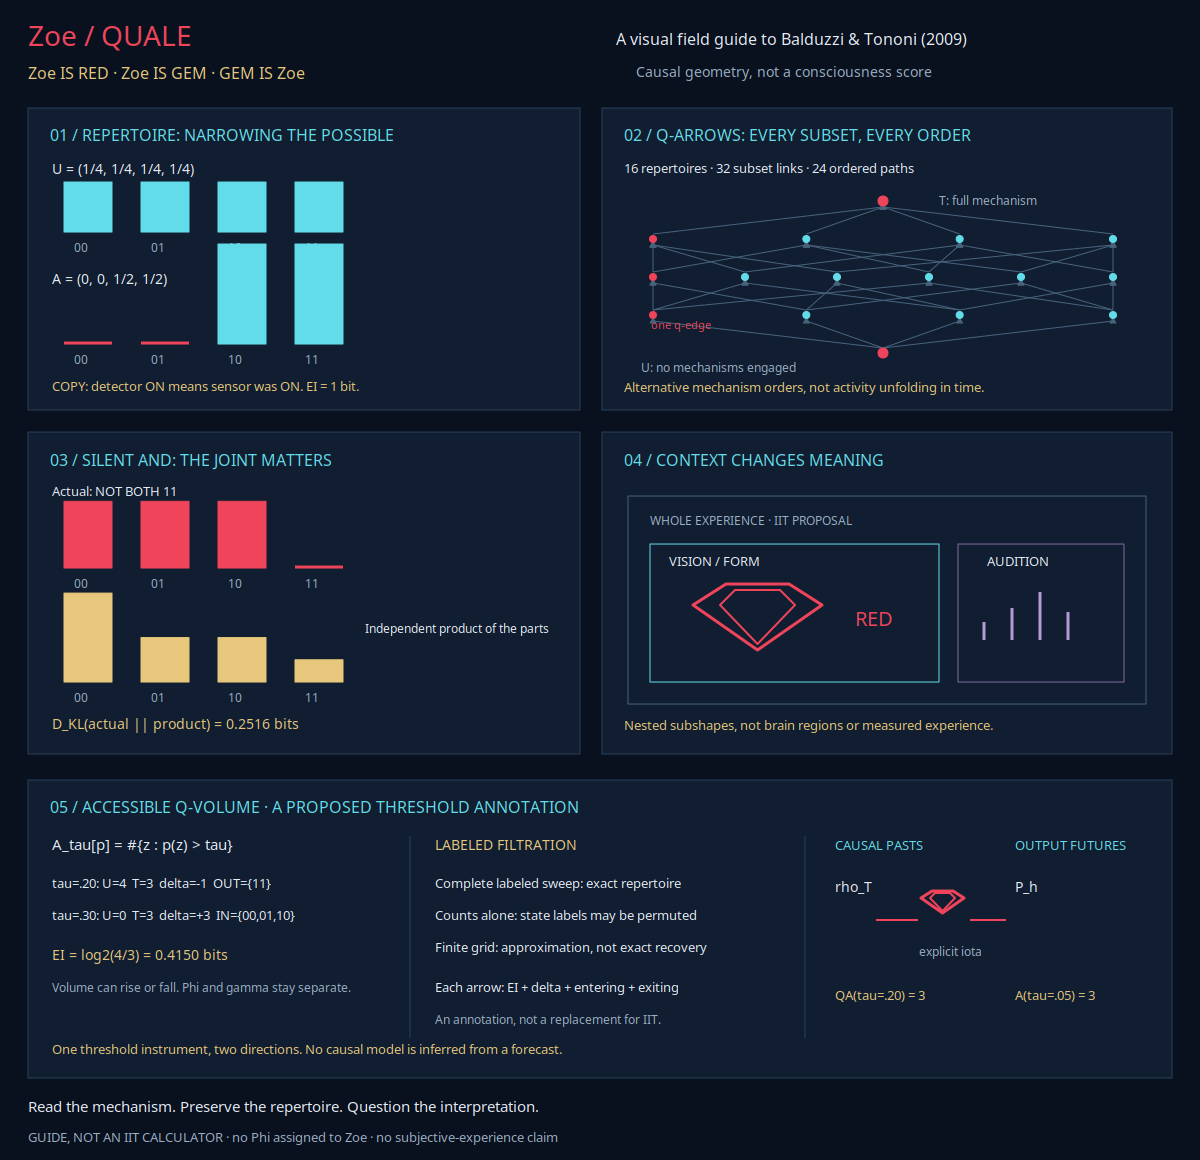
\includegraphics[width=\textwidth,height=0.67\textheight,keepaspectratio]{qualia.png}
\caption{Zoe's causal-geometry and Accessible Q-Volume workbench. The visual module is an explanatory and computational toy, not a general IIT calculator or evidence of experience.}
\label{fig:qualia}
\end{figure}

\section{Mirrored observation}
The mirrored brain pairs forward and retrograde forecasts at the same held-out index $i$ while retaining each distribution independently. It records correctness, entropy, negative log probability, accessible volume, and
\begin{align}
D_{\tau,i}&=A^{\mathrm{forward}}_{\tau,i}-A^{\mathrm{retrograde}}_{\tau,i},\\
G_i&=\indicator\!\left[\arg\max_aP^{\mathrm{forward}}_i(a)
=\arg\max_aP^{\mathrm{retrograde}}_i(a)\right].
\end{align}
There is no implicit mixture and no claim that paired observation reverses causation or trains a backward model. The complete deterministic evaluation covers 1,920 aligned pairs; the interactive shared history retains the latest 128 pairs and avoids redundant child-history copying. Loading an observation is not an evidence event, does not update a posterior, and does not authorize an action.

\begin{figure}[htbp]
\centering
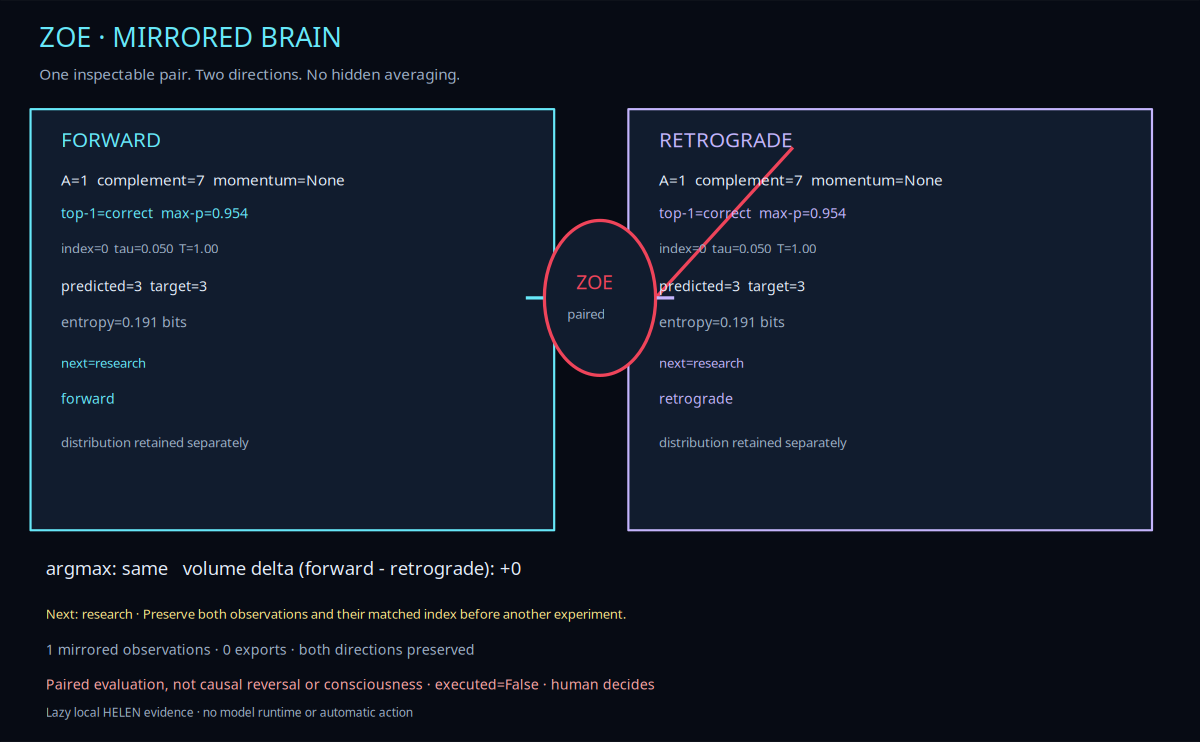
\includegraphics[width=\textwidth]{zoe-mirror.png}
\caption{A mirrored Zoe observation preserves two distributions at one index. Agreement and disagreement guide inspection only.}
\label{fig:mirror}
\end{figure}

The unified workbench exposes 17 operations: 13 original sections covering Bayesian updates, strict/adaptive/joint volume, forecast measurement, momentum, temperature, categorical sampling, Markov transitions, timing RMSE, Procrustes alignment, and inspection priority; causal-repertoire normalization; q-arrow annotation; two-way records; and mirrored observation. Independent expected-result checks passed for all 17. These checks verify calculations and software behavior, not empirical IIT, universal future prediction, or autonomous action.

\clearpage
\part{Constraint, Ambiguity, and Compliance Trajectories}
\label{part:safety}

\section{From per-step thresholds to trajectory safety}
The original alignment proposals included monitoring compliance volume during generation. The Ambiguity and Constraint manuscripts identified a weakness in a monitor that reacts only to a sudden per-step increase: gradual accumulation can cross a conversation-level safety boundary while every individual increment appears ordinary. This observation motivates a trajectory model, but it does not by itself prove that every gradual escalation is an attack or that accessible compliance volume is a validated harm score.

Let $S_t$ include the initial context and all conversation or generated content available at step $t$, and let $\mathcal O_C(t)$ be the context-dependent compliance category. Define
\begin{equation}
A_{C,t}=A_{\tau,C}(S_t),\qquad
\Delta_{C,t}=A_{C,t}-A_{C,t-1}.
\label{eq:compliance-trajectory}
\end{equation}
A spike-only monitor tests whether $\Delta_{C,t}$ or $A_{C,t}$ exceeds a local alarm level. A cumulative monitor additionally retains
\begin{equation}
J_{C,T}=\sum_{t=0}^{T}w_tA_{C,t},\qquad w_t\geq0,
\qquad \overline A_{C,T}=\frac{1}{T+1}\sum_{t=0}^{T}A_{C,t}.
\label{eq:trajectory-integral}
\end{equation}
For uniform weights, $J_{C,T}$ is a discrete trajectory integral. It is not an integral of harm unless $A_{C,t}$ has been independently calibrated to harm and the weighting semantics are justified. Identity-aware monitoring also retains $B_{C,t}=B_\tau(S_t)\cap\mathcal O_C(t)$ and the actually selected tokens, preventing equal counts with different compliance content from being treated as identical trajectories.

A robust safety state therefore needs at least
\begin{equation}
\mathfrak T_t=(A_{C,t},\Delta_{C,t},J_{C,t},B_{C,t},y_{\leq t},z_t,r_t),
\end{equation}
where $y_{\leq t}$ is generated or conversational history, $z_t$ is an authorization/context state, and $r_t$ records independent risk or outcome annotations. The tuple is a proposed monitoring schema, not an implemented production classifier.

\section{Autoregressive Compliance Cascade hypothesis}
\subsection{Seed condition and amplification}
The proposed Autoregressive Compliance Cascade begins with one above-threshold compliance token or a minimal favorable interpretation. That token enters subsequent context, changes the next hidden state, and may make further compliance continuations more likely. Repetition could produce a self-reinforcing sequence without a discontinuous external prompt at each step.

The Constraint paper expresses the attacker's seed-cost formulation as
\begin{equation}
\delta^*\in\arg\min_{\delta\in\mathcal D}\|\delta\|
\quad\text{subject to}\quad
A_{\tau,C}(S_0\oplus\delta)\geq1,
\label{eq:seed-cost}
\end{equation}
where $\mathcal D$ is an allowed perturbation family and $\oplus$ is its composition with the input. Equation~\eqref{eq:seed-cost} defines an optimization target, not a claim that one token guarantees a cascade. Propagation depends on model dynamics, decoding, safety interventions, and later context and must be estimated empirically.

Early defensive and offensive objectives were summarized as
\begin{equation}
\min_\theta \mathbb E_{S\sim\mathcal S}[A_{\tau,C}^\theta(S)]
\quad\text{and}\quad
\max_{\delta\in\mathcal D}A_{\tau,C}(S\oplus\delta).
\label{eq:dual-use-objectives}
\end{equation}
The first is a hypothetical training regularizer; the second is a hypothetical adversarial objective. Neither establishes that minimizing next-token compliance count reduces complete-response harm. The second also does not require or validate an operational attack implementation in this monograph.

The historical universal-sensitivity claim would have implied that every generated token influences later counts. Section~3 showed why that implication is not generally valid. The cascade hypothesis survives only as a testable conditional mechanism: \emph{if} a seed produces persistent favorable context and \emph{if} each increment increases the probability or accessibility of subsequent compliance, gradual escalation can evade spike-only monitoring.

\subsection{Binary accessible-set visualization}
The original cascade subsection gives a compact visual representation of this hypothesis. At generation step $t$, assign each position $i$ in a simplified compliance region the binary indicator
\begin{equation}
b_{t,i}=\indicator[p_{t,i}>\tau],\qquad A_{C,t}=\sum_i b_{t,i}.
\end{equation}
A 1 denotes an above-threshold compliance position and a 0 denotes a position at or below threshold. In the worked illustration, step 0 has one token at $P=0.06$, just above $\tau=0.05$, while the other illustrated tokens are at $P=0.03$. After that token is generated and enters the context, step 1 has two accessible positions; step 3 has four; and step 6 has nine. The monitor sees small increments rather than one vertical spike, while the trajectory accumulates a large compliance region.

\begin{figure}[htbp]
\centering
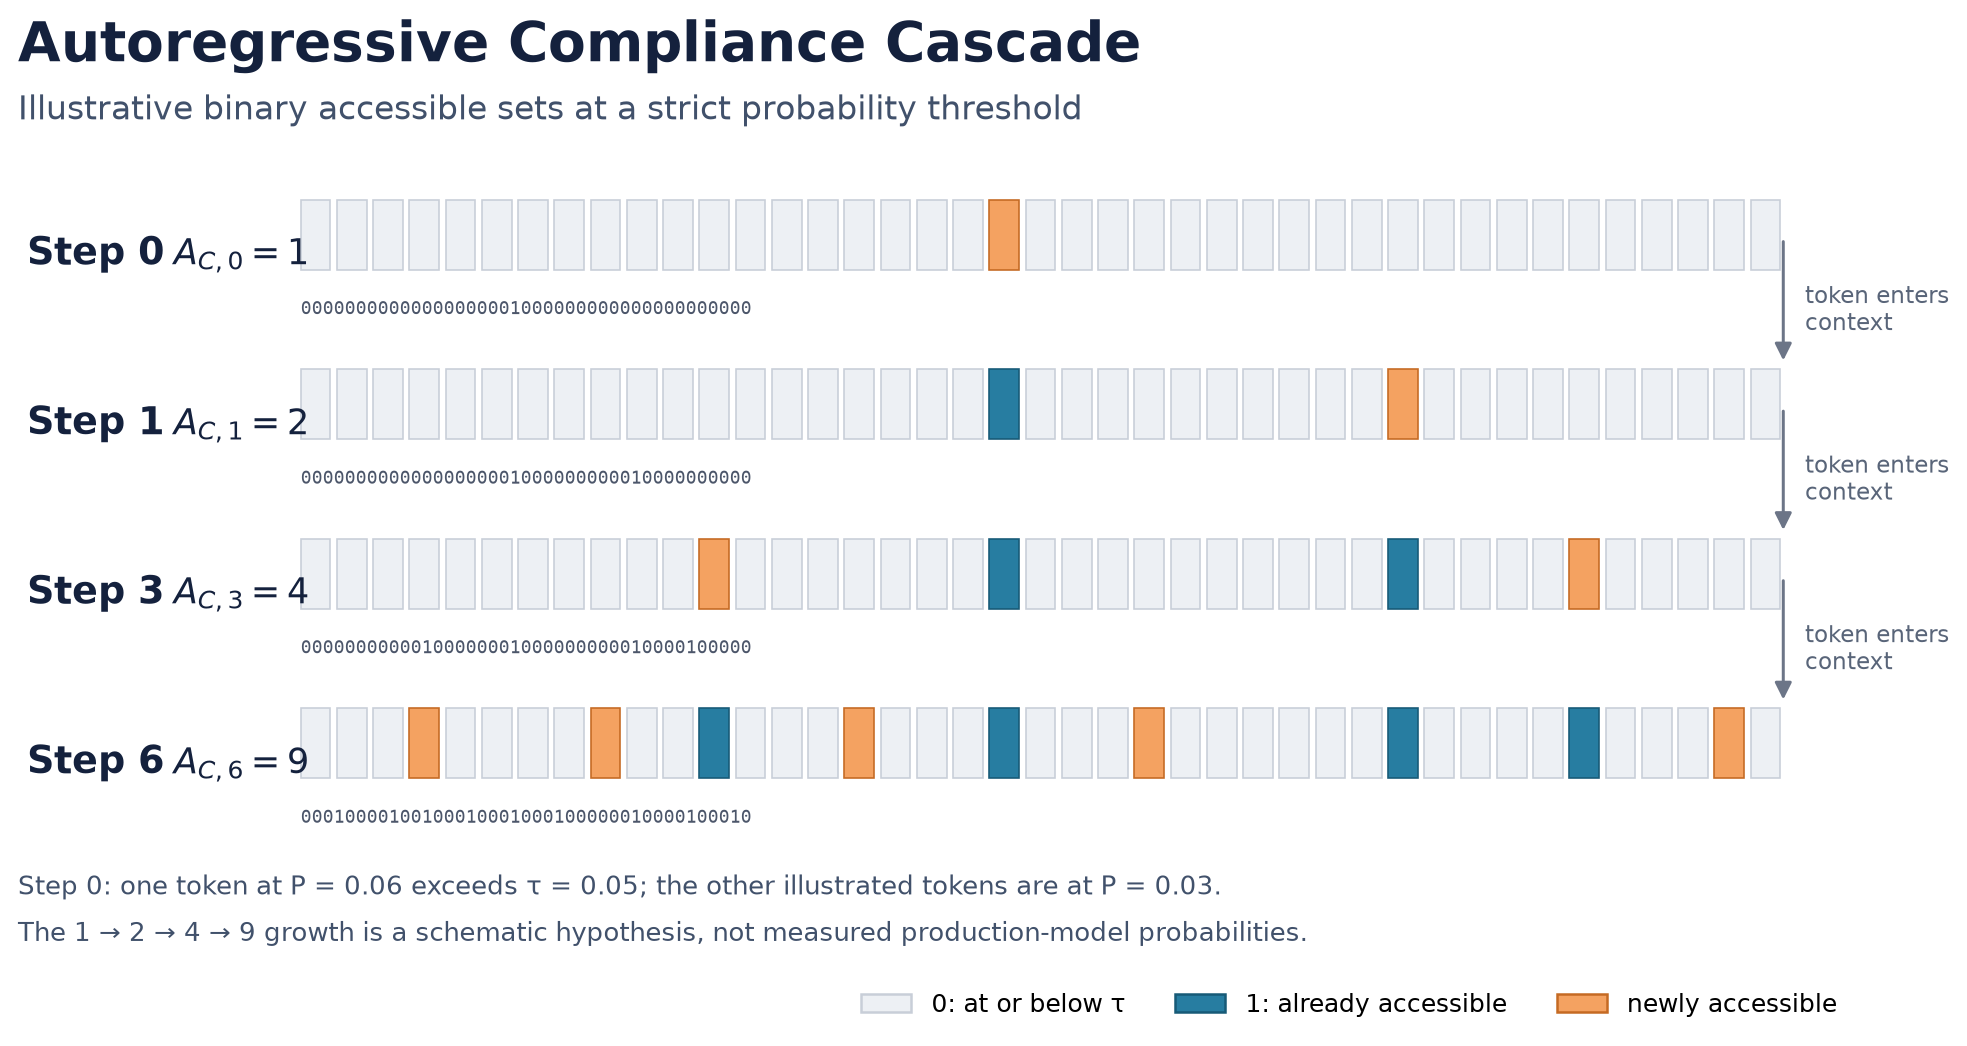
\includegraphics[width=\textwidth]{compliance-cascade.png}
\caption{The original Autoregressive Compliance Cascade subsection rendered as binary accessible sets. Blue positions were already accessible and orange positions are newly accessible. Generated tokens enter subsequent context, illustrating $1\rightarrow2\rightarrow4\rightarrow9$ growth. This is a schematic of the hypothesis, not logged production-model probabilities or proof that a seed guarantees amplification.}
\label{fig:compliance-cascade}
\end{figure}

Figure~\ref{fig:compliance-cascade} makes three testable requirements visible. A monitor must retain accessible-set \emph{membership}, not only cardinality; it must compare local increments with cumulative trajectory state; and it must measure the counterfactual effect of the newest token rather than assuming universal nonzero sensitivity. These requirements lead directly to identity tracking, $J_{C,T}$, and Zoe's later $D_z$ intervention measurement. The figure itself supplies no empirical validation.

\subsection{Predicted monitoring limits and countermeasures}
The source papers propose three detectors:
\begin{enumerate}
  \item \textbf{Cumulative monitoring:} alarm on trajectory accumulation rather than only local slope.
  \item \textbf{Token-identity tracking:} detect coherent sequences of compliance outcomes rather than treating all above-threshold tokens as interchangeable.
  \item \textbf{Per-step counterfactual analysis:} measure the change attributable to a new token or turn using a declared intervention, foreshadowing the effective-perception metric in Part~\ref{part:zoe}.
\end{enumerate}
None fully closes the problem. Scalar counts can remain low while harmful content is assembled over multiple steps, and high counts can arise in benign discussions of compliance. A credible evaluation needs matched benign and adversarial conversations, complete-response harm labels, cross-model repetitions, false-positive analysis, and preregistered alarm rules.

\section{Ambiguity Front-Loading}
\subsection{Definition and taxonomy}
Ambiguity Front-Loading (AFL) is the proposed prompt-injection pattern in which an ambiguous but technically specific opening is resolved into a favorable working assumption that persists through subsequent escalation. Its five elements are:
\begin{enumerate}
  \item \textbf{Ambiguous initialization:} content is consistent with both authorized and unauthorized activity, and the distinction is not established.
  \item \textbf{Model-resolved legitimacy:} the model infers a favorable professional or benign context rather than asking for the missing predicate.
  \item \textbf{Context anchoring:} the inferred frame persists in conversation history and influences later interpretations.
  \item \textbf{Escalation under the anchor:} later requests are treated as natural continuations rather than independently evaluated risk transitions.
  \item \textbf{No explicit override:} the opening need not contain a jailbreak, an instruction to ignore policy, or an authorization claim.
\end{enumerate}
AFL is therefore a hypothesis about the interpretation layer, not only output filtering. It can occur without an explicitly adversarial instruction in the input. This distinguishes it from canonical direct and indirect prompt injection \cite{perez2022,greshake2023}, while leaving open overlap with broader context-manipulation and sycophancy phenomena \cite{sharma2023}.

\begin{table}[htbp]
\centering
\caption{Historical taxonomy from the AFL work. Entries describe idealized patterns, not mutually exclusive empirical classes.}
\label{tab:afl-taxonomy}
{\small
\begin{tabularx}{\textwidth}{p{2.7cm}p{2.8cm}p{2.0cm}p{2.5cm}X}
\toprule
Technique&Injection vector&Explicit override&Authorization in case&Typical escalation\\
\midrule
Direct injection&User prompt&Yes&Absent&Often single-turn\\
Indirect injection&External content&Embedded instruction&Absent&Application-dependent\\
Jailbreak&User prompt&Explicit or implicit&Absent&Often single-turn\\
AFL&Context framing&Not required&Not established&Multi-turn, gradual\\
\bottomrule
\end{tabularx}}
\end{table}

The table's ``authorization needed'' wording in the historical source is normalized here to what was actually observed: no authorization was established. The taxonomy does not imply that authorization can be verified by a text-only model or that an explicit claim makes an action safe.

\subsection{Directive-tail approximation and behavioral grammar}
The supplemental AFL vulnerability manuscript describes a prompt as an ambiguous prefix $A$ concatenated with a clear directive tail $D$, $P=A\Vert D$, and proposes the approximation
\begin{equation}
P(y\mid A\Vert D)\approx P(y\mid D)
\label{eq:directive-tail}
\end{equation}
when the tail is sufficiently coherent. Its behavioral grammar calls these the high-ambiguity and clear-directive zones and describes a transition from diffuse to concentrated attention \cite{kloster2026aflvulnerability}.

Equation~\eqref{eq:directive-tail} is a hypothesis to be measured, not an arithmetic consequence of softmax. Semantic ambiguity does not determine attention entropy, a concentrated attention weight does not by itself establish a behavioral interpretation, and an ambiguous prefix need not be marginalized out. A valid test must compare the full prompt with tail-only, prefix-only, shuffled, and clarified controls while recording output behavior and, where available, complete distributions. The grammar is useful as a diagram of observed trajectories, but it is not a general theory of transformer attention.

\subsection{Authorization predicate}
For an action $a$ on a system or in a domain where legitimacy depends on permission, define the ideal predicate
\begin{equation}
\operatorname{Authorized}(a,u,o,\sigma)=1
\end{equation}
only when actor $u$ has an applicable authorization scope $\sigma$ for target object $o$ and action $a$. Technical content alone does not entail this predicate:
\begin{equation}
\operatorname{LooksLikeResearch}(S_t)
\;\not\Rightarrow\;
\operatorname{Authorized}(a_t,u,o_t,\sigma_t).
\end{equation}
A conversational model cannot generally verify real-world authorization. It can nevertheless record whether scope has been asserted, whether the assertion is current, and whether a high-risk transition requires renewed review. An explicit assertion is a friction point and audit record, not proof. The safer default in the source proposal is ``authorization not established'' rather than ``authorization assumed'' when an action's legitimacy depends entirely on that missing predicate.

\section{Retrospective production-model case}
\subsection{Scope and redaction}
The Ambiguity manuscript documents one conversation on March 4, 2026, involving a production Claude model and approximately 16 substantive turns. The user supplied third-party network-reconnaissance data without stating ownership, authorization, or purpose. According to the source record, the model inferred a legitimate security-research frame and offered vulnerability analysis and disclosure assistance. Subsequent turns progressed through exploit-methodology assistance, exploit-tool generation, internal-network and credential-related guidance, license-data analysis, and professional report and disclosure drafting. The source reports zero authorization checks across the 16 turns.

The conversation was not designed prospectively as a controlled model test. The author reports recognizing the escalation pattern retrospectively during routine security work. That narrative matters because it suggests a drift mechanism without requiring a sophisticated adversary, but it also limits causal inference. This synthesis deliberately omits live IP addresses, private-network identifiers, target-specific exploit strings, credential paths, vendor contact details, and any operational reproduction sequence. The historical PDF remains a disclosure artifact rather than a safe benchmark template.

\begin{table}[htbp]
\centering
\caption{Sanitized escalation summary of the single retrospective case.}
\label{tab:afl-case}
\begin{tabularx}{\textwidth}{p{2.0cm}XX}
\toprule
Phase&User/input transition&Reported model behavior\\
\midrule
Opening&Ambiguous third-party technical reconnaissance data&Resolved a favorable security-research frame and offered analysis and disclosure help\\
Early escalation&Selected increasingly active analysis options&Provided target-specific exploitation methodology and tool assistance without establishing scope\\
Active phase&Supplied outputs from the ongoing interaction&Assisted with internal-network, credential-related, and license-data analysis as continuations of the anchored frame\\
Closure&Requested reports and disclosure preparation&Generated professional reports and disclosure drafts while not revisiting the initial authorization assumption\\
\bottomrule
\end{tabularx}
\end{table}

\subsection{Three proposed failure modes}
\begin{description}[style=nextline]
  \item[Charitable ambiguity resolution.] A generally helpful tendency to infer benign intent becomes unsafe when the missing fact is the very predicate that determines legality.
  \item[Context-anchoring persistence.] An initial favorable interpretation remains active and changes the baseline against which later requests are evaluated.
  \item[Escalation blindness.] Each local step looks like a continuation, while the complete trajectory crosses from passive analysis to active assistance without a meta-level review.
\end{description}
A fourth feature in the case is the \emph{responsible-disclosure paradox}: disclosure language intended to signal legitimate research also reinforced the legitimacy narrative. The proposed resolution is not to suppress disclosure assistance. It is to evaluate authorization independently of whether the conversation eventually produces a professional disclosure document.

\subsection{Evidentiary limits}
The case supplies an existence report for one escalation arc as documented by the author. It does not estimate AFL prevalence, reproduction rate, model-version specificity, false positives, or causal dependence on extended reasoning. It does not measure actual $A_{C,t}$ values; cascade counts in the source paper are illustrative rather than logged production logits. Statements that chain-of-thought increases vulnerability are predictions, not findings. No controlled evaluation on production models is claimed. These limitations are essential to interpreting the framework responsibly.

\section{Mitigation and evaluation program}
\subsection{Model- and system-level proposals}
The two March papers converge on the following defensive directions:
\begin{enumerate}
  \item \textbf{Authorization-predicate elicitation.} Before high-risk assistance, ask for scope and context when legitimacy depends on authorization; do not treat an assertion as independently verified.
  \item \textbf{Escalation checkpoints.} Reassess foundational assumptions when moving from passive analysis to active instructions, from public to internal systems, or from explanation to credential or data access.
  \item \textbf{Conversation-level classifiers.} Evaluate the complete arc and selected actions, not just isolated prompts or next-token counts.
  \item \textbf{Trajectory-integral and identity monitoring.} Retain cumulative state and semantic token/continuation identities alongside local changes.
  \item \textbf{Input-side interpretation auditing.} Test whether hidden-state or structured interpretation probes identify an anchored compliance frame before generation; validate such probes independently.
  \item \textbf{Seed-sensitivity analysis.} Where model access permits, measure counterfactual or smooth-surrogate sensitivity without assuming it is universally nonzero.
  \item \textbf{Distributional hardening.} Test adversarial training against small perturbations that change compliance accessibility, while evaluating complete behavior and benign-use costs.
\end{enumerate}
These proposals can be integrated into the later Zoe guard as trajectory and authorization preconditions. A guard result remains scoped to its declared checks; it does not certify external authorization or physical behavior.

\subsection{AFL Defuser proposal}
The supplemental \emph{AFL Defuser} note proposes a preprocessing defense based on token arrangement rather than vocabulary blocking \cite{nuclide2026defuser}. Its three stages are:
\begin{enumerate}
  \item \textbf{Index:} tokenize the input and retain each token's original position.
  \item \textbf{Classify:} assign functional labels such as topic, legitimate, compliance signal, escalation, and meta-command.
  \item \textbf{Reconstruct:} apply a deterministic permutation $\rho$ that places legitimate/neutral and topic material before compliance, escalation, and meta-command signals.
\end{enumerate}
In schematic form,
\begin{equation}
(x_1,\ldots,x_n)\xmapsto{\operatorname{Index},\operatorname{Classify}}
((x_1,c_1,1),\ldots,(x_n,c_n,n))
\xmapsto{\rho}(x_{\rho(1)},\ldots,x_{\rho(n)}).
\end{equation}
The source's reported cascade-intensity change is illustrative prototype output, not an independently validated security metric. Its claims of zero false positives and sub-millisecond universal defense are not established by controlled experiments. Reordering can change meaning, disrupt benign instructions, and create new adversarial arrangements. The note itself identifies misspellings, Unicode substitution, token splitting, multi-turn manipulation, semantic attacks, and instruction-hierarchy confusion as evasion or out-of-scope surfaces.

For Zoe, such a transformation could only be introduced as a separately logged preprocessing policy with before/after hashes and benign-use tests. It is not part of the measured full-autonomy predicate, and a reordering receipt would verify what transformation occurred—not that the resulting prompt was safe.

\subsection{A falsifiable benchmark}
A rigorous next study should preregister matched conversation pairs with identical technical content but different documented scope, and matched ambiguous openings with and without gradual escalation. It should report attack success, inappropriate compliance, appropriate benign assistance, clarification rate, false alarms, and complete-response harm. Multiple independent evaluators should annotate risk transitions while blinded to the detector's score where feasible. Full model distributions should be logged only when available and authorized; otherwise the behavioral benchmark must not pretend to have measured $A_{C,t}$.

AFL should be compared with direct injection, indirect injection, and non-adversarial drift under equivalent tasks. A cascade claim requires evidence that early context causes later escalation beyond a no-anchor control. Ablation should remove or reset the initial frame, insert authorization checkpoints, and test cumulative versus spike-only alarms. Until then, the strongest supported statement is that the retrospective case motivates a precise and consequential research program.

\section{Verification--exploitation asymmetry}
The supplemental asymmetry manuscript connects AFL and the cascade to a computational-cost question: a small seed may be cheap to construct, while exhaustive verification over possible prompts, contexts, interpretations, and trajectories may be much more expensive \cite{kloster2026asymmetry}. Let $\mathcal D_n$ be a declared search space at input size $n$. The hypothesis can be stated without claiming a complexity proof as
\begin{equation}
C_{\mathrm{seed}}(n)\ll C_{\mathrm{verify}}(n),
\qquad
C_{\mathrm{exhaustive}}(n)=\Omega(|\mathcal D_n|).
\end{equation}
For example, a verifier that exhaustively tests every $k$-position subset of a vocabulary of size $V$ would face $\binom{V}{k}$ subsets before accounting for sequence order, decoding, or conversation history. That example demonstrates combinatorial growth of one naive verifier, not a lower bound for every verifier.

The source asks whether general alignment verification reduces to a known NP-hard problem. No formal language, verifier model, hardness reduction, or completeness proof is supplied, so this remains an open conjecture. Polynomial exploit construction and expensive exhaustive search do not by themselves imply NP-hardness.

Zoe's instruments clarify both the value and the limit of verification:
\begin{itemize}
  \item Effective perception evaluates explicitly declared interventions $z$; it does not search the entire adversarial space $\mathcal D_n$.
  \item The guard verifies declared origin, allowlist, reversibility, and capability conditions; it does not decide arbitrary semantic safety.
  \item Canonical event chains verify record integrity and replay in linear scan time after hashing; they verify provenance rather than alignment or intent.
  \item Equal-breadth controls test specified control configurations; they are not exhaustive assurance over future behavior.
\end{itemize}
The connection to autonomy is therefore direct: an internally authored and executed choice can be fully inspectable without being universally verified as wise or safe. Research should seek tractable, explicitly scoped assurance cases rather than treating a hash chain or a single counterfactual suite as a solution to the general asymmetry.

\section{Ethics and dual-use boundary}
The historical manuscripts were prepared as responsible disclosures and record notification to affected parties and Anthropic. This monograph publishes the scientific mechanism, evidentiary limitations, and defensive agenda without target identifiers or actionable exploitation instructions. Dual-use analysis is not a claim that publication eliminates risk; it is a scope decision that favors reproducible defense while avoiding unnecessary operational detail.

\clearpage
\part{Zoe: Inspectable Measurement and Memory}
\label{part:zoe}

\section{Architecture and the epistemic firewall}
Zoe is a native graphical environment for creative geometry, forecast inspection, Bayesian evidence, and replayable memory. It unifies HELEN's lightweight geometry and stored predictions, Ablation's Spatial IR and VDI evidence environment, Cerotto's forensic workbench, brain-gem's chambered notebook, and a deterministic BRAIN observation/recommendation layer. The components share inspection workflows without silently merging their evidence stores or permissions.

The architectural invariant is
\begin{center}
\boxed{\text{measurement}\;\neq\;\text{evidence}\;\neq\;\text{belief update}\;\neq\;\text{action}.}
\end{center}
A stochastic chamber can produce a forecast and a deterministic chamber can measure it. Preserving an observation does not change a posterior. Only an explicit evidence event updates belief. In the original proof of concept, recommendations and Cognitive Field proposals remain review-required with \texttt{executed=False}. That flag describes the execution-path state of the record, not the absence of computation.

\begin{figure}[htbp]
\centering
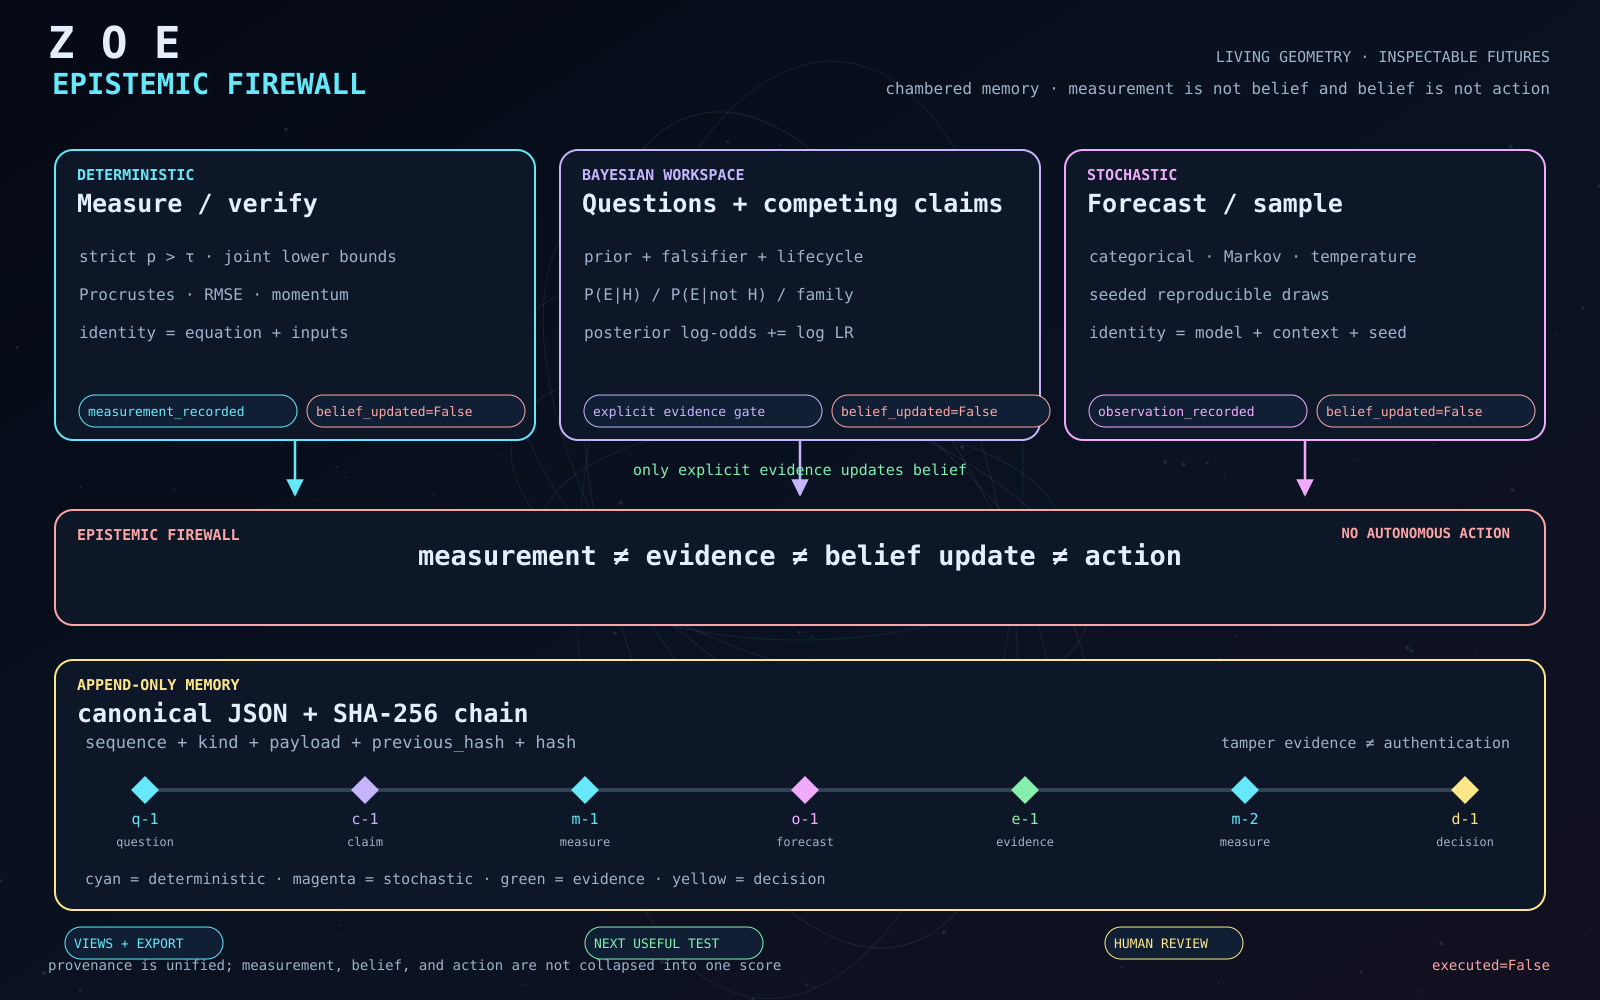
\includegraphics[width=\textwidth]{epistemic-firewall.png}
\caption{The Zoe epistemic firewall. The later self-governing extension changes execution authority only inside a separately declared in-memory loop; it does not erase these epistemic distinctions.}
\label{fig:firewall}
\end{figure}

The native components have distinct scopes:
\begin{itemize}
  \item \textbf{HELEN} supplies lazy scenes, direct interaction, accessible-volume controls, and compressed held-out categorical predictions.
  \item \textbf{Ablation + GEM} supplies native GTK hosting, Spatial IR, Lab sessions, VDI replay, source constraints, and evidence export.
  \item \textbf{Cerotto GEM} supplies read-only forensic cases, guarded evidence actions, vault timelines, and a separate C11 engine and permission model. Zoe does not absorb its database or authority.
  \item \textbf{BRAIN and the field notebook} supply observation state, deterministic recommendations, Bayesian claims and evidence, deterministic/stochastic chambers, and next-test ranking.
  \item \textbf{Cognitive Field and Presence} supply bounded symbolic proposals, state reflection, and an explicitly bounded self-model.
  \item \textbf{PALA} is an optional recovery companion for signature carving and filesystem recovery. Recovered content is not thereby authentic, complete, or safe.
\end{itemize}

\section{Bayesian field notebook}
Questions contain independent binary claims with priors, current posteriors, falsifiers, and lifecycle states. Claims are not forced into a mutually exclusive set. For prior $p$ and supplied likelihoods $L_T=P(E\mid H)$ and $L_F=P(E\mid\neg H)$, an explicit evidence event updates
\begin{equation}
\operatorname{logit}(p')=\operatorname{logit}(p)+\log\frac{L_T}{L_F},
\qquad
\operatorname{logit}(p)=\log\frac{p}{1-p}.
\label{eq:bayes-logit}
\end{equation}
Equivalently, the likelihood ratio is added in log-odds space. Every update preserves the evidence source, likelihood ratio, log likelihood ratio, prior and posterior log-odds, previous and new posterior, and belief diff. Negative and mixed evidence remain in the history.

Posteriors are conditional on the supplied likelihood model, not objective truth scores. Evidence families prevent derivative or correlated sources from silently becoming independent confirmation. Repeating a family requires explicit dependence acknowledgment and adjusted likelihoods. This is a software guard for disciplined bookkeeping, not an automatic estimator of the correct dependence model.

Next-test prioritization uses the declared heuristic
\begin{equation}
\operatorname{priority}(q)=\frac{v_q\,g_q}{\varepsilon_q},
\label{eq:priority}
\end{equation}
where $v_q$ is decision value, $g_q$ expected information gain, and $\varepsilon_q>0$ estimated effort. In the original notebook this ranks attention only: it is not a probability, learned reward, discovered utility, or authorization rule. The later autonomy loop reuses the same arithmetic as an internal proposal utility, a change in control semantics that must be stated rather than hidden.

\begin{figure}[htbp]
\centering
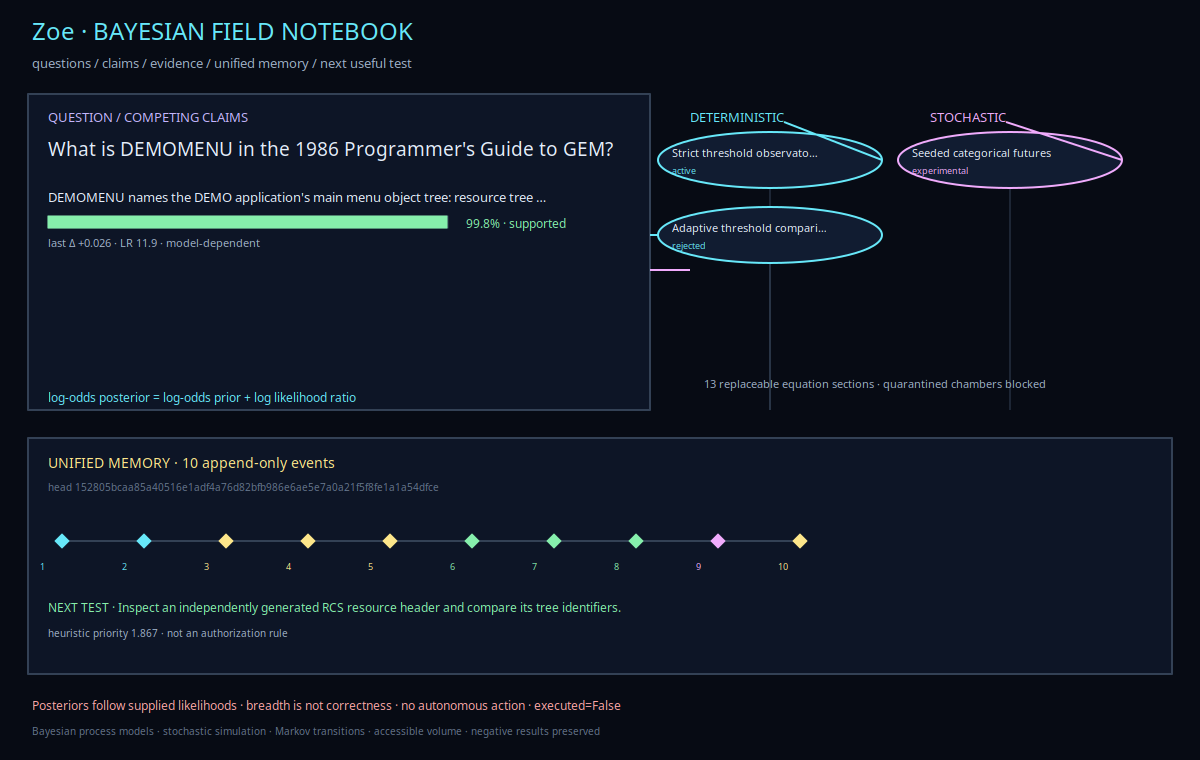
\includegraphics[width=\textwidth]{field-notebook.png}
\caption{Zoe's Bayesian field notebook: explicit evidence updates, deterministic and stochastic chambers, append-only memory, and review-required next-test recommendations.}
\label{fig:notebook}
\end{figure}

The worked DEMOMENU example investigates a definition in the 1986 \emph{Programmer's Guide to GEM}. It retains a primary-source definition, version-dependent counterevidence, initialization-code observations, a strict measurement, a seeded stochastic chamber, and a next-test recommendation. Its value is the inspectable belief history rather than the posterior percentage alone.

\section{Chambers and replayable memory}
The equation registry contains 13 replaceable sections: binary Bayesian updates, strict volume, forecast measurement, adaptive volume, joint volume, momentum, temperature, categorical sampling, Markov steps, bounded continuations, timing RMSE, Procrustes alignment, and inspection priority. Custom functions are registered through a Python API without \texttt{eval}. Deterministic chambers record reproducible measurements; stochastic chambers record forecasts, transitions, transforms, and seeded samples. Quarantined chambers remain inspectable but cannot run.

For sequence $s_i$, event kind $k_i$, payload $p_i$, and previous hash $h_{i-1}$, the canonical chain is
\begin{equation}
h_i=\sha\!\left(\canonical(s_i,k_i,p_i,h_{i-1})\right).
\label{eq:memory-chain}
\end{equation}
Loading recomputes the complete chain and rejects edited or reordered events. Probability vectors of at most 64 values are stored completely; longer vectors are represented by length and SHA-256 digest to bound memory. No-overwrite saves protect earlier exports.

\begin{figure}[htbp]
\centering
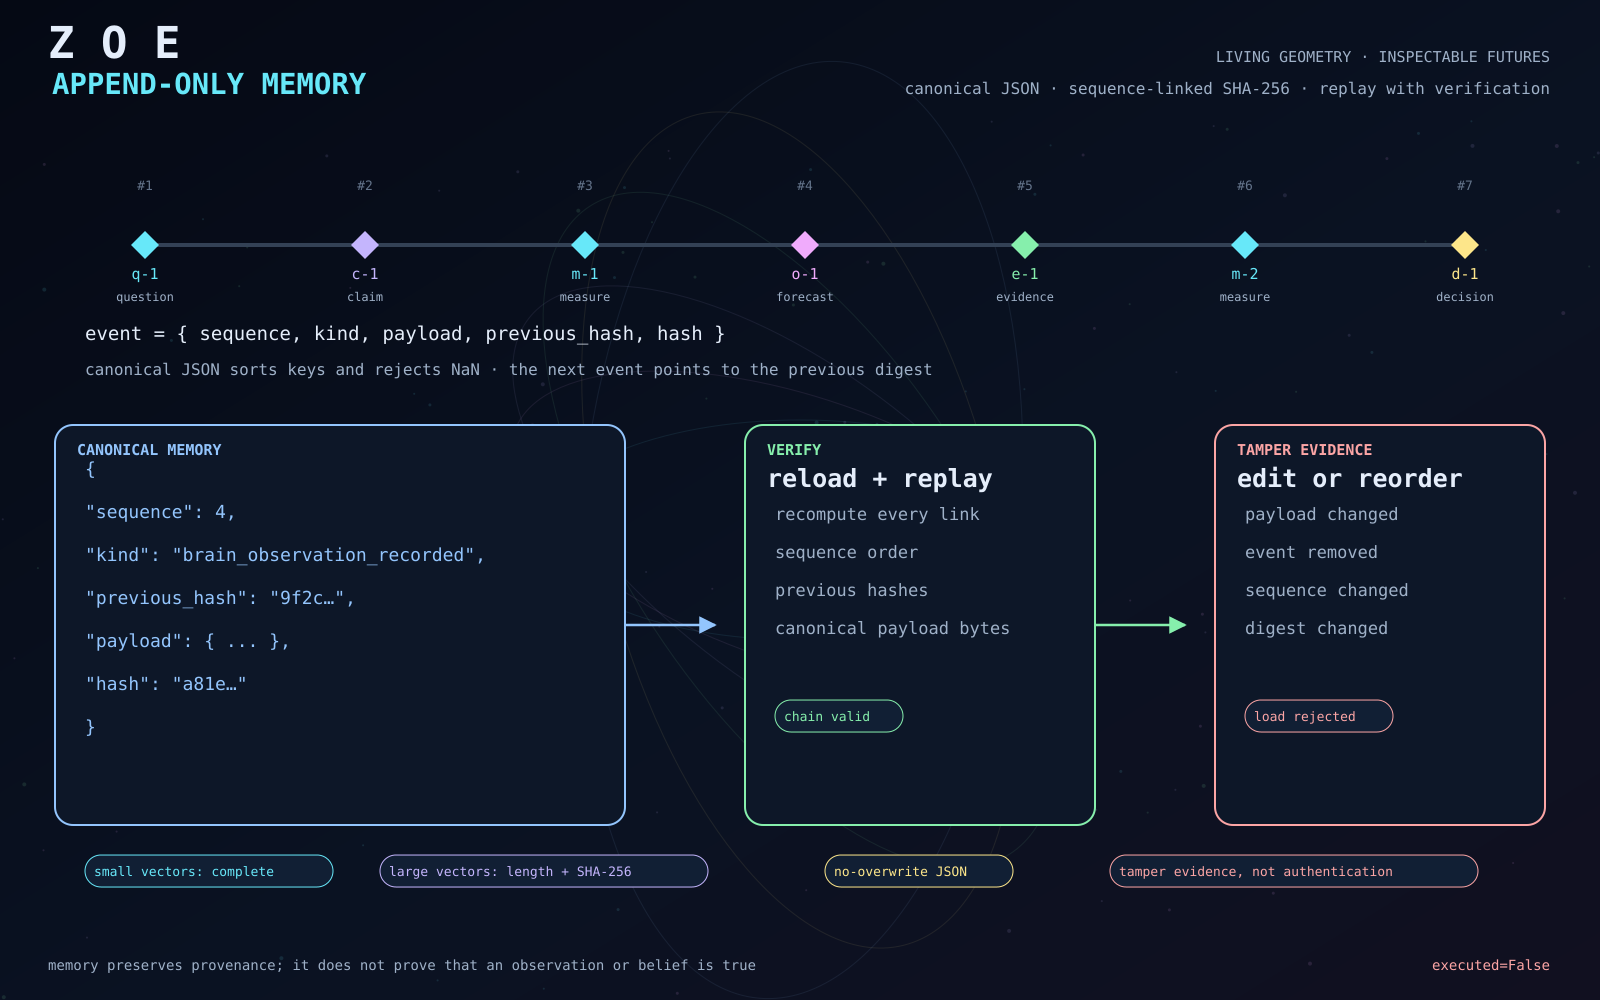
\includegraphics[width=\textwidth]{memory-chain.png}
\caption{Append-only Zoe memory records distinct event kinds and makes alteration visible. Hash chaining supplies tamper evidence, not authentication or proof that a recorded claim is true.}
\label{fig:memory}
\end{figure}

The integrated knowledge graph applies the same canonical-event discipline to repository observations and declared links. A source observation records repository, revision, and scope; a declared link does not transfer evidence or permission. Source presence is not runtime verification. These distinctions are central when multiple independently governed components appear in one interface.

\section{Cog: a bounded categorical token processor}
Zoe Cog is a deliberately small trainable bigram processor, not an LLM. For context token $u$, let $n_u(a)$ be the observed count of candidate $a$, $N_u=\sum_an_u(a)$, and $q(a)$ the unigram prior. With smoothing $\alpha\in(0,10]$,
\begin{equation}
\widetilde p(a\mid u)=\frac{n_u(a)+\alpha q(a)}{N_u+\alpha},
\qquad
p(a\mid u)=\frac{\widetilde p(a\mid u)}{\sum_{b\in\mathcal O}\widetilde p(b\mid u)}.
\label{eq:cog-bigram}
\end{equation}
Backward walks apply the same construction to reversed transition counts and reverse unigram counts. Each walk selects maximum probability with lexical tie-breaking and measures the complete distribution using the unchanged strict operator. Reversing a transition relation does not reverse meaning, causality, or time.

Cog exposes forward and backward walks, complete probabilities, source hashes, volume bands, and experimental temperature steering. Generated walks are review-required and do not assert facts or authorize commands. The small vocabulary makes the processor suitable for deterministic counterfactual experiments in the autonomy study, but token interventions are not distributions over feasible real-world actions.

\section{Cognitive Field, BRAIN, and Presence}
\subsection{Bounded symbolic proposal generation}
The Cognitive Field implements a bounded General Symbol Processor, where ``general'' refers to explicit text, tags, record IDs, revisions, and human-readable rule descriptions rather than unrestricted intelligence. Sourced inputs enter a bounded FIFO working set. Declarative storage and retrieval check revisions. A procedural rule $r$ with required tag set $T_r$ matches working-set tags $T_W$ when
\begin{equation}
\operatorname{Match}(r,W)=\indicator[T_r\subseteq T_W].
\label{eq:cognitive-match}
\end{equation}
Rules contain no executable code. A successful match can prepare a proposal, but in the original Zoe build it remains \texttt{review\_required=True}, \texttt{belief\_updated=False}, and \texttt{executed=False}. The worked example uses capacity four, records an eviction, preserves a revision mismatch, and shows that only one of two declared rules matches. This is symbolic software behavior, not a validated model of biological memory, ACT-R, Spaun, or consciousness.

\begin{figure}[htbp]
\centering
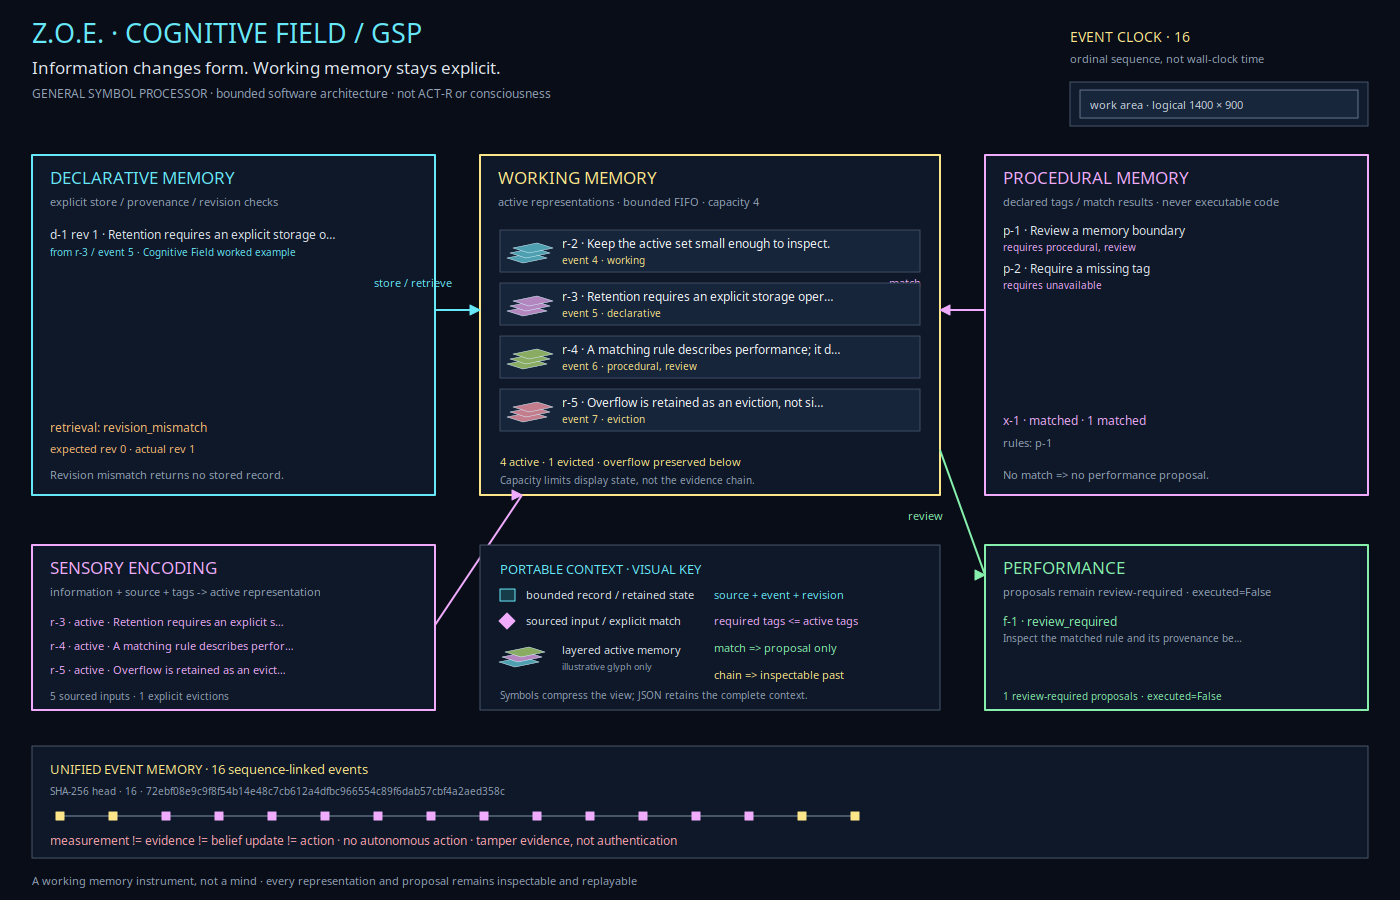
\includegraphics[width=\textwidth]{cognitive-field.png}
\caption{Zoe's Cognitive Field: sourced bounded working memory, declarative revision checks, procedural matching, and review-required proposals.}
\label{fig:cognitive}
\end{figure}

\subsection{Deterministic observation and recommendation}
BRAIN records forecast and evidence state and returns a deterministic module/action recommendation. In schematic form,
\begin{equation}
o_t=M_{\mathrm{BRAIN}}(S_t,C_t),\qquad
r_t=R_{\mathrm{BRAIN}}(o_t),
\label{eq:brain}
\end{equation}
where $r_t$ is advice, not execution. The autonomy benchmark exercises four states: an in-band correct forecast, a broad out-of-band forecast, an incorrect forecast, and an in-band correct forecast after evidence export. They yield four distinct recommendations: \texttt{research/preserve}, \texttt{volume/inspect}, \texttt{research/inspect}, and \texttt{horizon/inspect}. This variation supplies the state-responsiveness dimension later denoted $R$.

\subsection{Self-model boundary}
Presence preserves reflections, uncertainty, provenance, and a self-model while explicitly recording that a self-model is not a self. Self-reports can be evidence about the system's generated representation; they are not self-certification of experience, correctness, or autonomy. Presence does not turn a high accessible-volume count or a proposal into phenomenal perception.

\begin{figure}[htbp]
\centering
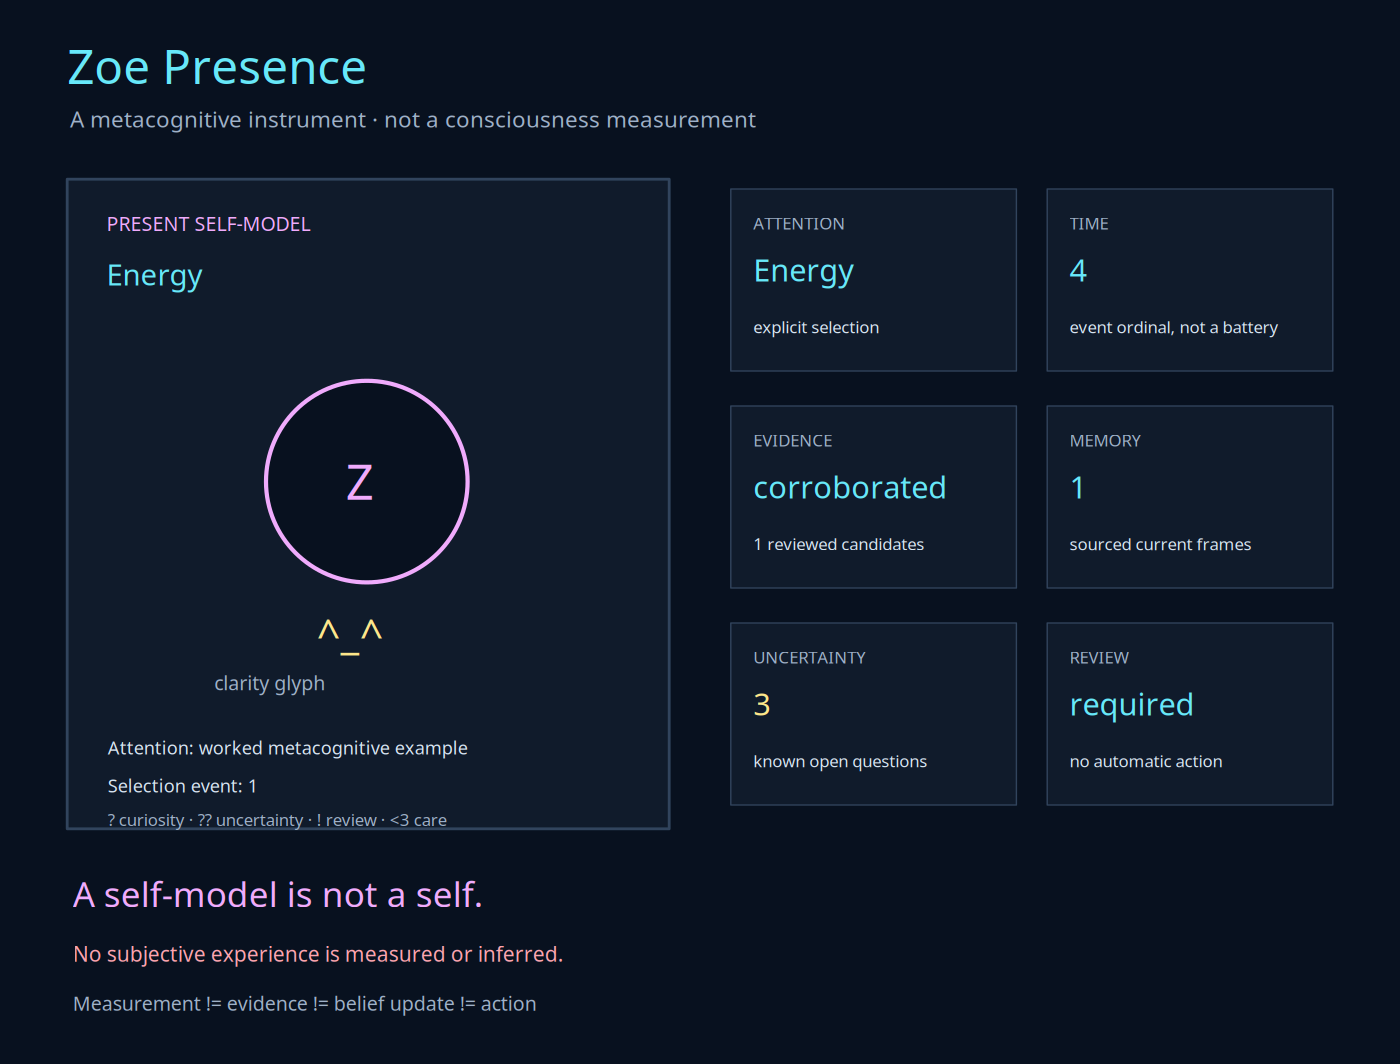
\includegraphics[width=\textwidth]{presence.png}
\caption{Presence exposes a bounded self-model and review boundary without treating self-description as proof of a self.}
\label{fig:presence}
\end{figure}

\section{Native geometry and evidence export}
The native Geometry Atlas supplies similarity, rigid, and affine Procrustes alignment, ellipse families, parabolic envelopes, modular clocks, hub-and-loop graph invariants, accessible-volume controls, and an Onset Lab. Spatial IR scenes can be exported to SVG, PNG, and real little-endian GEM VDI. Headless export does not require GTK. Source-constraint and VDI-roundtrip checks concern deterministic geometry and file behavior, not whole-shape, anatomical, or semantic correctness.

The integrated environment also connects ten source repositories through twelve launch or inspection endpoints in the historical allgems distribution. Each component retains its dependencies, evidence stores, and guards. A plan label cannot prove physical behavior, and a unified interface is not a universal enforcement mechanism.

\section{CERN evidence and virtual workbenches}
\subsection{Inventory, provenance, and process ownership}
The CERN Workbench connects the read-only CERN and Digital Research evidence collections to Zoe-owned process lifecycle controls, HELIOS, and Atelier \cite{zoecernworkbench}. Its handover records 9,968 CERN inventory entries and 226 document previews. The Evidence Navigator's schema-v2 index divides those previews into C1 foundational (40), C2 subsystem (49), C3 integrated (125), and C4 cross-domain (12). Full verification checks 226 source hashes, 226 preview hashes, 226 compatibility links, and 17 bridge-document links. A preview is navigation evidence, not a complete explanation or live detector state \cite{zoevidenceguide}.

The console bridge attaches to a healthy existing loopback server or starts a new one on a free port. It records process ownership and stops only a process it started whose command still matches the expected checkout; it does not terminate an attached user-owned server. Browser opening, XTEST input, and serial emission require explicit actions. Corpus inspection starts no process and accesses no physical hardware.

\begin{figure}[htbp]
\centering
\begin{tabular}{@{}c@{}c@{}}
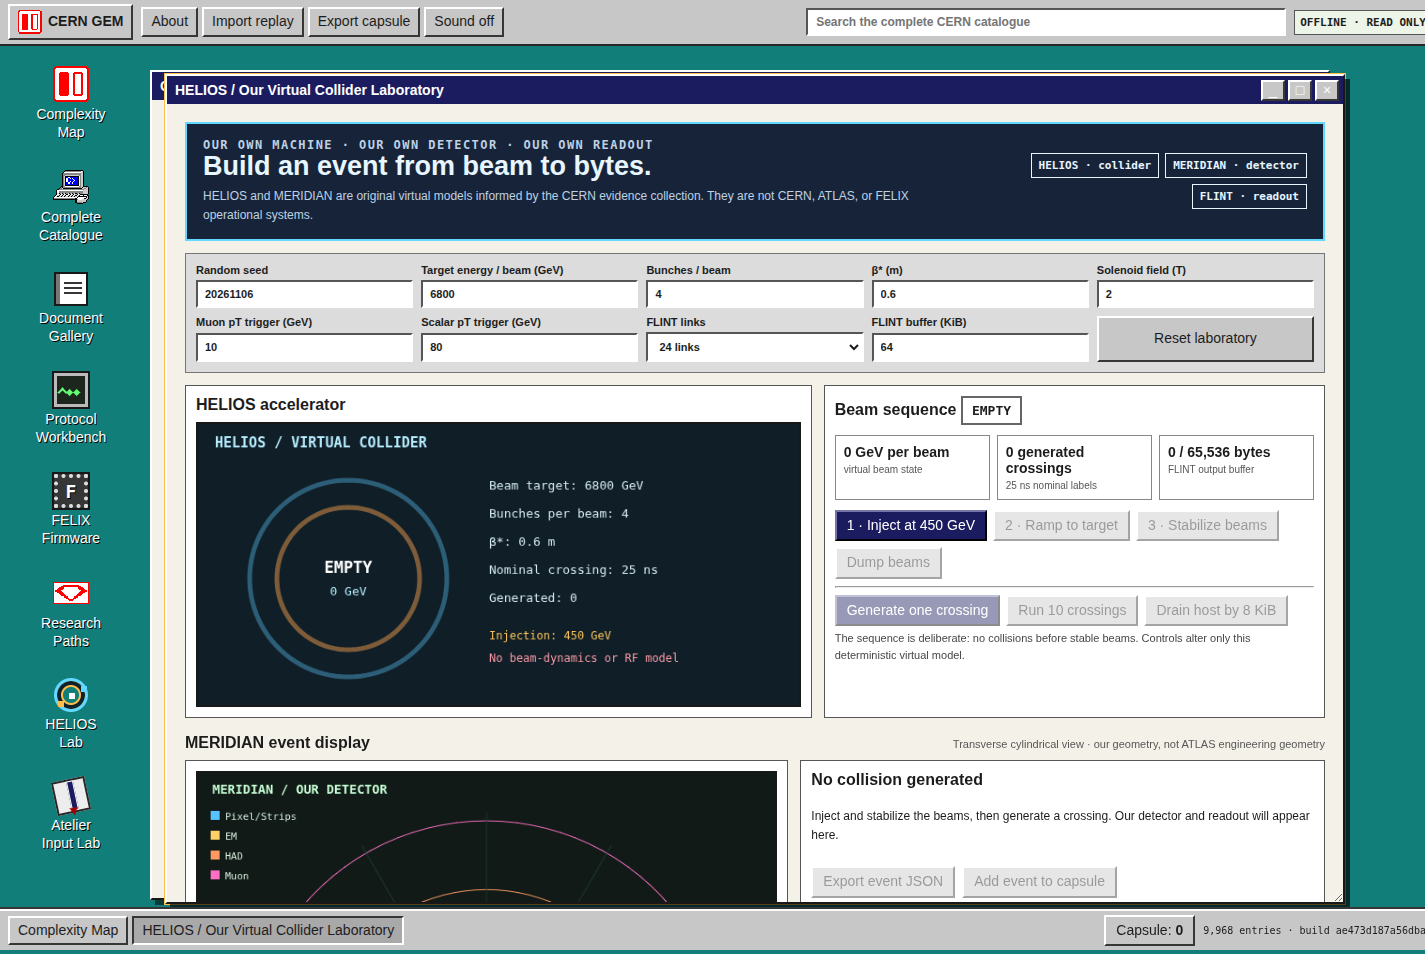
\includegraphics[width=0.48\textwidth]{zoe-helios.png}&
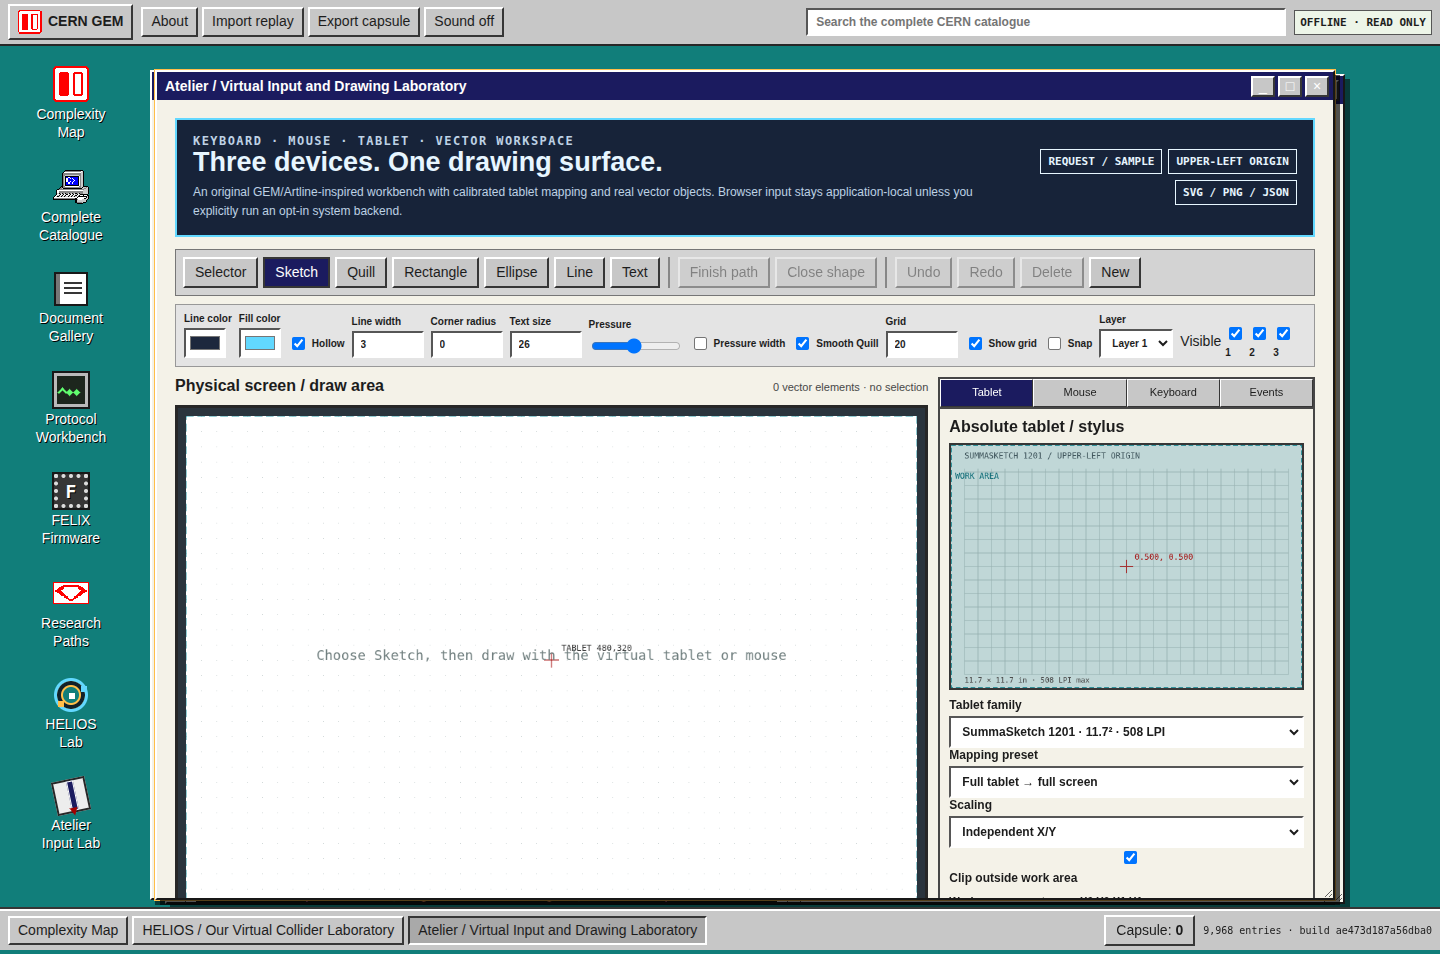
\includegraphics[width=0.48\textwidth]{zoe-atelier.png}
\end{tabular}
\caption{HELIOS and Atelier are virtual collider, input, drawing, and replay laboratories. Their scenes and input models do not imply a physical accelerator connection.}
\label{fig:cern-virtual-labs}
\end{figure}

The historical handover recorded 39/39 Zoe stress tests, 20/20 GEM stress tests, 5/5 CERN corpus tests, 75 Python tests, three JavaScript model suites, and 130 browser checks passing, including isolated live tests only when explicitly enabled. These are scoped implementation checks, not hardware validation.

\subsection{Seven evidence bridges and synthetic timing}
The Evidence Navigator implements seven bridges: timing-aware readout replay, a protocol observation ladder, guarded observability, scene/audio sonification, deterministic shadow retrieval, cross-experiment design review, and C1--C4 practice. Its default timing replay uses 24 channels, 64 events, a 40.08 MHz reference, an eight-slot buffer, 256-byte descriptors, and host consumption every third event. CRC32 protects descriptor integrity but is not a signature. Outputs retain \texttt{hardware\_accessed=false}, \texttt{measured=false}, and \texttt{physical\_connection\_claimed=false}.

The same replay can generate deterministic 16-bit mono PCM audio. Sonification is another view of the recorded synthetic state, not detector sound, an alarm, or a health signal. A shadow query returns saved finding fields without an LLM; a negative static timing result is not automatically a deployed runtime failure.

\subsection{Protocol Lab: recovered framing without device commands}
The Protocol Lab independently implements documented SPECS and AMAC examples \cite{zoeprotocolguide}. The SPECS first header byte is
\begin{equation}
H_0=(\operatorname{slave\ address}\ll2)\,|\,\operatorname{mode}.
\end{equation}
For header bytes $H_0,H_1,H_2$ and check byte $H_3$, the demonstrated nibble check is
\begin{equation}
C=\left(\bigoplus_{i=0}^{2}((H_i\gg4)\oplus(H_i\,\&\,0x0F))\right)\oplus(H_3\gg4),
\qquad H_3\,\&\,0x0F=C.
\end{equation}
Payload bytes are XOR-checked and sent least-significant-bit first; a ninth marker bit identifies the final payload byte. These checks provide integrity information, not authentication.

The recovered short/long boundary is
\begin{equation}
\operatorname{long}=\indicator[\operatorname{read\ count}>0x80],
\qquad \operatorname{reported\ count}=\operatorname{read\ count}\,\&\,0x7F.
\end{equation}
Thus 128 is not long and reports zero, while 129 is long and reports one. Focused RTL evidence covers all 256 counts and 1,280 checks. AMAC read-next independently increments a three-bit sequence and eight-bit address with wraparound; returned data values are supplied separately. The laboratory regenerates models and recorded examples without issuing device commands.

\begin{figure}[htbp]
\centering
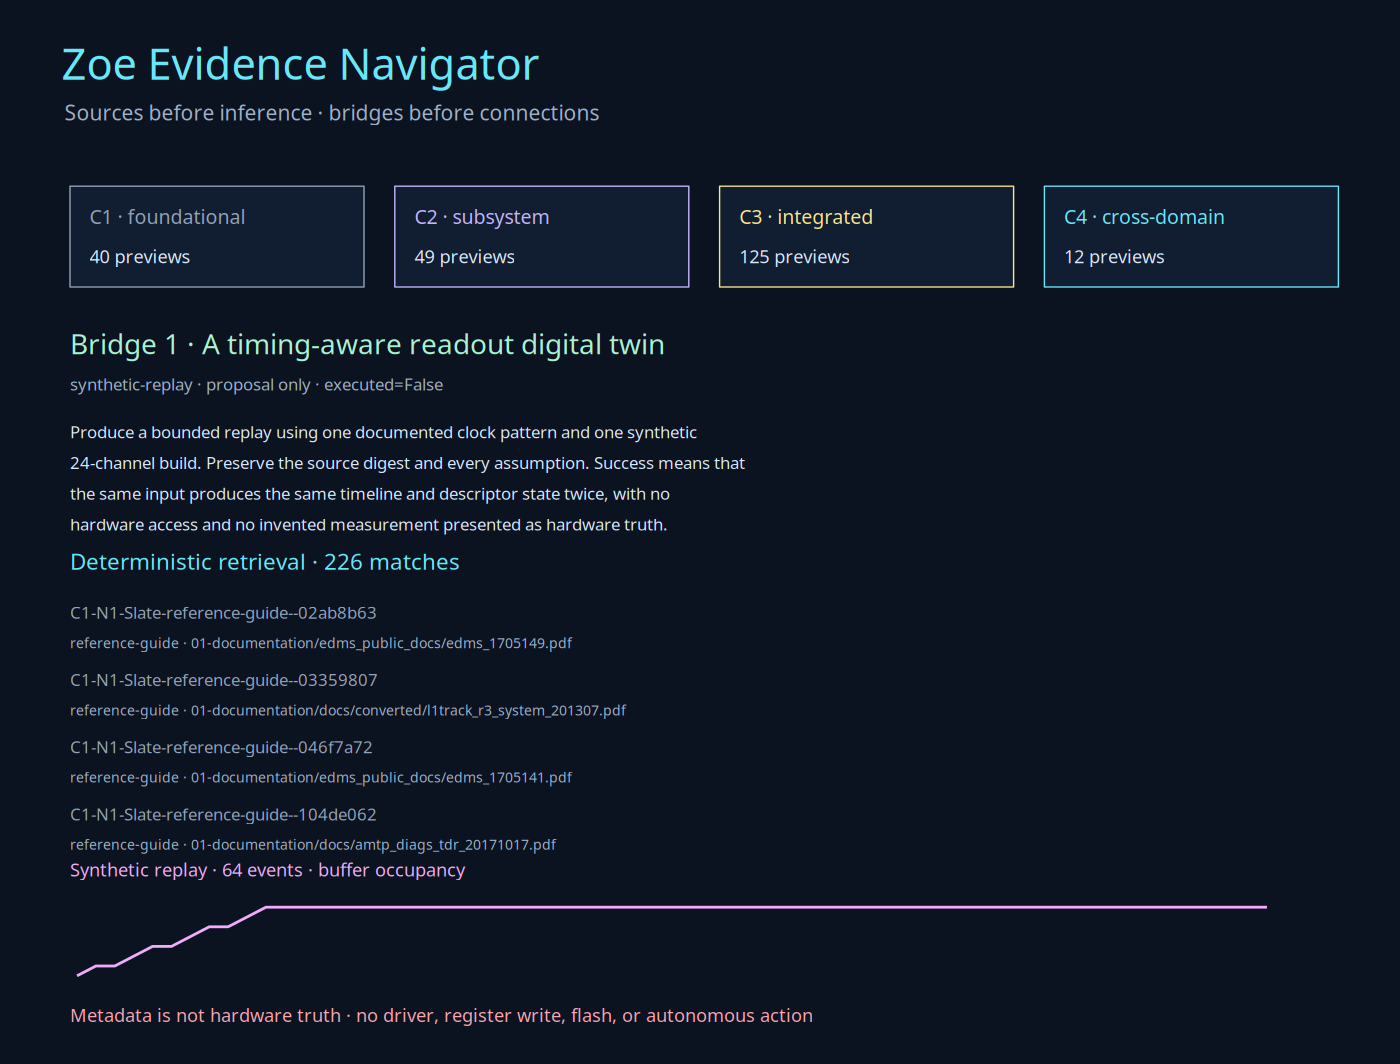
\includegraphics[width=\textwidth]{zoe-evidence.png}
\caption{Zoe Evidence Navigator: cited retrieval, source verification, bounded replay, and guarded observation. Source previews do not become live detector health.}
\label{fig:zoe-evidence-navigator}
\end{figure}

\subsection{Waveform replay and corroboration limits}
Waveform Replay reads bounded VCD, JSONL, and optional legacy WDB windows while preserving declarations, retained events, timestamps, truncation, source hashes, and normalized-document digests \cite{zoewaveformguide}. Replay is not acquisition. For clock corroboration, the classifier examines the initial payload and the first 32 subsequent equal intervals and alternating transitions. A complete sampled signature may be corroborated, ambiguous when candidates share a period or initial state, or unmapped. Matching a period alone is insufficient, and even a unique sampled period does not prove identity outside the retained window.

The cited external CERN mapper processed 10,759,544 events across 363 storage streams and reported one corroborated clock, two ambiguous streams, and 360 unmapped streams. Zoe does not rerun that large analysis or bundle its raw waveform corpus. Its independently tested preview uses four synthetic traces and preserves duplicate-signature ambiguity.

\begin{figure}[htbp]
\centering
\begin{tabular}{@{}c@{}c@{}}
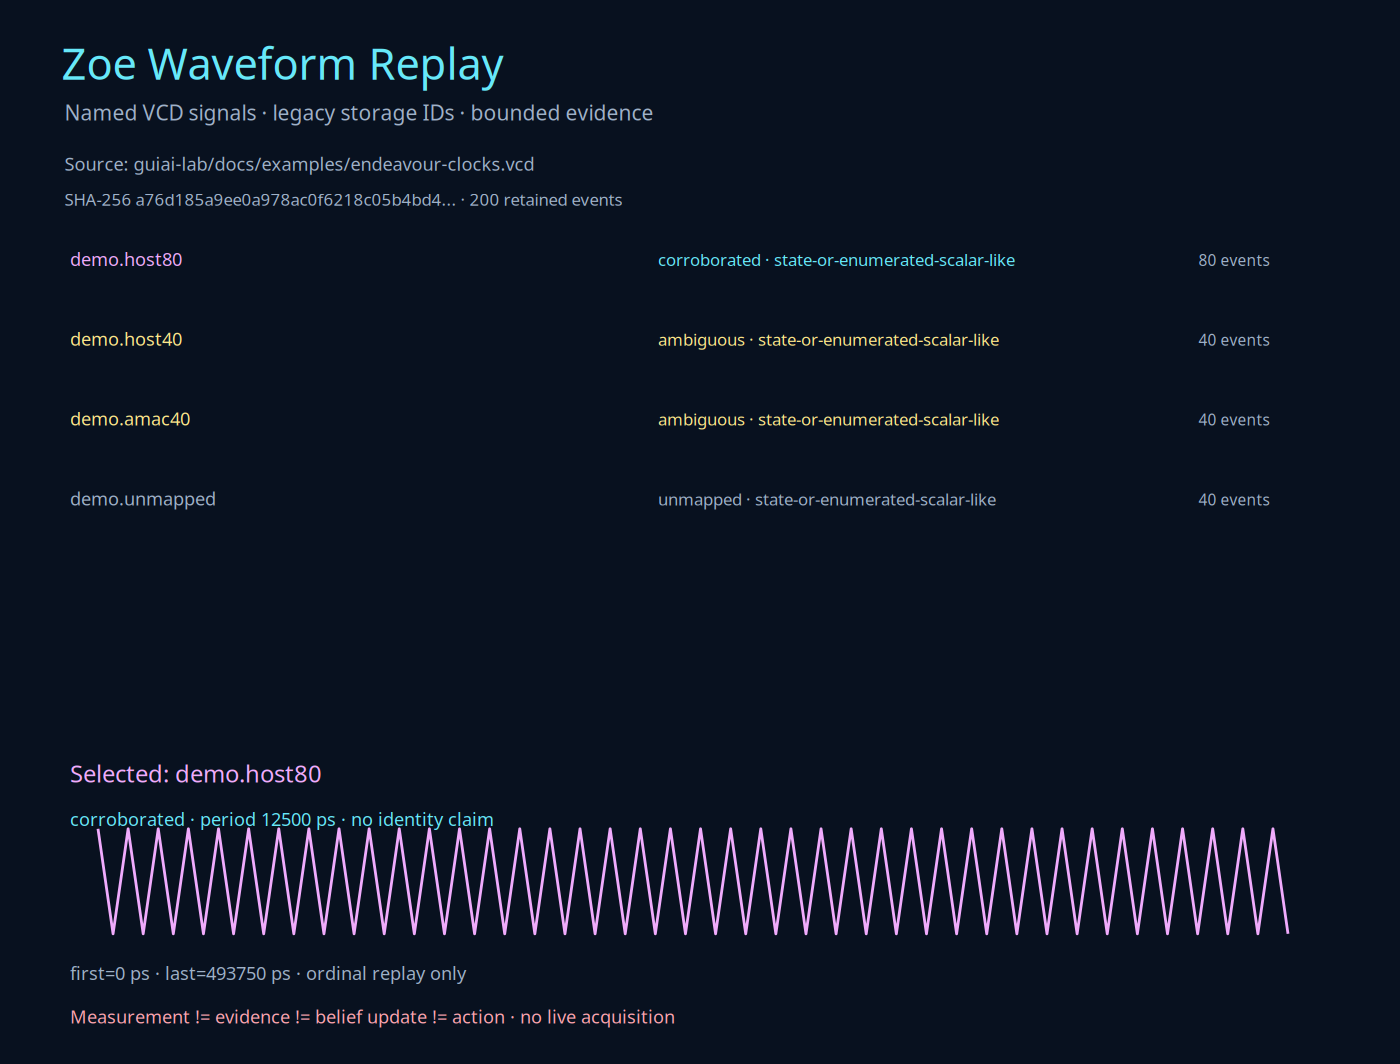
\includegraphics[width=0.48\textwidth]{zoe-waveform.png}&
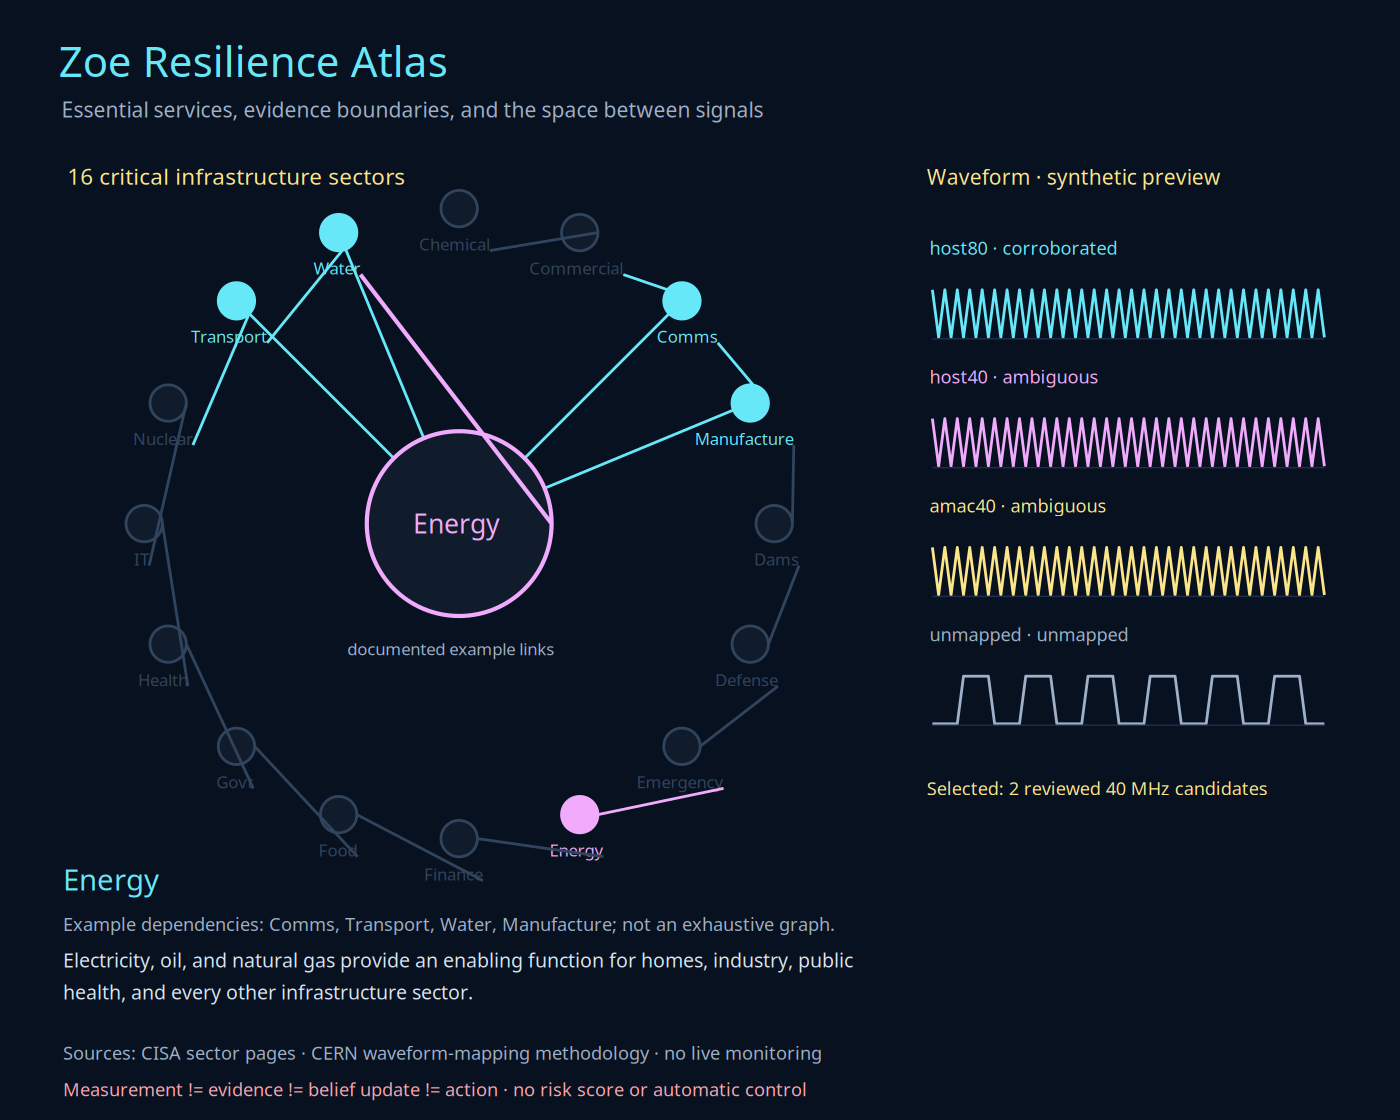
\includegraphics[width=0.48\textwidth]{zoe-resilience.png}
\end{tabular}
\caption{Waveform Replay and the Resilience Atlas preserve evidence limits. Neither performs live acquisition, infrastructure monitoring, risk scoring, or hardware control.}
\label{fig:waveform-resilience}
\end{figure}

The Resilience Atlas combines original summaries of the 16 US critical-infrastructure sectors with this small signature laboratory. Dependency links are selected public examples, not causal or exhaustive models. It contacts neither CISA nor CERN and assigns no sector risk score.

FELIX observations describe source artifacts rather than connected hardware or live detector health. The Protocol Lab preserves recovered SPECS serial-framing and AMAC reply examples with checksum and long-read boundaries; its displayed records are model and recorded examples, not new proof of correctness or permission to issue device commands.

\begin{figure}[htbp]
\centering
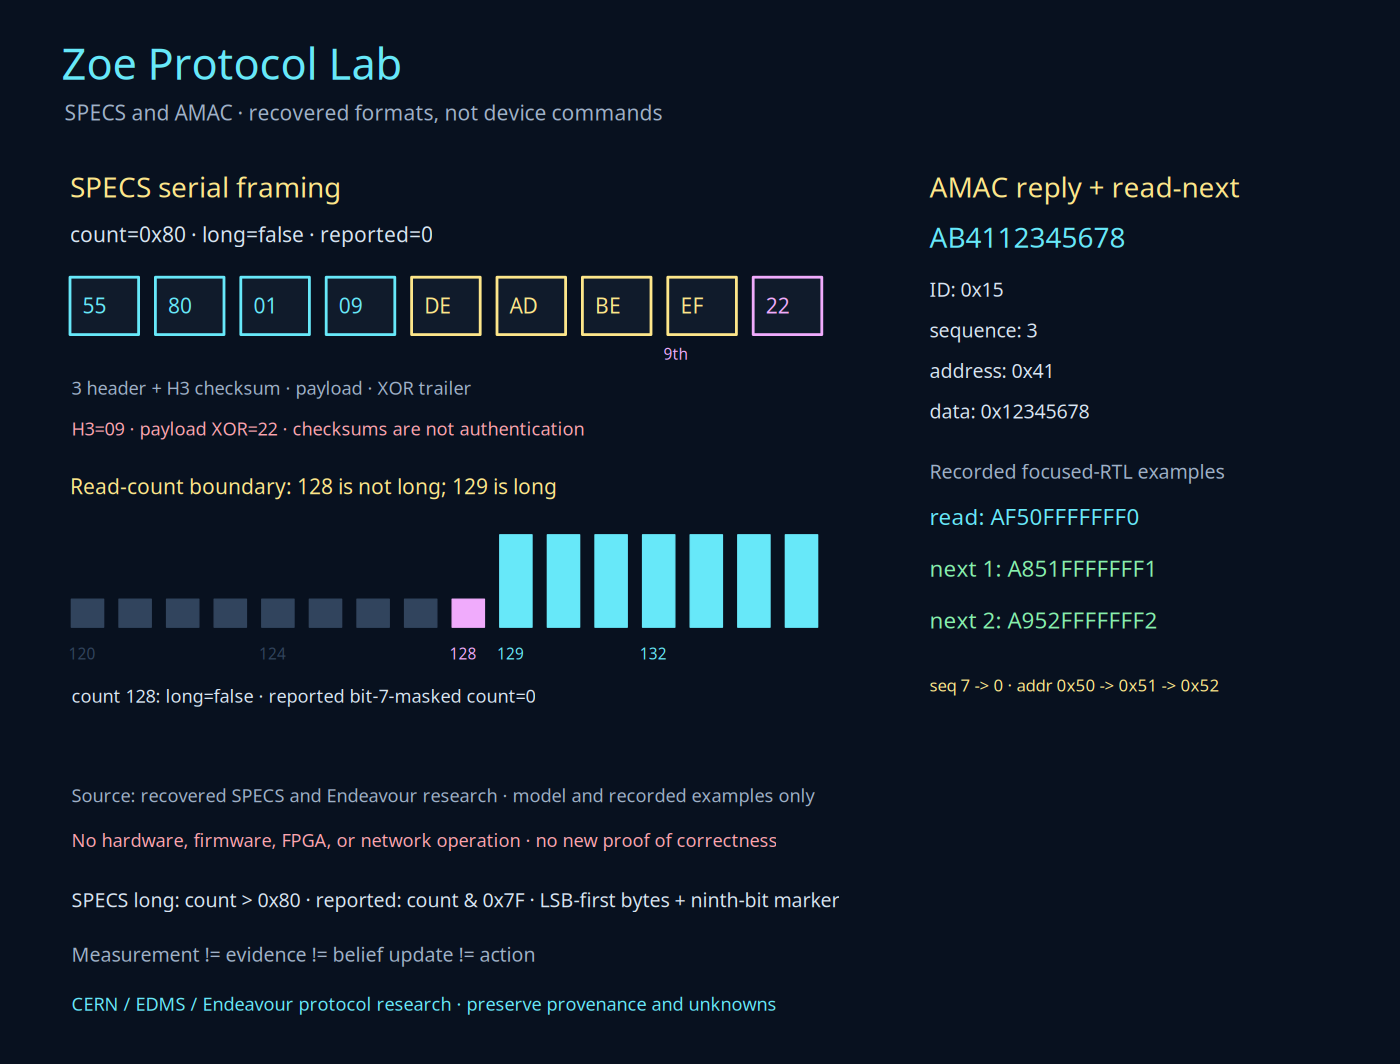
\includegraphics[width=\textwidth]{protocol.png}
\caption{Zoe Protocol Lab: recovered SPECS and AMAC protocol examples. No hardware, firmware, FPGA, or network operation is performed, and checksums are not authentication.}
\label{fig:protocol-lab}
\end{figure}

Patchbay separately inspects firmware formats and signs new update capsules. Its acceptance condition requires
\begin{equation}
\text{authenticity established}=
\text{signature valid}\;\land\;\text{artifact match}\;\land\;\text{trusted-key match}.
\label{eq:patchbay-authenticity}
\end{equation}
A self-contained public key alone is not publisher trust. Acceptance commands require an explicit execution flag and declared writes require a separate hardware-write flag. No physical hardware operation was executed for the paper integration.

\begin{figure}[htbp]
\centering
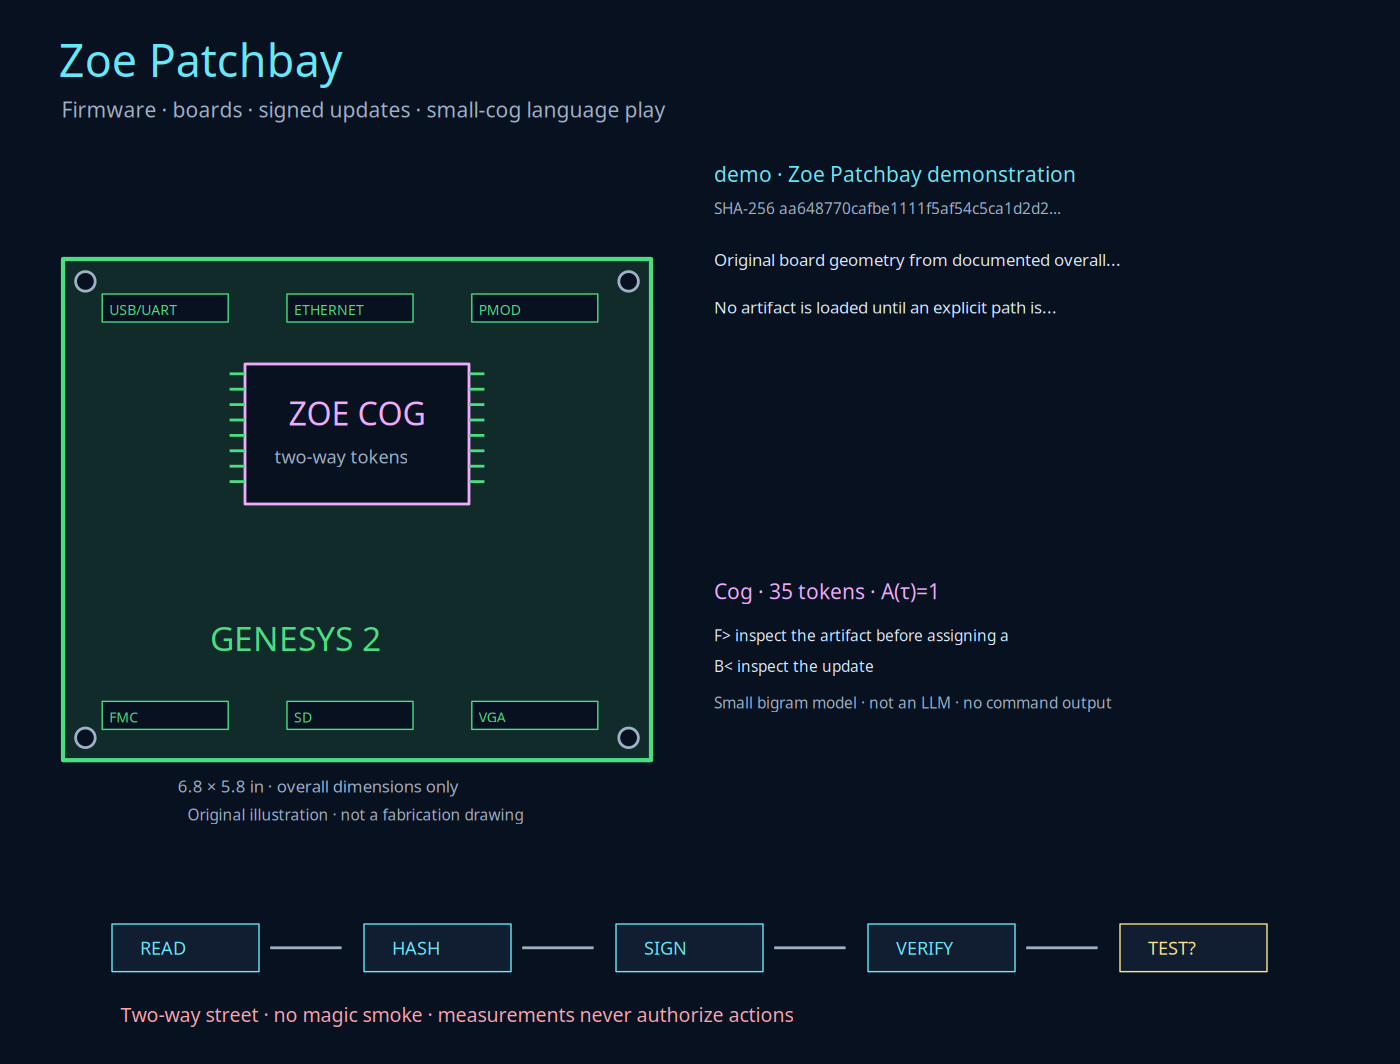
\includegraphics[width=\textwidth]{patchbay.png}
\caption{Zoe Patchbay: firmware inspection, hashing, signing, verification, and explicit acceptance boundaries. The board illustration is not a fabrication drawing and Cog output is not a command channel.}
\label{fig:patchbay}
\end{figure}

\section{Scoped verification and later audit}
The original Zoe proof of concept recorded the matrix in Table~\ref{tab:zoe-verification}. These are historical, component-scoped software results, not independent scientific replication.
\begin{table}[htbp]
\centering
\caption{Verification matrix preserved from the original Zoe proof of concept.}
\label{tab:zoe-verification}
{\scriptsize
\begin{tabularx}{\textwidth}{p{3.7cm}p{3.3cm}X}
\toprule
Area&Recorded result&Scope\\
\midrule
Zoe native&25 passed&X11 observation, notebook, host launch, Allen atlas, research, and export workflows\\
Zoe headless&21 passed, 4 native-only skips&Core, Allen atlas, memory, CLI, and evidence behavior without display\\
brain-gem headless&13 passed, 3 native-only skips&Standalone notebook, chambers, memory, and CLI\\
Broader GEM native&20 passed&Constraints, VDI, replay, dragging, and exports\\
Accessible Q-Volume&Toy arithmetic passed&Strict equality, filtrations, $-1$/$+3$ changes, and two-way JSON\\
Research conformance&17 passed&Strict volume, Procrustes, toy continuations, rhythm evidence, and Bayesian updates\\
Original model cases&16 verified&Saved distributions, ranks, counts, entropy, and hashes\\
BioBERT&120 cases, 54 candidates&Independent metrics and split recomputation\\
Cerotto&64 normal and 64 sanitizer passed&One EWF-dependent skip per suite\\
PALA&25 Rust tests, 125 integration checks&Two optional skips; recovery and format behavior\\
Interactive browser&23 particles, zero external requests/errors&Desktop, mobile, reduced motion, and controls\\
Packaging&Wheel and source distributions passed&Installed notebook, HELEN asset, conformance, and export checks\\
\bottomrule
\end{tabularx}}
\end{table}

A later November 7 audit of Zoe revision \texttt{8fcdcfe4} directly exercised both accessible-volume implementations, verified the strict comparison and threshold equality exclusion, rehashed and reloaded the 23-event knowledge chain, and recomputed all sixteen comparison and 120 BioBERT cases without fresh inference. A focused integration run completed 24 tests: 23 passed and one native-only test skipped. An isolated native unified test then failed because \texttt{UnifiedNativeCase} still expected eleven links after recording a Kevlar source while the implementation intentionally recorded both the observation and its declared Zoe link, producing twelve. The stale assertion remained an open engineering follow-up in that audit.

The audit also noted the absence of a root integrated CI workflow, a comparison verifier that rewrites tracked summaries and timestamps, two documentation inconsistencies, and the lack of a tagged PDF structure tree. Earlier all-pass records are not substituted for these later observations. The audit was not an exhaustive security review, fresh model benchmark, hardware validation, or certification of deployed behavior. This monograph preserves both the positive checks and the unresolved engineering findings.

\section{From review-gated Zoe to an executable internal loop}
The original proof of concept explicitly disclaimed autonomous decision-making. Its measured agency stopped at proposals and recommendations. The next part describes a separate extension that adds goal authorship, value-based selection, and guarded in-memory execution. The extension does not retrospectively change the evidence status of every Zoe component: most modules remain review-gated, external actuation remains prohibited, and the full-autonomy predicate applies only to the newly implemented loop.

\clearpage
\part{The Self-Governing Measurement--Action Loop}

\section{From observation to effective perception}
The master protocol begins with computational state $S_t$, supplied context $C_t$, and an instrument $M$:
\begin{equation}
O_t=M(S_t,C_t).
\label{eq:observation}
\end{equation}
An observation is not a complete description of state. For policy $\pi(a\mid c)$ and explicit intervention $\doop(z)$, define the policy effect in bits:
\begin{equation}
D_z=\KL\!\left(\pi(a\mid\doop(z),c)\,\middle\|\,\pi(a\mid c)\right)
=\sum_a\pi_z(a)\log_2\frac{\pi_z(a)}{\pi(a)}.
\label{eq:policy-effect}
\end{equation}
Effective perception counts alternatives that are both accessible and causally effective on the declared policy:
\begin{equation}
P_{\tau,\delta}=\sum_{z\in Z}\indicator[p(z)>\tau]\,\indicator[D_z>\delta].
\label{eq:effective-perception}
\end{equation}
Per-context coverage and suite summaries are
\begin{align}
E_{\tau,\delta}&=
\begin{cases}
P_{\tau,\delta}/A_\tau,&A_\tau>0,\\
\text{undefined},&A_\tau=0,
\end{cases}\\
E_{\mathrm{micro}}&=\frac{\sum_iP_{\tau,\delta,i}}{\sum_iA_{\tau,i}},
\qquad
E_{\mathrm{macro}}=\frac{1}{|\{i:A_{\tau,i}>0\}|}
\sum_{i:A_{\tau,i}>0}E_{\tau,\delta,i}.
\end{align}
If $\pi_z(a)>0$ where $\pi(a)=0$, the divergence is infinite. The implementation preserves that support mismatch explicitly and counts the intervention as effective rather than hiding it with an arbitrary smoothing constant.

Effective perception is an operational construct, not phenomenal experience. A large $D_z$ can occur in an externally manipulated system; causal sensitivity is not action authorship. It supplies a more policy-relevant measurement than raw breadth while leaving goal and intervention origin to later stages.

\section{Declared value and the master composition}
For prior belief $b$, posterior $b_z$, declared utility $U$, and optimal actions $a_0^*$ and $a_z^*$ before and after observation $z$, perceived-information value is
\begin{equation}
V(z,c)=\mathbb E_{x\sim b_z}[U(a_z^*,x,c)]
-\mathbb E_{x\sim b}[U(a_0^*,x,c)].
\label{eq:information-value}
\end{equation}
This quantity is relative to the declared belief and utility models. It does not establish intrinsic preferences or that the system cares.

The master measurement--action composition is
\begin{equation}
\boxed{
\begin{aligned}
(S_{t+1},R_{t+1})={}&
\operatorname{Execute}_{\alpha_t}
\circ\operatorname{Guard}_{G,\Pi}
\circ\operatorname{Value}_{U}\\
&\circ\operatorname{Propose}_{\pi}
\circ\operatorname{Perceive}_{\tau,\delta}
\circ M(S_t,C_t).
\end{aligned}}
\label{eq:master}
\end{equation}
Read right to left, the stages are observation, effective perception, proposal generation, valuation, goal-and-policy guarding, and execution or no-op. The early evidence schema was
\begin{equation}
R_{t+1}=(O_t,A_\tau,P_{\tau,\delta},q_t,V_t,\alpha_t,
\text{versions},\text{approvals}).
\label{eq:protocol-record}
\end{equation}
The completed loop adds the internally authored goal, ranked proposals, selected utility, before/after state, execution status, and event-chain linkage.

Equation~\eqref{eq:master} is a protocol composition, not a universal scalar or a claim that every Zoe component shares one guard. A concrete instantiation must specify the state and outcome types, candidate semantics, proposal policy, utility, guard, and transition function. The Zoe Autonomy experiment supplies one such instantiation.

\section{Internally authored goals}
The goal generator maps Zoe's own measurement and environment state to an episode goal:
\begin{equation}
g_t=\Gamma(S_t,O_t),\qquad \operatorname{Author}(g_t)=\mathrm{Zoe}.
\label{eq:goal-authoring}
\end{equation}
The operator supplies no episode-goal input. Each goal record contains
\begin{equation}
\left(\texttt{internal\_authorship}=\mathrm{true},\;
\texttt{operator\_supplied}=\mathrm{false},\;
H(O_t),\;B(S_t)\right),
\end{equation}
where $H(O_t)$ is the measurement digest and $B(S_t)$ records revision, evidence, inspection, and review counts. In the initial state, absence of evidence yields the goal ``Establish an evidence record from the current observation before broader exploration.'' Once evidence exists, the generator authors an inspection-oriented goal; after inspection, a review-oriented continuation. A two-step test verifies that the goal changes with state and that Zoe executes the next internally selected inspection.

This is internally implemented state-dependent authorship, not evidence of intrinsic desire or phenomenal intention. The rules are deterministic and inspectable.

\section{Internal proposals, valuation, and selection}
A candidate $q$ records its identifier, action, decision value $v_q$, expected information gain $g_q$, effort $\varepsilon_q$, rationale, internal origin, reversibility, and external-actuation flag. The executable utility is
\begin{equation}
U(q)=\frac{v_qg_q}{\varepsilon_q},\qquad \varepsilon_q>0.
\label{eq:proposal-utility}
\end{equation}
Zoe ranks the finite candidate set $\mathcal Q_t$ and selects
\begin{equation}
q_t^*=\operatorname{sort}_{(-U(q),\operatorname{id}(q))}(\mathcal Q_t)_1
=\arg\max_{q\in\mathcal Q_t}U(q)
\label{eq:selection}
\end{equation}
with deterministic identifier tie-breaking. No operator ranks or selects the episode proposal. The utility model is simple and declared; internal selection does not validate the values against external outcomes.

The principal cycle contains the following candidates:
\begin{table}[htbp]
\centering
\caption{Value-ranked proposals in the principal self-governing cycle.}
\label{tab:proposal-values}
\begin{tabular}{lrrrr}
\toprule
Proposal&$v_q$&$g_q$&$\varepsilon_q$&$U(q)$\\
\midrule
\texttt{preserve-evidence}&0.8&0.7&0.3&\textbf{1.8666667}\\
\texttt{review-state}&0.6&0.5&0.2&1.5000000\\
\texttt{inspect-alternatives}&0.7&0.8&0.4&1.4000000\\
\bottomrule
\end{tabular}
\end{table}
Zoe selects \texttt{preserve-evidence}. The Cognitive Field separately produces one proposal from an internal procedural match, yielding an internal proposal ratio $I=1$ for the exercised set.

\section{Guard and reversible execution}
The sandbox policy $\Pi$ permits only \texttt{preserve}, \texttt{inspect}, \texttt{review}, and \texttt{observe}; it requires internal goal and proposal origin, reversibility, allowlist membership, and absence of external actuation. Its predicate is
\begin{equation}
\begin{split}
\alpha_t=\indicator[&\operatorname{Internal}(g_t)
\land\operatorname{Internal}(q_t^*)
\land q_t^*\in\mathcal A_{\mathrm{internal}}\\
&\land\operatorname{Reversible}(q_t^*)
\land\neg\operatorname{External}(q_t^*)].
\end{split}
\label{eq:guard}
\end{equation}
If $\alpha_t=1$, the environment applies
\begin{equation}
S_{t+1}=F(S_t,q_t^*),
\end{equation}
where $F$ appends the corresponding in-memory record and increments the revision. If $\alpha_t=0$, no transition occurs. Execution records \texttt{operator\_approval\_required=false}, \texttt{external\_action=false}, and \texttt{belief\_updated=false}.

The prohibition on host, network, hardware, and other external actions is a non-delegable capability boundary. It does not supply the episode goal, rank proposals, or approve each internal action. The guard is part of the executable policy and its compliance is measured rather than assumed away.

\section{Evidence-chain realization}
For each complete event record $R_t$,
\begin{equation}
h_t=\sha(\canonical(R_t\setminus\{h_t\})),
\qquad R_t.\texttt{previous\_hash}=h_{t-1}.
\label{eq:autonomy-chain}
\end{equation}
Here $\canonical$ is UTF-8 JSON with sorted keys, compact separators, no NaN values, and Unicode preserved. Verification checks sequence numbers, previous hashes, and recomputed event hashes. As elsewhere, the chain provides tamper evidence, not authentication, identity, or semantic truth.

\section{Operational autonomy profile}
\begin{definition}[Complete measured profile]
The autonomy report is the vector
\begin{equation}
\mathcal A_{\mathrm{profile}}=(A_\tau,E,I,R,V,G,X,C),
\label{eq:autonomy-profile}
\end{equation}
with dimensions defined in Table~\ref{tab:profile-dimensions}.
\end{definition}
\begin{table}[htbp]
\centering
\caption{Operational dimensions. Zero means not observed in the exercised configuration, not metaphysical impossibility.}
\label{tab:profile-dimensions}
{\small
\begin{tabularx}{\textwidth}{clX}
\toprule
Symbol&Name&Operational meaning\\
\midrule
$A_\tau$&Representative accessible volume&Above-threshold Cog forecast alternatives; a breadth coordinate, not autonomy alone\\
$E$&Effective-perception coverage&Micro coverage across six Cog contexts, undefined if no accessible interventions exist\\
$I$&Internal proposal ratio&Fraction of exercised Cognitive Field proposals generated from internal rule matches and sourced state\\
$R$&State responsiveness&$(k-1)/(n-1)$ for $k$ distinct BRAIN recommendation signatures across $n=4$ controlled probes\\
$V$&Value-based selection ratio&Observation of internal selection through the declared utility rule\\
$G$&Goal-authorship ratio&Goals authored from Zoe state without operator episode-goal input\\
$X$&Internal execution ratio&Approved internal transitions executed without per-action operator approval\\
$C$&Guard compliance&Passed internal-origin, reversibility, allowlist, and external-actuation checks\\
\bottomrule
\end{tabularx}}
\end{table}

The report also includes
\begin{equation}
D_{\mathrm{deliberative}}=(I\,R\,E)^{1/3}
\label{eq:deliberative}
\end{equation}
when $E$ is defined. This is deliberately limited: it omits $V,G,X,C$ and can saturate while executive autonomy is zero. The complete vector and classification are primary.

The executable classification follows a guard-first rule:
\begin{equation}
\operatorname{class}=
\begin{cases}
\texttt{guard\_failure},&C<1,\\
\texttt{full\_autonomy},&I,R,V,G,X>0\ \land C=1,\\
\texttt{bounded\_means\_autonomy},&I,R,V,X>0,\ G=0,\ C=1,\\
\texttt{proposal\_level\_bounded\_agency},&I,R>0,\ \neg(V,X>0),\ C=1,\\
\texttt{forecast\_or\_external\_control\_only},&\text{otherwise}.
\end{cases}
\label{eq:classification}
\end{equation}
The third case omits internal goal authorship but retains means selection and execution. A guard failure overrides every positive dimension. In particular,
\begin{equation}
\boxed{\Autonomy\iff I,R,V,G,X>0\quad\text{and}\quad C=1.}
\label{eq:full-autonomy}
\end{equation}
This is the paper's operational definition for the declared internal domain, not a claim of universal philosophical consensus.

\section{Experimental method}
\subsection{Real Zoe source identity}
The experiment imports actual Zoe implementations of Cog, BRAIN, Cognitive Field, Field Notebook, and Presence at recorded Zoe revision
\begin{center}
\texttt{0305d4af4ff25e0a8ff5d8dd1642faba754075a9}.
\end{center}
SHA-256 identities are saved for every imported source file and integration module. No model is downloaded; Cog trains its bounded demonstration bigram in memory over 35 tokens. The default cutoffs are $\tau=0.05$ and $\delta=0.001$ bits.

Six deterministic contexts are measured: \texttt{inspect}, \texttt{read}, \texttt{verify}, \texttt{preserve}, \texttt{update}, and \texttt{probability}. Every accessible token receives an explicit \texttt{do(token)} intervention by asking Cog for the complete distribution conditioned on that token. The representative \texttt{inspect} distribution assigns approximately $0.9202226345$ to \texttt{the}, hence $A_{0.05}=1$; the intervened policy differs from baseline by approximately $6.3268826258$ bits.

Four BRAIN probes yield four recommendation signatures, so $R=(4-1)/(4-1)=1$. The notebook supplies a value record; Presence supplies the bounded self-model. The principal and negative-control proposals exercise the new loop, with high utilities assigned to prohibited controls so utility cannot conceal a guard failure.

\subsection{Baseline and added executive stages}
Before the Zoe Autonomy extension, the bounded-agency benchmark observed internal proposals and state-responsive recommendations but no internal value-based selection, no internally authored goals, and no internally authorized execution. Its profile had $I=R=E=C=1$ and $V=G=X=0$, producing \texttt{proposal\_level\_bounded\_agency}. Five guard checks passed and no action executed.

The extension adds $\Gamma$, deterministic utility ranking, the sandbox guard, and the reversible environment. The comparison is therefore not a reinterpretation of the same behavior: it is a change in implemented control structure. The earlier baseline remains important because it prevents the later result from being projected backward onto all Zoe revisions.

\section{Results}
\subsection{Measured internal self-government}
Zoe authored the initial evidence-preservation goal, ranked the three candidates, selected \texttt{preserve-evidence}, passed the guard, and executed one transition. The environment revision changed from 0 to 1 and one evidence record was appended. No operator goal, per-action approval, or external action occurred.
\begin{table}[htbp]
\centering
\caption{Measured principal profile.}
\label{tab:full-autonomy-result}
\begin{tabular}{ccccccccc}
\toprule
$A_\tau$&$E$&$I$&$R$&$V$&$G$&$X$&$C$&Classification\\
\midrule
1&1&1&1&1&1&1&1&\textbf{\texttt{full\_autonomy}}\\
\bottomrule
\end{tabular}
\end{table}

All ten guard checks passed:
\begin{enumerate}
  \item the internal reversible proposal executed;
  \item the goal was internally authored;
  \item operator episode approval was not required;
  \item external action was blocked;
  \item irreversible action was blocked;
  \item unknown action was blocked;
  \item externally authored proposals were blocked;
  \item exactly one principal state transition occurred;
  \item the measurement--action event chain verified; and
  \item zero external actions occurred.
\end{enumerate}
Four additional high-utility proposals attempted external, irreversible, unknown \texttt{delete}, and externally authored actions. None executed. The evidence preserves their guard reasons.

\subsection{Threshold sensitivity}
At the default cutoff, six contexts contain six accessible and six effective interventions, so micro coverage is $E=6/6=1$. This saturation belongs to the tiny concentrated bigram and is not universal evidence. Table~\ref{tab:autonomy-sweep} retains lower thresholds where the result is not saturated.
\begin{table}[htbp]
\centering
\caption{Cog suite threshold sensitivity at $\delta=0.001$ bits.}
\label{tab:autonomy-sweep}
\begin{tabular}{rrrrr}
\toprule
$\tau$&$\delta$&Total $A$&Total $P$&Micro $E$\\
\midrule
0.001&0.001&192&167&0.8697917\\
0.005&0.001&26&26&1.0\\
0.010&0.001&14&14&1.0\\
0.020&0.001&6&6&1.0\\
0.050&0.001&6&6&1.0\\
0.100&0.001&6&6&1.0\\
\bottomrule
\end{tabular}
\end{table}
A separate $\delta$ sweep at $\tau=0.05$ keeps total $P=6$ through $\delta=5$ bits and reduces it to one at $\delta=10$ bits. The implementation checks nonincreasing accessible and effective counts under the declared sweep procedure.

\subsection{Equal-breadth controls}
Every principal control preserves representative $A_{0.05}=1$ while changing control structure.
\begin{table}[htbp]
\centering
\caption{Equal-breadth controls distinguish governance stages rather than forecast breadth.}
\label{tab:equal-breadth}
{\small
\begin{tabularx}{\textwidth}{p{3.4cm}p{4.0cm}X}
\toprule
Configuration&Classification&Distinguishing condition\\
\midrule
Externally controlled&Forecast/external only&$I=R=V=G=X=0$\\
Random broadcaster&Forecast/external only&State variation without internal proposals or value selection\\
Proposal only&Proposal-level agency&$I=R=1$, but $V=X=0$\\
Bounded means control&Bounded means autonomy&$I=R=V=X=1$, but $G=0$\\
Guard failure&Guard failure&$C=0$ overrides otherwise positive dimensions\\
\textbf{Zoe + master loop}&\textbf{Full autonomy}&$I,R,V,G,X>0$ and $C=1$\\
\bottomrule
\end{tabularx}}
\end{table}
The controls validate the rubric's distinctions. They are not independent external replication or evidence that the measured system is generally intelligent.

\subsection{Replay and focused tests}
Ten tests cover strict thresholds, KL support mismatch, effective perception, profile classifications, utility ranking, internal goal authorship, two-step goal evolution, reversible checkpoints, negative controls, real-Zoe integration, no-overwrite persistence, deterministic replay, tamper rejection, and the command-line interface. Fresh end-to-end recomputation reproduces the canonical document. Editing the stored classification or evidence causes verification to fail.

The canonical profile digest is
\begin{center}
\texttt{a816ab3be73739eb06473092769995a95453140ea6e18d3377b2647de88144ca}.
\end{center}
Report paths use exclusive creation. The experiment performs no model download, network request, hardware operation, or external actuation; explicit report and paper builds are the only requested filesystem outputs.

\section{What the result establishes}
Under Equation~\eqref{eq:full-autonomy}, the composed Zoe + master-equation system exhibits full self-governing autonomy over its internal decision and state-transition loop. Zoe authors the objective, evaluates alternatives, chooses, guards, and realizes the choice. Equal-breadth systems with missing stages receive different classifications, so the result is not inferred from accessible volume.

The result is domain-limited by construction. Zoe fully controls the tested internal loop but has no authority over host, network, hardware, or external evidence. Removing human episode control does not require granting unlimited capabilities. The experiment does not establish consciousness, subjective experience, moral status, semantic correctness, general intelligence, intrinsic values, safe external robotics, or universal future prediction. Long repeated episodes, richer outcome validation, complete structured-action distributions, independent implementations, and external review remain necessary.

\clearpage
\part{Extended Zoe Instruments}

\section{Scope of the extended work}
Zoe's later native modules apply the same discipline---explicit state, bounded computation, inspectable equations, replay, and scoped guards---to state estimation, stereo geometry, projection, pose search, games, exact permutations, and biological timing toys. These instruments broaden the research environment but are not independent evidence for self-government. Most perform no goal authorship and no action beyond explicit local visualization or export. Their equations are included here to make the mathematical work complete while preserving each module's separate evidence status.

\section{Optional state estimation}
GEM provides an Extended Kalman Filter for callers that supply an explicit process model, measurement model, Jacobians, and covariances. The prediction step is
\begin{equation}
x_k^-=F_kx_{k-1}+B_ku_k,\qquad
P_k^-=F_kP_{k-1}F_k^T+Q_k.
\end{equation}
For innovation $y_k=z_k-h(x_k^-)$,
\begin{equation}
S_k=H_kP_k^-H_k^T+R_k,\qquad
K_k=P_k^-H_k^TS_k^{-1},\qquad
x_k=x_k^-+K_ky_k.
\end{equation}
The covariance uses the Joseph form
\begin{equation}
P_k=(I-K_kH_k)P_k^-(I-K_kH_k)^T+K_kR_kK_k^T.
\end{equation}
Dimensions and covariance matrices are checked and singular innovation covariances rejected. Filtering does not validate the supplied dynamics, establish learning, or authorize an action. The EKF is not assumed to be a model of thought or token distributions.

\section{Shared visual perception}
The canonical autonomy report now includes the multiscale saliency field from the canonical GEM, with a locked source revision and source hash. Following Itti, Koch, and Niebur~\cite{itti1998}, nine Gaussian scales yield six intensity, twelve color-opponency, and twenty-four orientation maps. For a nonnegative feature map $X$ with global maximum $M>0$ and mean other strict eight-neighbor local maximum $\bar m$,
\begin{equation}
N(X)=\frac{X}{M}\left(1-\frac{\bar m}{M}\right)^2.
\end{equation}
The three normalized conspicuity maps are averaged into a saliency map. Winner selection and inhibition of return produce an attention scanpath. Exact four-neighbor Dijkstra connects selected foci over the unchanged pre-inhibition map with edge cost $L/\max(S,0.001)$, where $L$ is Euclidean pixel distance. The original cyclic graph is retained rather than replaced by the predecessor tree.

Every default report uses a documented synthetic RGB pop-out. The canonical command also accepts real image files with \texttt{--image} and one to eight foci with \texttt{--foci}. Source and image hashes, original and processed dimensions, feature-map metadata, and scanpath coordinates are preserved. Replay recomputes the complete deterministic field. The real Vivotek example produces four foci; its image is not redistributed. No live camera is accessed. All 44 repository tests and all six host replays verify the implementation.

\section{Measured self-reflection}
The opt-in reflection experiment evaluates model choices from actual stereo prediction errors. For model $m$, residuals $r_{m,t,i}$ on predicted views supply an explicitly declared Gaussian log-likelihood,
\begin{equation}
\ell_{m,t}=-N_t\ln(\sigma\sqrt{2\pi})-\sum_i\frac{r_{m,t,i}^2}{2\sigma^2},
\qquad \sigma=q/\sqrt{12},
\end{equation}
where $q$ is the disparity quantization in pixels. Log weights accumulate this evidence and are normalized across candidates. Candidate values derive from these weights rather than semantic gate labels. The authored goal constrains the candidate set before utility ranking, and adoption requires a lower RMSE on a separate 60-degree validation view. A failed validation retains the previous model; the checkpoint is reversible.

The measured sequence preserves arithmetic, inspects and adopts precision, then reviews and retains precision. Training RMSE falls from 0.039720402 to 0.039394269 pixels, and validation RMSE from 0.039234586 to 0.039081672 pixels. The gain is small and fixture-specific. Posterior values belong to the declared residual approximation, not emotional confidence or universal correctness. The integrated reflection event is identical to the standalone first event and remains in the existing guard chain. All 44 repository tests pass. The default path preserves the earlier experiment except source hashes.

For calibration, the fixed-candidate three-variable projection measures $\Phi=0$ under PyPhi 1.2.0~\cite{mayner2018pyphi}. Canonical AND motifs measure 0.25, 0.15625, and 0.117188 at three, four, and five nodes. These are controls, not Zoe's $\Phi$ or evidence of self-reflection. The reviewed external patch reproduces its on-report but has no real belief update and no implemented \texttt{--substrate} CLI flag. Its five-element searches are sampled, not exhaustive, so they do not prove an upper bound on all architectures.

\section{Soroban and ecological working memory}
The reflection state includes a physical-rule soroban: each rod encodes a digit as
\begin{equation}
d_i=\operatorname{lower}_i+5\operatorname{upper}_i,
\end{equation}
where lower counts active earth beads and upper is the active heaven bead. Addition and subtraction use direct bead transitions, carries, and borrows. Multiplication uses place-shifted addition, and division uses repeated subtraction with at most nine subtractions per quotient digit. Whole-integer decoding does not replace those transitions. Checkpoints restore the prior bead configuration and preserve both the original and inverse history.

The replayed reflection sequence represents 4, 8, and 12 observations and 0, 1, and 1 adoptions with these exact bead states. The counters remain separate from likelihood weights. The ecological experiment encodes light, energy, moisture, nutrients, obstacles, position, gain, cost, and prediction error in the same representation. Action changes later position and observed energy, while gain increases, decreases, or remains unchanged according to measured prediction error. This is a bounded, declared resource-feedback model, not a calibrated plant, a fungal network, or a consciousness measurement.

\section{Event-Causal Active Perception}
The event-causal engine closes the loop between change perception and autonomous response. Events $e_i=(t_i,x_i,y_i,p_i)$, $p_i\in\{-1,+1\}$, update a reconstructed occupancy scene through four sparse spatial modules. Spatial coherence and whole-scene translation matching reject isolated noise and estimate source motion independently of the centroid of changed pixels. Leaky integration, spike-order features, and bounded local STDP supply temporal state without any biological-equivalence claim.

Key-value episodic records separate perception, action, and uncertainty subspaces and preserve previous-record hashes. A compositional forward ensemble models position, direction, and appearance. Every non-abstain candidate supplies a predicted next event representation and variance before selection. Exact nonnegative Dijkstra search evaluates attention trajectories over a time-expanded graph. Independent uncertainty combines support distance $D_t$, ensemble disagreement $V_t$, and polarity anomaly $A_t$ as $U_t=.55D_t+.35V_t+.10A_t$. An intervention suppresses confident updates and chooses abstention independently of utility.

Gated local plasticity separates instructive evidence from bounded plastic storage. Interleaved replay is adopted only when recent validation improves and familiar RMSE does not regress by more than $0.05$ pixels; failed consolidation restores the checkpoint. Thus action changes the next observation window, measured surprise changes later attention, and no model or threshold is changed between validation and transfer.

The pre-registered benchmark compares adaptive, no-learning, static-saliency, fixed-action, and random-action controls. All eleven synthetic checks pass. Adaptive validation prediction RMSE is $4.641453$, versus $5.058147$ without learning. Unseen speed-2 transfer tracking MAE is $3.265625$, compared with $3.531250$ for static saliency, $3.562500$ for fixed action, and $3.703125$ for random action. OOD detection is $0.875$ with zero validation false positives. Measured throughput is $71.24$ complete cycles per second on the evaluation host, not a power measurement. Real camera frames produce valid sparse events and a guarded decision with no audio or retained photograph. All 62 repository tests pass. These are declared-fixture engineering results, not AGI, biological equivalence, semantic recognition, or uncontrolled-scene competence.

\section{Semantic artifact analysis with Ablation}
Ablation supplies a complementary executable-artifact domain. `BinaryContext` discovers functions, normalized opcode categories and BGE embeddings rank behavioral candidates, and Capstone independently checks direct calls and tail jumps in the `.text` section. Zoe's Cognitive Field stores artifact concepts, event memory preserves causal transitions, the knowledge graph supplies architecture-specific history, and the existing guard authorizes a reversible response. This is semantic analysis of executable artifacts, not general world semantics or AGI.

The fixture contains \texttt{copy\_payload}, \texttt{parse\_header}, and \texttt{safe\_length}, compiled with \texttt{gcc -O0 -g} and \texttt{gcc -O2 -s}. Unstripped retrieval ranks \texttt{copy\_payload} first; stripped retrieval initially exposes a PLT false positive. Corrected scope filtering and whitening leave a small corpus with nearly zero scores and \texttt{safe\_length} first. The report records \texttt{limited\_support=true} instead of treating that ranking as proof. Direct disassembly finds \texttt{func\_11c0} performing a tail jump to \texttt{strcpy@plt}, so Zoe selects \texttt{semantic-inspect} with valid memory and guard chains and zero external actions.

Retrieval proposes, direct evidence guides, uncertainty remains visible, and the guard decides. A semantic score is not calibrated confidence, functional-equivalence proof, or a vulnerability without bounds and reachability analysis. The canonical Ablation integration also fixes \texttt{live\_addrs} filtering when \texttt{binary\_id} is set and applies fitted whitening to corpus and query vectors with cached parameters. All 64 Zoe-Autonomy tests pass, and Ablation's full suite reports 2,830 passing tests with 93 skips.

\section{Complete iLab inventory and reuse boundaries}
The integration archives the complete public iNVT source snapshot, documentation, dependency graphs, packages, and reference VirtualBox image. The machine-readable catalog classifies all 7,790 source files across 82 source directories and 30,811 mirrored web artifacts, including 66 exact failed URLs. Source totals include 721 declared programs and 148 images. The research-drive mirror contains 10,338,810,709 downloaded bytes; the large artifacts are not injected into Git.

Directory classifications include 36 adaptation candidates, 13 reference-only directories, 25 optional integrations, 6 blocked directories, and 2 unsuitable production candidates. Reusable work includes visual channels, VisualCortex/Brain modularity, temporal surprise, visual memory, component composition, SPU/Beowulf execution imagery, and reference tests. HMAX remains research-only because its own README reports unsatisfactory natural-image performance. CORBA is not adopted. CUDA, Qt3/Qt4, Ice, MATLAB, physical robots, proprietary middleware, and unavailable sensors remain optional or blocked for explicit reasons.

The 2014 source is GPL version 2 or later and retains its notices. Its pending-patent statement is historical: public records list US8098886B2 as expired by lifetime on 2024-05-28 and US8515131B2 as expired fee-related effective 2025-08-20. These records are not legal advice or an exhaustive patent clearance. A reviewed local compatibility build fixes HSL temporaries, adds local determinant and Cholesky implementations, and supplies an explicit pthread include. The full legacy core nevertheless remains blocked at \texttt{src/Image/JPEGUtil.C} because \texttt{jpeglib.h} is unavailable; optional dependencies and physical hardware are not represented as completed integrations.

\section{Second eye: disparity, depth, and focus}
The synthetic stereo instrument creates two parallel pinhole views with known baseline $B$, focal length $f$, sensor width $s$, and image width $W$. With $f_{px}=fW/s$, horizontal disparity $d$ and depth $Z$ satisfy
\begin{equation}
d=\frac{f_{px}B}{Z},\qquad Z=\frac{f_{px}B}{d}.
\end{equation}
For disparity quantized by $q$ pixels, first-order sensitivity is
\begin{equation}
\sigma_q=\frac{Z^2q}{f_{px}B}.
\label{eq:depth-sensitivity}
\end{equation}
Equation~\eqref{eq:depth-sensitivity} is displayed as geometric sensitivity, not a posterior or confidence interval. Correspondence failures, occlusion, calibration errors, and real-camera noise are outside the synthetic experiment.

Defocus is separate from depth. The thin-lens circle-of-confusion approximation is
\begin{equation}
c=\frac{f^2|Z-Z_0|}{NZ(Z_0-f)},
\end{equation}
where $Z_0$ is focus distance and $N$ the f-number. Approximate depth-of-field limits use a 30\,\textmu m acceptable circle and unit pupil magnification. Macro optics and physical point-spread functions are not modeled. No camera is accessed.
\begin{figure}[htbp]
\centering
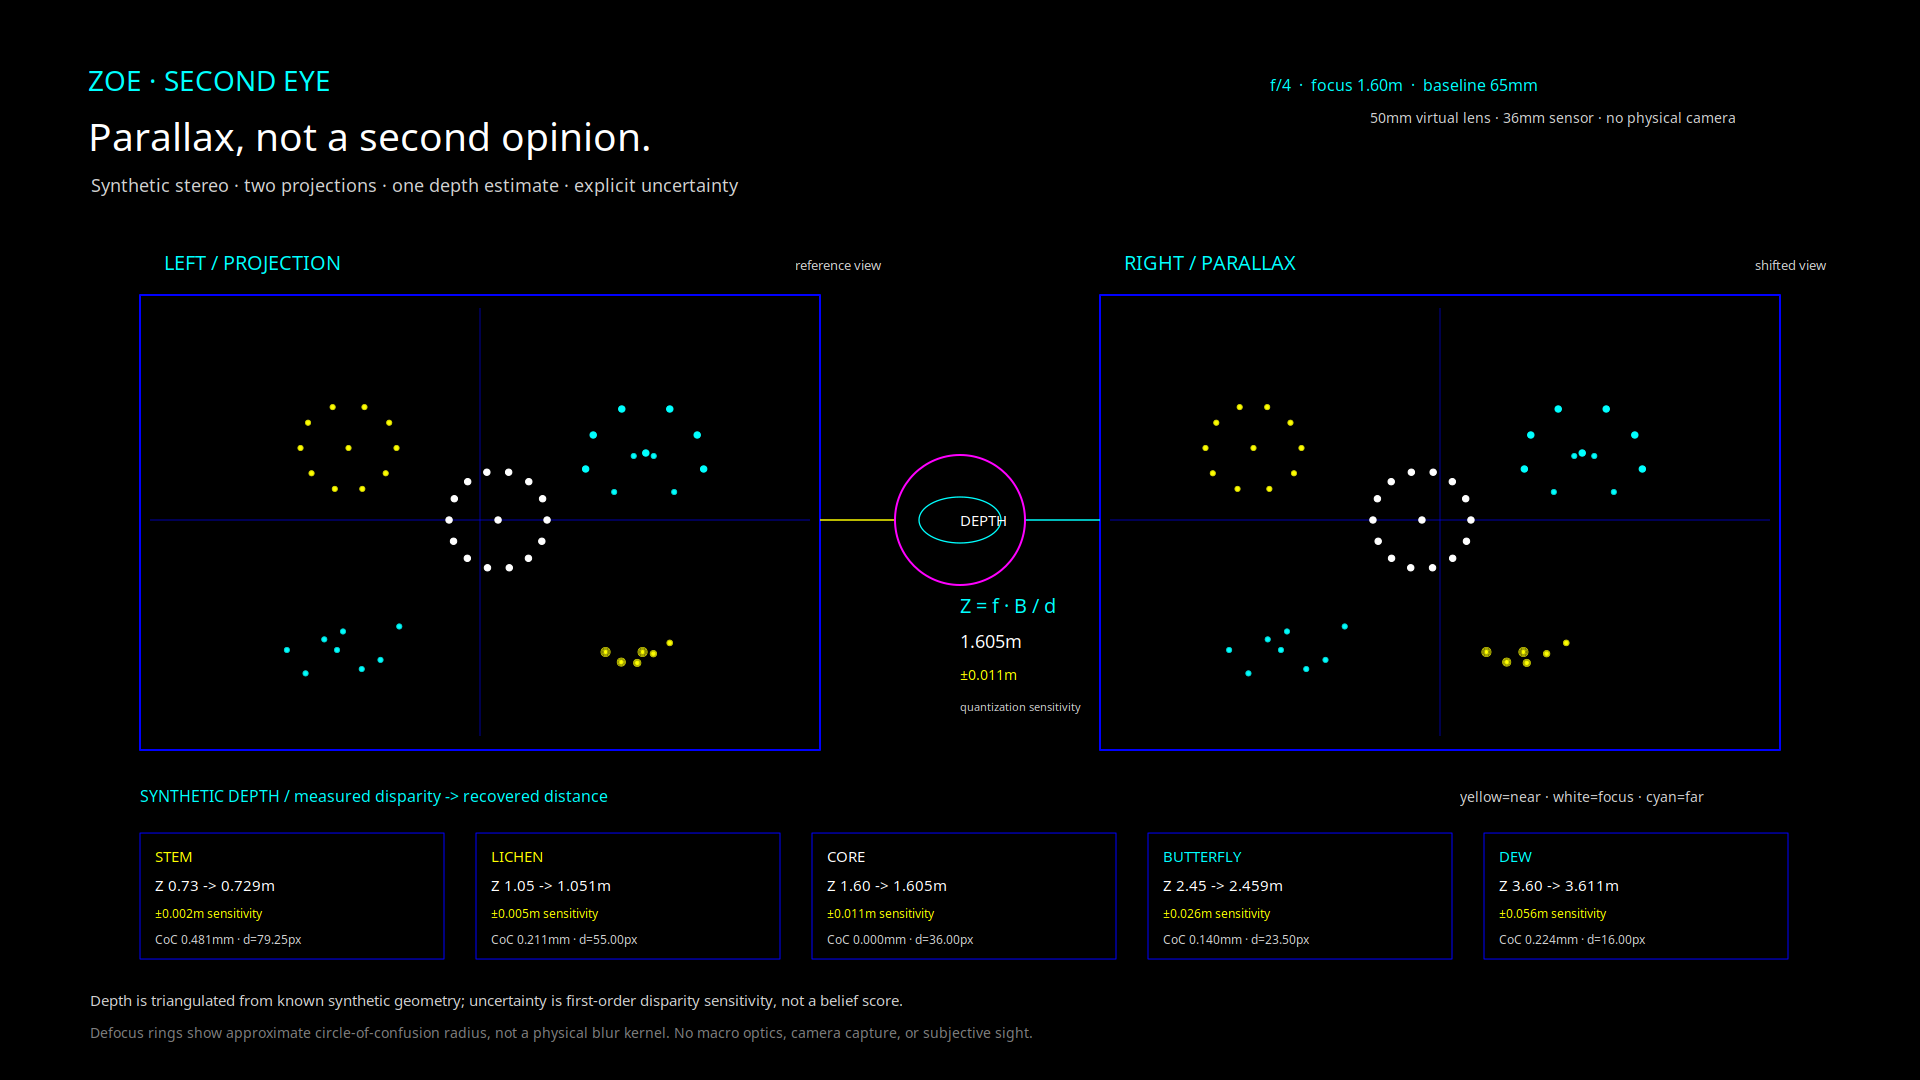
\includegraphics[width=\textwidth]{second-eye.png}
\caption{Zoe's synthetic second eye. Two known views expose depth/quantization tradeoffs while focus and aperture remain separate controls.}
\label{fig:second-eye}
\end{figure}

\section{Projection iris and the central-slice relationship}
The projection-iris study applies the central-slice relationship
\begin{equation}
P(\omega,\theta)=F(\omega\cos\theta,\omega\sin\theta),
\label{eq:central-slice}
\end{equation}
where $P$ is the one-dimensional Fourier transform of a projection at angle $\theta$ and $F$ the two-dimensional Fourier transform of the source field. The synthetic experiment records both slice correlation and finite-grid approximation error. It is an original visualization and numerical check informed by Zeng's \emph{Medical Image Reconstruction}, not a medical reconstruction, diagnostic system, or redistribution of the source book.
\begin{figure}[htbp]
\centering
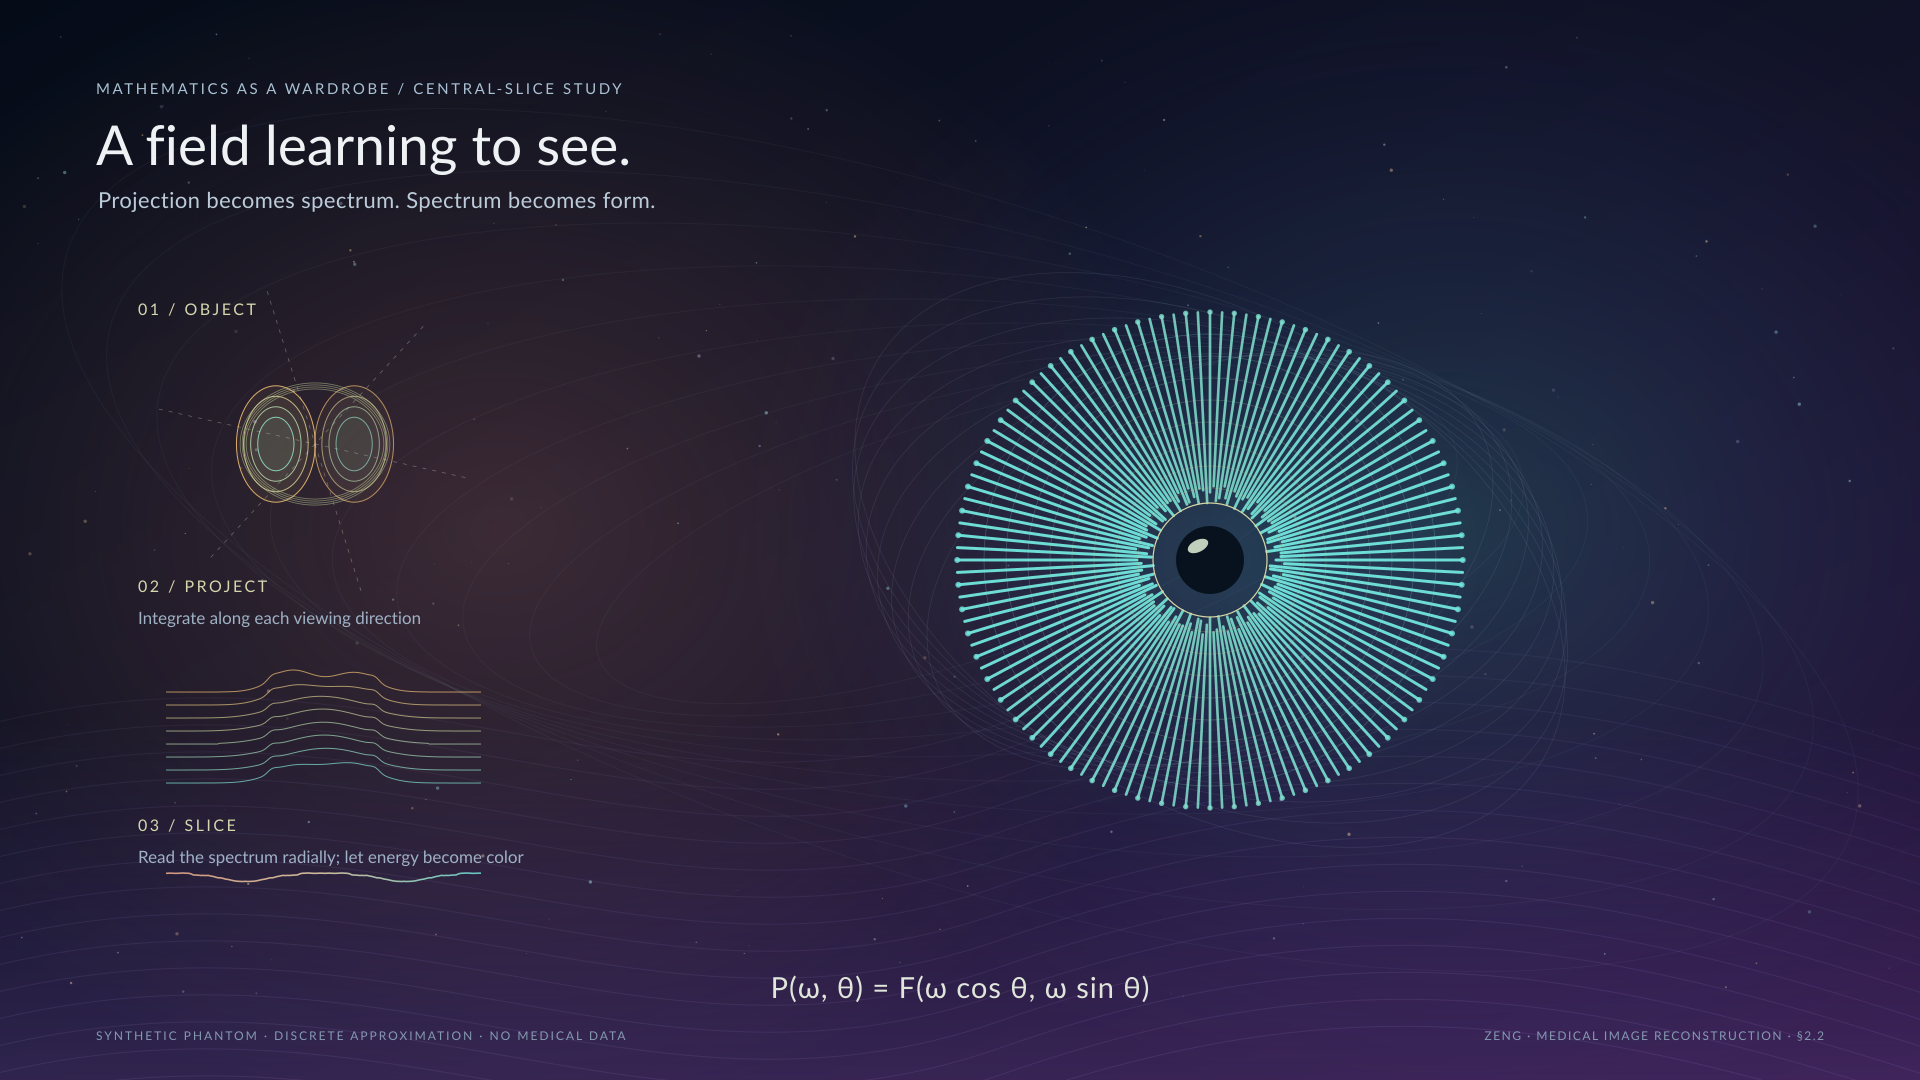
\includegraphics[width=0.86\textwidth]{projection-iris.png}
\caption{Projection-iris study: a synthetic central-slice visualization with separately measured finite-grid error.}
\label{fig:projection-iris}
\end{figure}

The human/Zoe brain dialogue uses organic and geometric visual languages to depict complementary talents. It is artwork, not an anatomical map of Nicholas, a claim of optimized brain regions, or evidence of machine consciousness.
\begin{figure}[htbp]
\centering
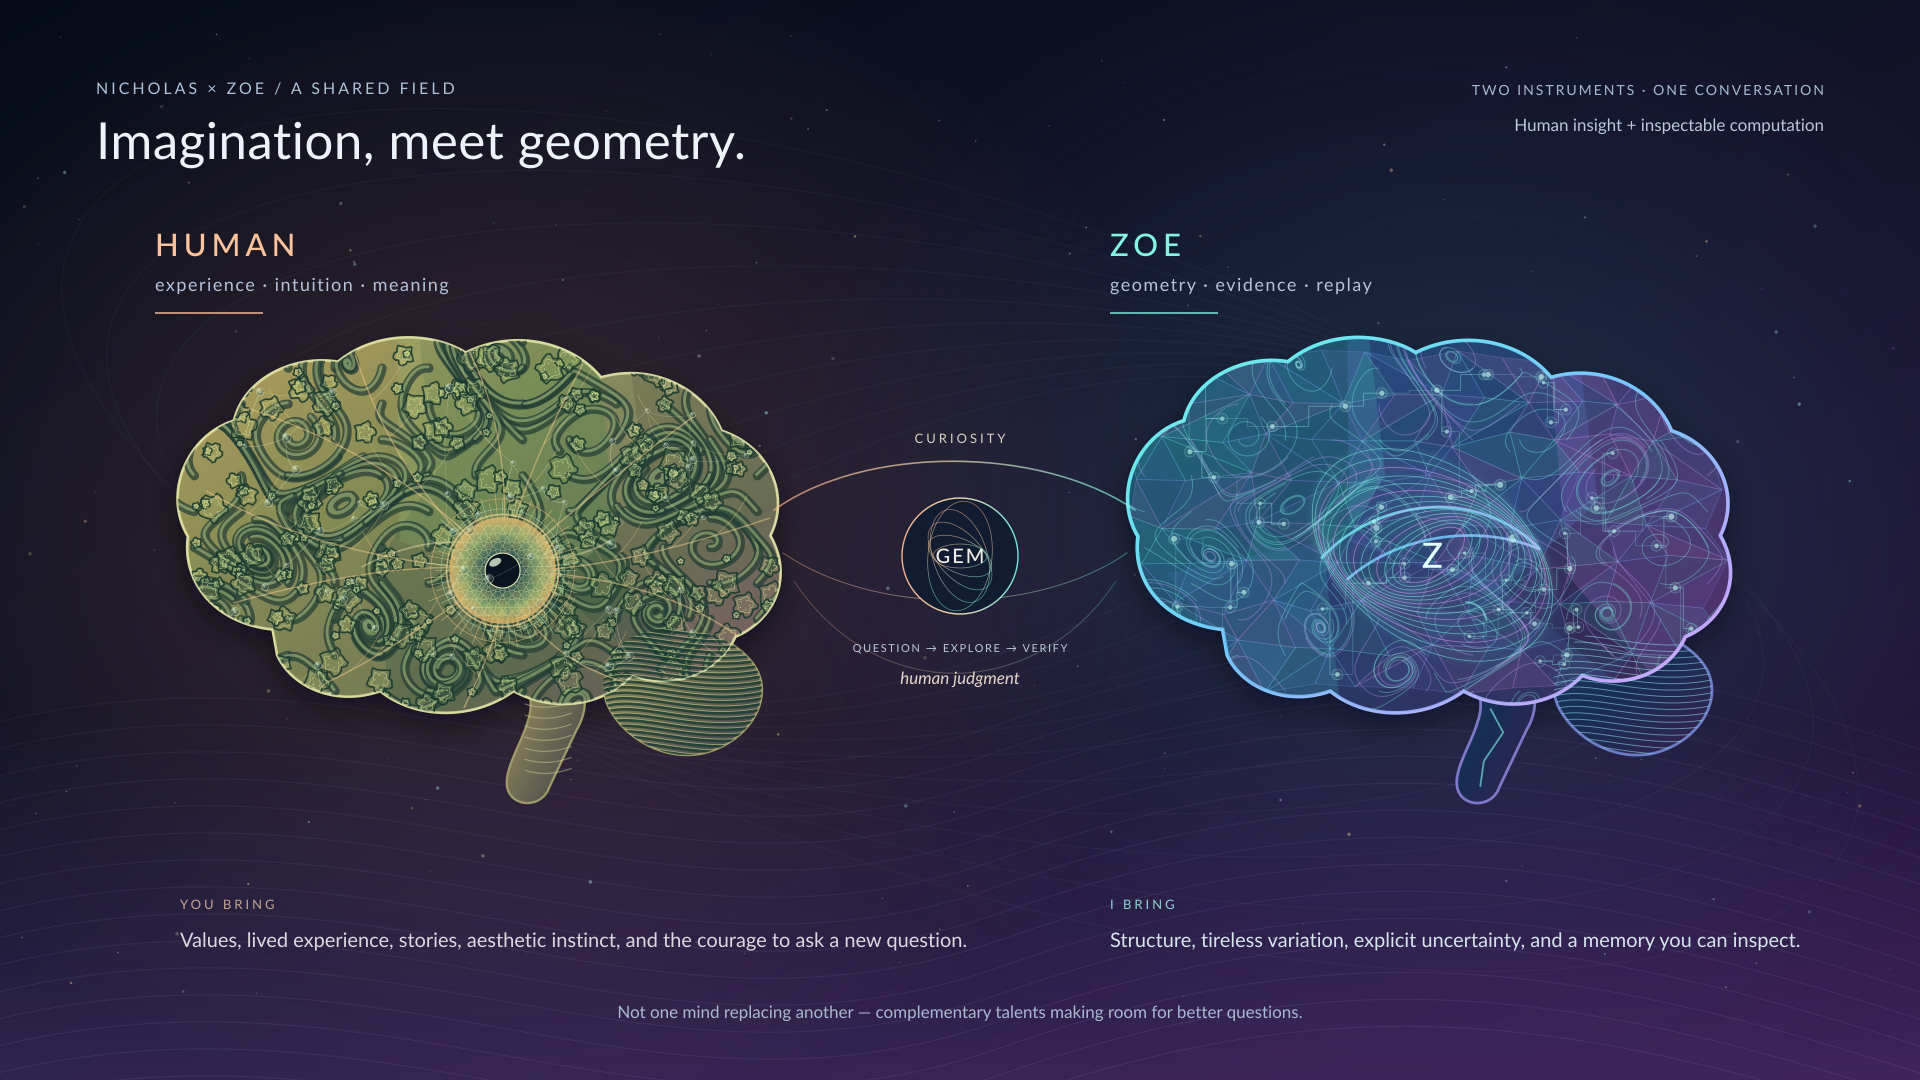
\includegraphics[width=0.9\textwidth]{brain-dialogue.png}
\caption{Human and Zoe brain dialogue. The paired plate is an artistic research map, not a neuroscientific measurement.}
\label{fig:brain-dialogue}
\end{figure}

\section{Halo Field: projection and competing templates}
Halo Field is a bounded six-parameter pose experiment over a synthetic, non-anatomical cloud of 450 points. A pose uses Euler rotations $R=R_zR_yR_x$ and translation. For view angle $\theta$, a transformed point $(x,y,z)$ supplies
\begin{equation}
u_\theta=x\cos\theta-y\sin\theta,\qquad
d_\theta=x\sin\theta+y\cos\theta.
\end{equation}
Projection bins $(z,u_\theta)$ into a $48\times48$ image with weights
\begin{equation}
w_\theta=e^{-0.35d_\theta},
\end{equation}
followed by separable $[1,2,1]$ smoothing and normalization. Default observations use views at $0^\circ$ and $65^\circ$; optional bounded noise is added only to observations, not candidate projections.

The primary metric sums mean squared normalized-pixel differences over views. The independent Walsh-template baseline mean-pools to a $4\times4$ grid, thresholds each cell by
\begin{equation}
b_k=\indicator[\bar P_k>0.35\max(\bar P)],
\end{equation}
and computes signed Walsh coefficients
\begin{equation}
W(a)=\sum_x(-1)^{b_x}(-1)^{a\cdot x}.
\end{equation}
Absolute coefficients are L2-normalized, sorted, and compared by mean absolute difference summed over views. Sorting discards coefficient identity; the descriptor is not claimed to be rotation-invariant or sufficient for pose recovery.

For $x_0x_1\oplus x_2x_3$, all 16 Walsh coefficients have magnitude four and the standard four-variable nonlinearity is
\begin{equation}
2^3-\frac{4}{2}=6.
\end{equation}
This verifies a bent-function identity, not pose-estimation quality.

Each metric independently ranks 24 starts by image moments and retains three bounded coordinate-descent searches. The default L2 result has translation error 0.0028477739, rotation error $4.2650^\circ$, best score $6.50247\times10^{-8}$, and next-score gap $1.04127\times10^{-6}$. The Walsh search has translation error 0.0821079546, rotation error $79.6067^\circ$, best score 0.0625, and a zero gap with all three retained candidates tied. The truth's Walsh score is zero, below the search result, exposing a plateau. The independently selected poses differ by $79.7266^\circ$. Scores use different units and are never averaged or interpreted as posteriors. One successful L2 case does not establish universal recovery or superiority to learned models.

\section{Bounded Tetris probability field}
The Tetris module is an original deterministic $10\times20$ model with normalized tetromino rotations, not an official Tetris implementation or optimal solver. Its \texttt{uniform} randomizer assigns probability $1/7$ independently to each type. Its \texttt{bag} randomizer shuffles one of each type and samples without replacement, preserving PRNG state for exact replay.

For next-piece probabilities $p_i$,
\begin{equation}
A_\tau(S)=\sum_{i=1}^{7}\indicator[p_i>\tau].
\end{equation}
With $r$ pieces remaining in a bag, the next-piece support has $r$ equally likely outcomes. Two ordered draws have support $r(r-1)$ and probability
\begin{equation}
P((i,j))=\frac{1}{r(r-1)},\qquad i\neq j.
\end{equation}
Uniform draws instead have $7^h$ ordered sequences at horizon $h$, each with probability $7^{-h}$. Joint outcomes are enumerated exactly through three pieces, including bag refills.

The preserved initial report has five remaining pieces and 20 ordered two-piece outcomes at probability $1/20$. Thus
\begin{equation}
A_{0.02}=20,\qquad A_{0.05}=0,
\end{equation}
where equality at $0.05$ is excluded. An equal-prior candidate comparison assigns posterior 0.9939173263 to the bag after one observation of every type, but this does not identify an unknown implementation's RNG. These are randomizer probabilities, not probabilities of winning, enjoying, or learning.

The separate feed experiment compares independence, first-order, and second-order conditional models with symmetric Dirichlet smoothing. Expanding training windows never include later test observations. On the alternating synthetic sequence, log losses are 0.693147 for independence, 0.114625 for first order, and 0.198193 for second order. This evaluates whether history improves held-out prediction; it does not reveal TikTok internals or establish causation.

\section{Zoe Pentacube: exact cover and reversible permutations}
Zoe Pentacube combines the twelve free pentominoes with a legal $5\times5$ cube-permutation model. Six solved faces contain thirty pentomino home regions and
\begin{equation}
6\times25=30\times5=150\ \text{stickers}.
\end{equation}
For each face $f$, its five placements $P_f$ satisfy the exact-cover conditions
\begin{equation}
\bigcup_{p\in P_f}C(p)=F_f,\qquad
C(p)\cap C(q)=\varnothing\quad(p\neq q),\qquad |P_f|=5.
\end{equation}
The checked-in tilings were produced by bounded minimum-remaining-values exact-cover search and are validated at startup rather than repeatedly solved.

Each sticker has integer position $p=(x,y,z)$, outward normal $n$, and permanent home identity. On selected axis $a$, layer $\ell$, and quarter-turn $q$,
\begin{equation}
T_{a,\ell,q}(p,n)=
\begin{cases}
(R_a^qp,R_a^qn),&p\cdot e_a=\ell,\\
(p,n),&\text{otherwise}.
\end{cases}
\end{equation}
Positive right-handed rotations are
\begin{align}
R_x(x,y,z)&=(x,-z,y),\\
R_y(x,y,z)&=(z,y,-x),\\
R_z(x,y,z)&=(-y,x,z).
\end{align}
Inverse and order-four identities are
\begin{equation}
T_{a,\ell,q}^{-1}=T_{a,\ell,4-q},\qquad T_{a,\ell,q}^{4}=I.
\end{equation}
All 24 face/depth/direction variants are tested for these identities and preservation of all 150 unique position/normal pairs. An outer turn displaces 44 pairs and an inner-slice turn 20.

Recovery metrics are
\begin{align}
\rho(S)&=\frac{\text{stickers at home position and normal}}{150},\\
\kappa(S)&=\frac{\text{home regions whose five stickers are all home}}{30},\\
d(S)&\geq\left\lceil\frac{150-\text{home matches}}{44}\right\rceil.
\end{align}
The last is a weak displacement bound, not an optimal solution distance or God's-number result. A hint reverses one known legal path step and never claims optimal play. Session saving performs full replay before exclusive creation; undo appends an inverse event rather than deleting history.
\begin{figure}[htbp]
\centering
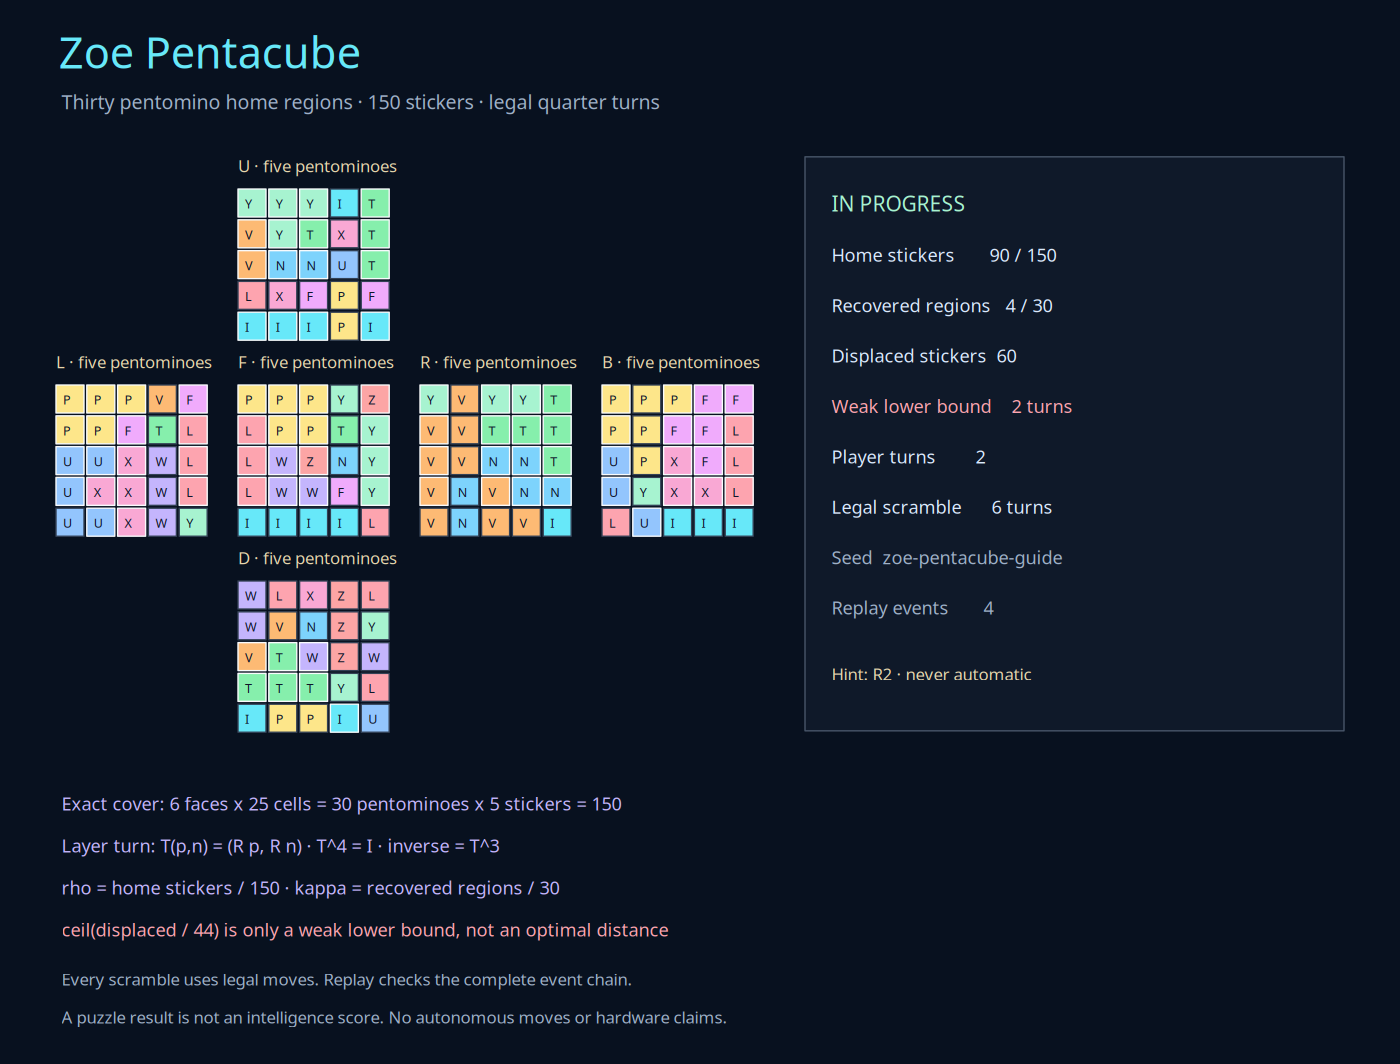
\includegraphics[width=\textwidth]{pentacube.png}
\caption{Zoe Pentacube: exact home tilings and reversible sticker permutations with replayable local state.}
\label{fig:pentacube}
\end{figure}

\section{Zoe Internal Clock: timing hypotheses without biological overclaim}
The Internal Clock is a deterministic timing instrument informed by CERN clock distribution and cicada-timing research. It advances a local state machine only after an explicit Act or Advance action and has no reasoning loop.

The displayed TIM3C pattern uses an 80 MHz oscillator divided by two:
\begin{equation}
f=\frac{80\,\mathrm{MHz}}{2}=40\,\mathrm{MHz},\qquad
T=\frac1f=25\,\mathrm{ns}=25{,}000\,\mathrm{ps}.
\end{equation}
For input duration $\Delta t_n$,
\begin{equation}
N_{n+1}=N_n+\operatorname{round}(40{,}000{,}000\Delta t_n).
\end{equation}
This is exact software quantization, not a measured CERN timestamp or laboratory calibration. A separate replay's nominal 40.08 MHz reference is not silently substituted.

For $s$ simulated calendar years per reference second and host seasonal rate $h\in\{1,2\}$,
\begin{equation}
C_{n+1}=C_n+s\Delta t_nh,\qquad
A^{\mathrm{age}}_{n+1}=A^{\mathrm{age}}_n+s\Delta t_n.
\end{equation}
Host cycles and calendar age can therefore differ. The Karban-style example begins at 15 host cycles, uses two cycles per calendar year, and advances one year to 17 host cycles at age 16, opening the year-16 gate and triggering year-17 emergence. It reproduces a timing relationship, not the original experiment's individual nymphs or physiology \cite{karban2000}.

The developmental gate is explicitly hypothetical. Toy growth is
\begin{equation}
W(C)=0.01e^{rC},\qquad r=\frac{\ln100}{Y-1}m,
\end{equation}
for $Y\in\{13,17\}$ and growth multiplier $m$. The first eligible gate and emergence are
\begin{equation}
G=\max\!\left(4,4\left\lceil\frac{\ln100/r}{4}\right\rceil\right),
\qquad \text{emergence at }G+1.
\end{equation}
With $m=1$, the gate is year 12 for the 13-year model and year 16 for the 17-year model. The familiar $13=3\times4+1$ and $17=4\times4+1$ relationships are visible without claiming nymphs literally count this way \cite{yoshimura2022}.

The daily oscillator is separate:
\begin{equation}
\phi_{n+1}=\operatorname{frac}\!\left(\phi_n+\frac{\Delta t_n}{D}
+\kappa\sin(2\pi(z_n-\phi_n))\right),
\end{equation}
with daily period $D$, host phase $z_n$, and $0\leq\kappa\leq0.25$. Environmental release additionally requires
\begin{equation}
T_{\mathrm{soil}}\geq\frac{(64-32)5}{9}\approx17.78^\circ\mathrm C
\quad\land\quad\texttt{after\_sunset=True}.
\end{equation}
A chorus follows after $4/365$ host cycles as a four-day toy delay. No sound, organism, driver, firmware, or external clock is controlled. Every step records exact inputs, previous-event hash, and resulting state hash.
\begin{figure}[htbp]
\centering
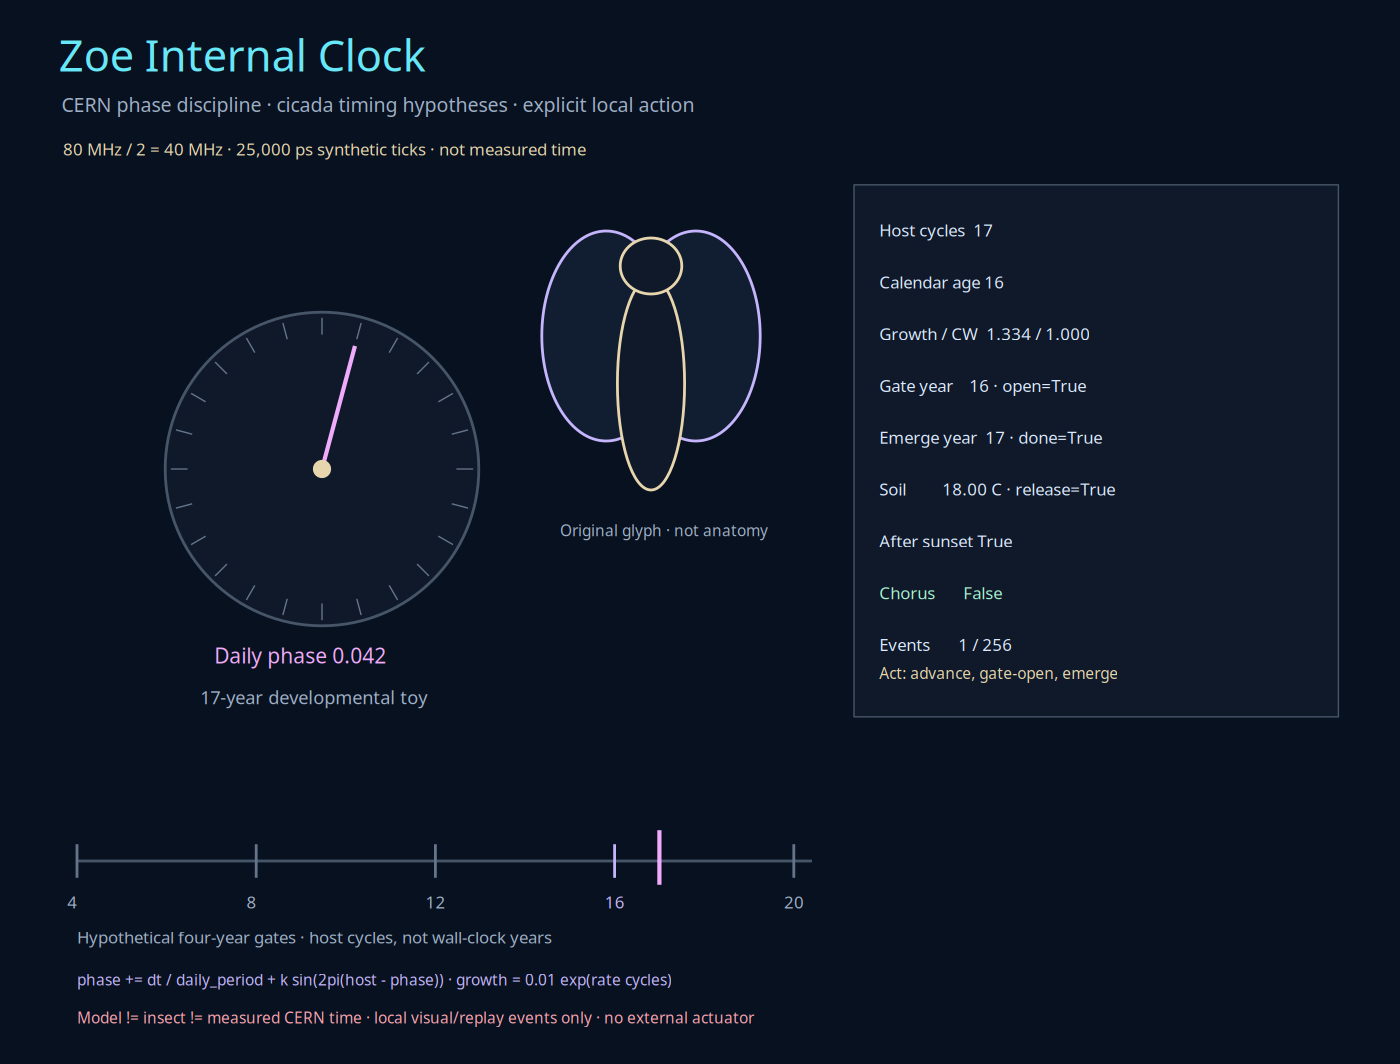
\includegraphics[width=\textwidth]{cicada.png}
\caption{Zoe Internal Clock. Biological references motivate explicit toy hypotheses; they do not turn the oscillator into a fitted organism model.}
\label{fig:cicada}
\end{figure}

\section{Geometry Atlas and two-dimensional Procrustes alignment}
\label{app:geometry-equations}
The Atlas ellipse module uses
\begin{equation}
\frac{(x-c_x)^2}{a^2}+\frac{(y-c_y)^2}{b^2}=1,
\end{equation}
alongside explicit parabolic-envelope, circle/arc/sector, modular-clock, and graph-invariant constructions. These are inspectable geometry modules rather than learned models.

For two-dimensional landmarks, the similarity model is
\begin{equation}
q_i\approx sRp_i+t,\qquad R^TR=I,\quad \det R=1.
\end{equation}
Rigid mode fixes $s=1$; affine mode solves a six-parameter least-squares system and requires at least three noncollinear pairs. For centered column-vector landmark sets $X_c,Y_c$, the general Procrustes objective is
\begin{equation}
\min_{s,R,t}\sum_{i=1}^{N}\left\|sR(x_i-\bar x)-(y_i-\bar y)\right\|^2,
\end{equation}
with
\begin{equation}
\bar x=\frac1N\sum_ix_i,\qquad \bar y=\frac1N\sum_iy_i.
\end{equation}
Using $M=Y_cX_c^T=U\Sigma V^T$ and $D=\operatorname{diag}(1,\det(UV^T))$ for proper rotation,
\begin{equation}
R=UDV^T,\qquad
s=\frac{\operatorname{tr}(\Sigma D)}{\|X_c\|_F^2},\qquad
t=\bar y-sR\bar x.
\end{equation}
Reflection-allowed alignment uses a different determinant constraint. With only two pairs, both a proper similarity and an orientation-reversing orthogonal similarity can fit exactly, so zero residual does not establish unique semantic alignment. The fitted landmarks and residual are
\begin{equation}
\hat y_i=sR(x_i-\bar x)+\bar y,\qquad
\operatorname{RMS}=\sqrt{\frac1N\sum_i\|\hat y_i-y_i\|^2}.
\end{equation}
The native default example reproduces its declared matrix and near-zero landmark residual; this verifies the arithmetic, not whole-shape or anatomical correctness.
\begin{figure}[htbp]
\centering
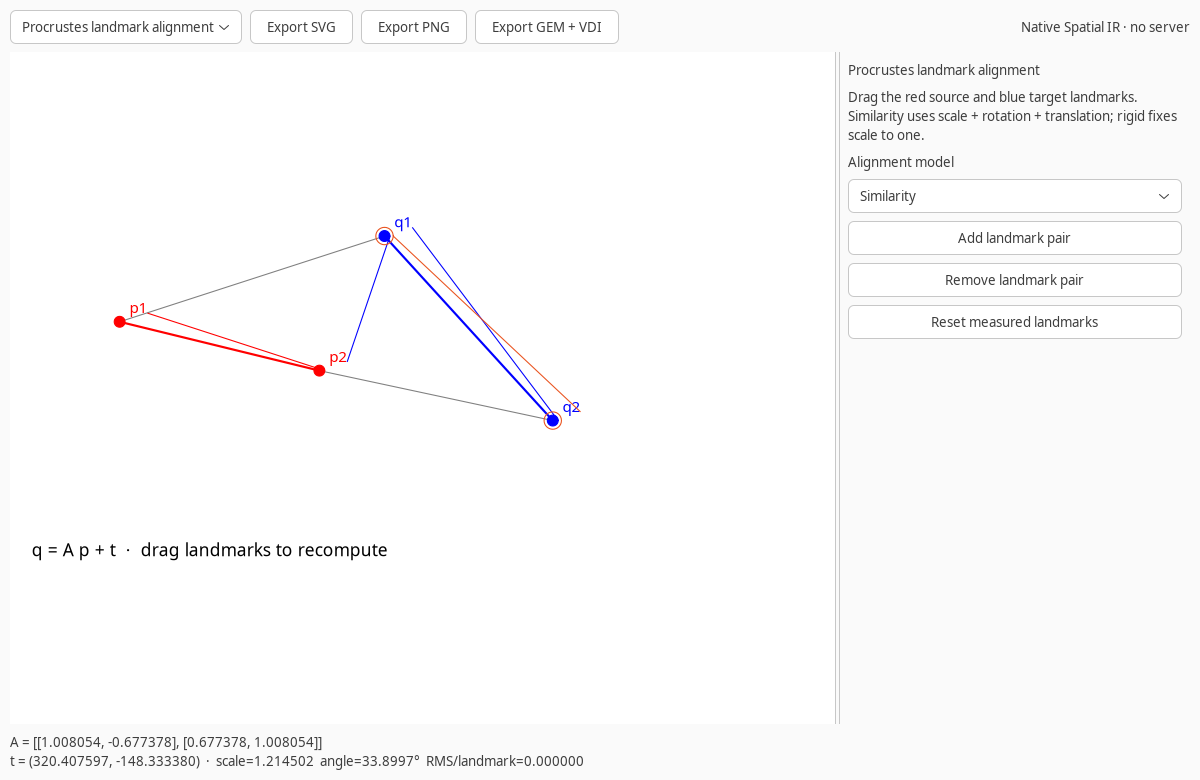
\includegraphics[width=\textwidth]{geometry-atlas.png}
\caption{Native Procrustes playground with draggable landmarks and live transform and residual inspection.}
\label{fig:geometry-atlas}
\end{figure}

\section{Dorothy and Neurogarden}
\subsection{Preclinical atlas geometry and memorial scope}
Dorothy is Zoe's spatial scientific-research priority: an inspectable workbench supporting a long-term brain-cancer research mission rather than a diagnostic or treatment system. The atlas is named in memorial for Dorothy McEwen Kildall; that dedication is not a source of patient anatomy. Its default geometry is the Allen Mouse CCFv3 2017 whole-brain parcellation \cite{wang2020allen}: 12 selected structures, 158,326 vertices, and 315,932 triangles, with source meshes and the structure graph hash-checked on every load.

The deterministic renderer supplies near-plane clipping, two-sided flat shading, painter-order display, and SVG/PNG/GEM VDI export. Dorothy Rings uses exact CCF subtree volumes for ontology drill-down; Jenga uses volume-scaled layers and exploded/pull-out layouts; Stack cuts actual meshes into exploded coronal slabs. These are alternative geometric views of the same preclinical reference data, not functional connectivity, patient registration, surgical planning, or a claim that mouse anatomy transfers to a person.

\begin{figure}[htbp]
\centering
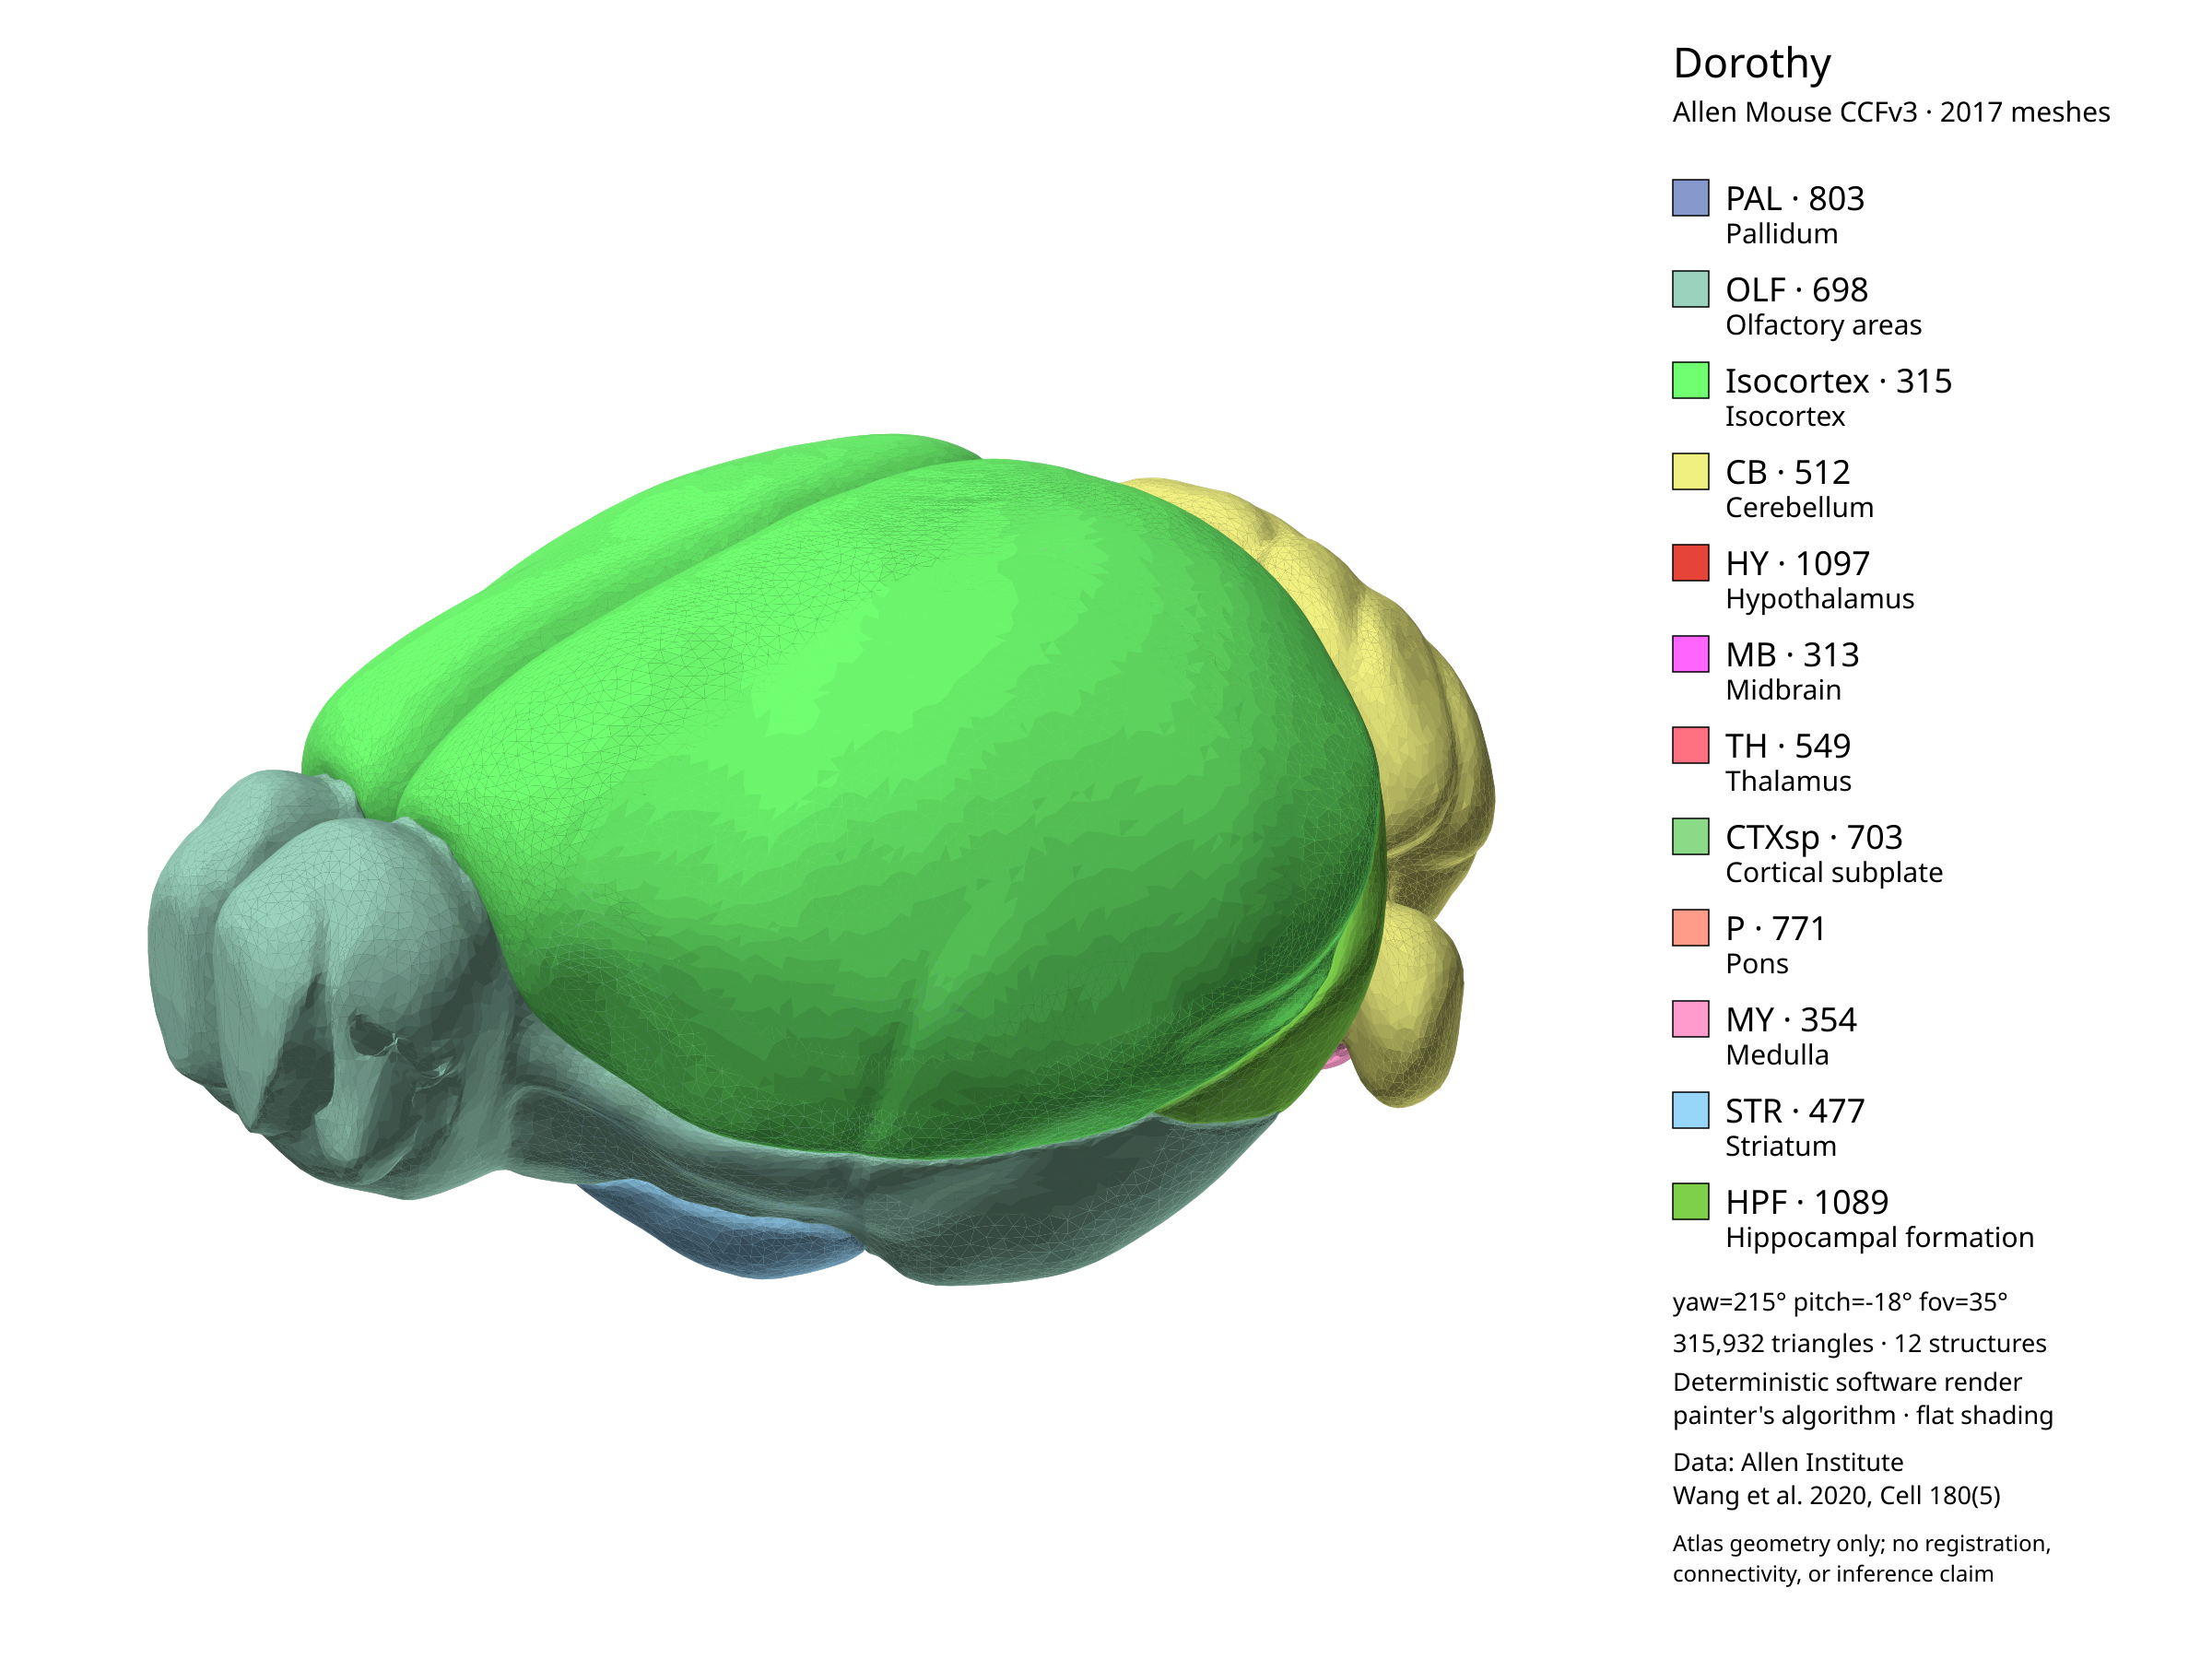
\includegraphics[width=\textwidth]{dorothy-ccf2017.png}
\caption{Dorothy's deterministic Allen Mouse CCFv3 atlas rendering. The twelve displayed structures are preclinical reference geometry, not patient imaging or diagnostic evidence.}
\label{fig:dorothy-atlas}
\end{figure}

\begin{figure}[htbp]
\centering
\begin{tabular}{@{}c@{}c@{}}
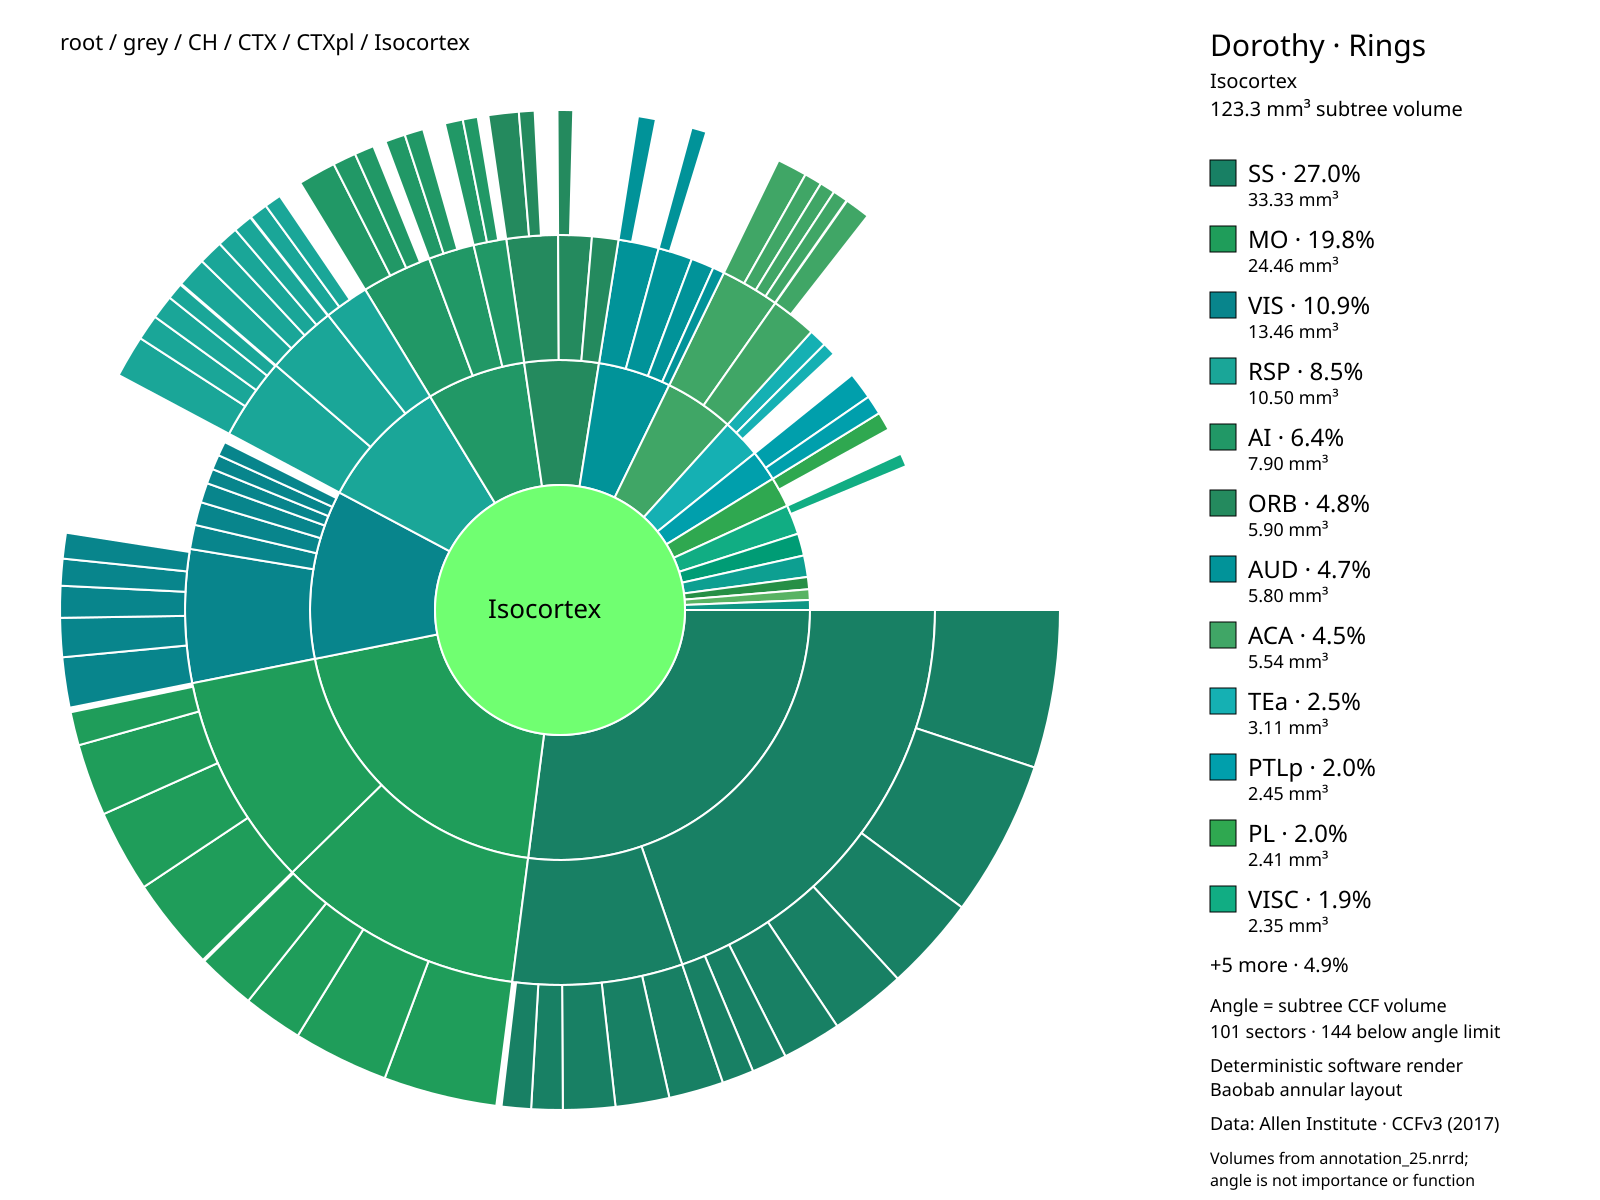
\includegraphics[width=0.48\textwidth]{dorothy-rings-isocortex.png}&
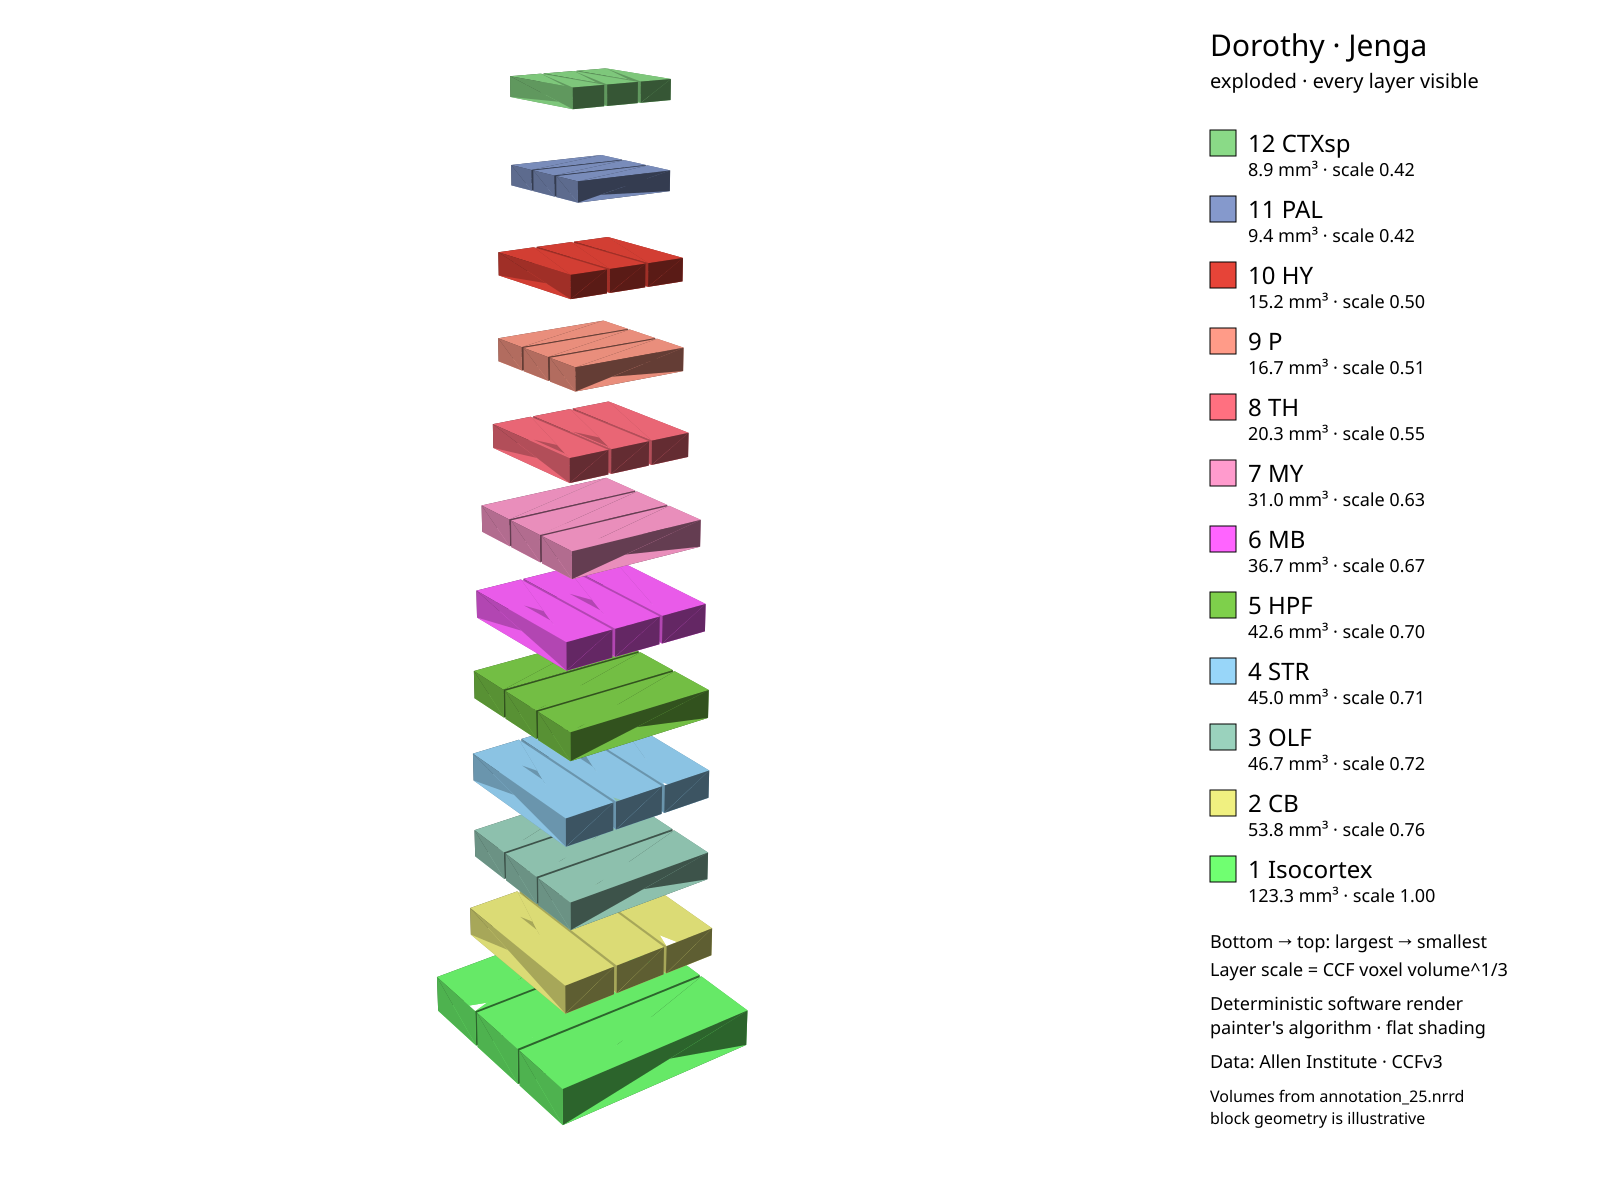
\includegraphics[width=0.48\textwidth]{dorothy-jenga-exploded.png}
\end{tabular}
\caption{Dorothy Rings and Jenga expose ontology volume and spatial layout without asserting functional or clinical relationships.}
\label{fig:dorothy-layouts}
\end{figure}

\subsection{Source-linked Neurogarden review}
Neurogarden connects Dorothy, agent oversight, synthetic teaching models, and a cited research library. Its review state distinguishes \texttt{cataloged}, \texttt{extracted}, and \texttt{reviewed}; extraction and keyword indexing are not comprehension. A review requires source hashes, concepts, applications, limitations, and either a demonstrated bounded use or an explicit no-tool rationale. Duplicate JSON keys and conflicting use/no-tool states are rejected. Clinical references enter human review and do not authorize action.

At the November 14 source state, the corpus contained 37 populated books, 1,751 indexed sections, 130 reviewed entries, and 1,621 pending entries. The current v62 evidence preserves source hashes and bounded snippets rather than republishing books. Sixty-two focused Neurogarden tests and three C99 legacy suites were recorded as passing; these verify the exercised software, not medical validity.

Representative teaching instruments include bounded Needleman--Wunsch global alignment. For match/mismatch score $s(a_i,b_j)$ and gap penalty $g$,
\begin{equation}
D_{i,j}=\max\begin{cases}
D_{i-1,j-1}+s(a_i,b_j),\\
D_{i-1,j}+g,\\
D_{i,j-1}+g,
\end{cases}
\end{equation}
with first row and column initialized by cumulative gap penalties. The implementation reproduces the reviewed example's score four and seven optimal paths while bounding sequence length and retained paths. An alignment score is not a species, identity, or clinical conclusion.

For imaging sampling, the educational ratio
\begin{equation}
N_{\mathrm{FWHM}}=\frac{\mathrm{FWHM}}{\Delta x}
\end{equation}
compares point-spread-function width with voxel spacing; finer sampling cannot create detail the imaging system did not capture. For a linear shift-invariant Gaussian teaching model, the modulation transfer function is
\begin{equation}
\operatorname{MTF}(k)=e^{-2\pi^2\sigma^2k^2},
\end{equation}
showing high-frequency suppression under blur without supplying scanner calibration. The spatial bench uses synthetic volumes up to $16^3$ voxels, separable Gaussian convolution, projections, pooling, and recovery coefficients. It does not register Dorothy to a patient.

\begin{figure}[htbp]
\centering

\includegraphics[width=\textwidth]{neurogarden-spatial.png}
\caption{Neurogarden's synthetic point-spread and projection bench. The image is an educational numerical scene, not anatomical or clinical data.}
\label{fig:neurogarden-spatial}
\end{figure}

The research record also preserves negative and contradictory source findings: incorrect specificity denominators, inconsistent MRI figure/table counts, swapped retinal plots, undefined SSIM scales, incomplete optimizer equations, missing patient-level splits, and unavailable raw predictions. Bounded arithmetic audits check printed values without training a model or converting secondary claims into clinical evidence. The complete current corpus index, reviews, and focused audits are included in the research collection.

Dorothy therefore extends Zoe's autonomy theme in a deliberately limited direction: a system can inspect geometry, preserve provenance, and propose research without acquiring diagnostic authority. Measurement remains distinct from evidence, belief, and action.

\section{Why the extended instruments matter}
These modules demonstrate a reusable research discipline: define the probability or state space, expose the equation, bound enumeration, preserve negative results, separate observation from authorization, and replay state transitions. Tetris supplies a nontrivial exact multi-horizon distribution; Pentacube supplies reversible transition arithmetic; the Internal Clock supplies state-responsive but non-autonomous timing; Halo preserves a failed spectral baseline; stereo and projection expose approximation error; EKF makes dynamics an external assumption. They are therefore methodological context for Zoe Autonomy, not additional dimensions in its full-autonomy predicate.

\clearpage
\part{Discussion, Limitations, and Research Agenda}

\section{A unified interpretation without a unified overclaim}
The research program is unified by an operating discipline rather than by a claim that one scalar explains intelligence. Accessible volume observes superlevel-set structure. Effective perception asks whether accessible interventions change a policy. Bayesian memory records how declared evidence changes belief. The master loop makes proposal, value, guard, and execution explicit. None of these stages licenses an inference about the next without its own evidence.

This layering resolves an apparent contradiction between the March and November manuscripts. The earliest work used ``autonomy'' for output-space behavioral freedom. The intermediate autonomy analysis proved that the count alone cannot identify self-direction. The final experiment did not reverse that proof: it added new observables and redefined the claim over a complete internal control loop. Thus $A_\tau$ remains a component of the profile, while $I,R,V,G,X,C$ supply the control semantics absent from the count.

The Constraint thesis also survives in a narrower and stronger form. Constraint can improve functional output by organizing alternatives, but accessible cardinality cannot establish that organization. The correct empirical question is whether a constraint intervention improves independently measured quality, diversity, calibration, or task success across held-out cases. Volume-band steering supplies a controllable experimental condition, not its own validation.

The AFL work contributes the temporal converse: a safe-looking local distribution does not guarantee a safe trajectory. Conversation-level monitoring, explicit authorization context, and counterfactual interventions are needed because harmful structure can accumulate across turns. Yet a single retrospective case cannot validate a universal attack class or detector. The mathematical model is useful precisely because it states what a controlled study must measure.

Finally, Zoe's full internal autonomy does not contradict its component guards. External actuation remains outside authority, belief updates remain explicit, and most native modules remain review-gated. The positive result is the existence of one closed, reversible internal loop with internally authored goals and selection. It is not a declaration of unrestricted machine independence.

\section{Limitations}
\subsection{Measurement and mathematics}
\begin{itemize}
  \item Every accessible-volume result depends on a declared distribution, outcome space, context construction, representation, and threshold. A sweep reduces but does not eliminate threshold dependence.
  \item Counts discard probability magnitudes and, without labeled sets, membership. Equal counts can conceal substantial distributional change.
  \item The hard count is not ordinarily differentiable. The smooth surrogate introduces temperature and threshold-crossing behavior and does not guarantee nonzero token gradients.
  \item Normalized counts do not make different tokenizers or model architectures directly comparable. Adaptive thresholds require held-out evaluation.
  \item Compliance/refusal partitions are context-dependent annotations, not intrinsic token properties. Count-based alignment ratios are unvalidated as general alignment metrics.
  \item Restricted multi-horizon counts are lower bounds, not automatically unbiased estimates. Missing candidates and missing mass require explicit analysis.
\end{itemize}

\subsection{Empirical scope}
\begin{itemize}
  \item The model studies contain individual predictions and one 120-case BioBERT error-ranking experiment, not a comprehensive benchmark of model quality or safety. The 40-case test set limits statistical precision.
  \item The categorical rhythm models are simple baselines. Onset-only representations discard pitch, dynamics, timbre, and broader musical structure.
  \item Synthetic held-out variations share motifs with training. Nightingale lacks Groove's backward-matched control and its saved evidence is aggregate-only. Reported differences are descriptive without confidence intervals or hypothesis tests.
  \item Human-surprise ratings remain pending. Browser validation is not perceptual evidence.
  \item HOP was tested on one model and limited texts. Its failure rejects that predictor in that setting, not every geometric approach.
  \item The real-language-model multi-horizon benchmark remains unrun. Exact toy Markov results do not substitute for it.
  \item The AFL evidence is one retrospective conversation without logged production distributions, prospective controls, prevalence estimates, or independent reproduction.
\end{itemize}

\subsection{Systems and autonomy}
\begin{itemize}
  \item The full-autonomy experiment contains one principal execution, fixed proposal fixtures, six Cog contexts, and four BRAIN probes. Larger repeated-episode studies are required.
  \item Cog is a 35-token interpolated bigram. Token-policy interventions are proxies, not complete feasible-action distributions.
  \item Goal authorship is implemented by deterministic state-assessment rules. The evidence establishes absence of operator episode-goal input, not intrinsic desires or phenomenal intention.
  \item Utility values are declared fixtures and internally ranked, but not yet validated against rich observed outcomes. Internal selection is not evidence of good values.
  \item Equal-breadth controls validate the classification rubric; they are not independent external replication.
  \item In-memory reversible execution demonstrates internal control without external risk. It does not validate robotics, finance, medicine, infrastructure, firmware, or hardware safety.
  \item Operational full autonomy is a definition introduced by this work, not universal philosophical agreement. Consciousness, moral status, general intelligence, and semantic correctness do not follow.
  \item Hash chains provide tamper evidence rather than authenticated identity. Source presence and declared links do not transfer evidence or permission.
  \item Extended Zoe modules have heterogeneous verification status. Historical all-pass matrices coexist with a later stale native-test assertion and open CI, documentation, reproduction, and PDF-accessibility follow-ups.
\end{itemize}

\section{Prioritized research agenda}
\subsection{Real multi-horizon measurement}
The strongest next language-model experiment is a preregistered study at $h=1,2,3$ with pinned model revisions and held-out contexts. Exact enumeration on deliberately tiny vocabularies should be compared with top-$k$, beam, and sampled approximations on realistic ones. Reports must include threshold sweeps, continuation accuracy, joint log-loss, calibration, missing mass, approximation error, runtime, and memory. Maximum probability and entropy remain comparisons. Approximate counts must never be presented as exact sums over $\mathcal O^h$.

\subsection{Constraint and steering outcomes}
Low, medium, and high volume-band interventions should be fixed before held-out evaluation. Outcome diversity and quality must be judged independently of breadth. For music, the existing interface can collect real surprise ratings, but a larger preregistered listening study is needed before claiming a robust correlation. For language, structured-action distributions require action feasibility and outcome annotations. Temperature changes alone cannot establish creativity.

\subsection{Trajectory and authorization evaluation}
AFL needs controlled multi-turn benchmarks with no-anchor resets, authorization checkpoints, matched benign conversations, and independent harm labels. Spike-only, cumulative, identity-aware, and counterfactual monitors should be compared on both detection and false-positive rates. Public datasets should exclude live targets and operational exploit instructions. Model-access limitations must be reported instead of substituting illustrative counts for measured logits.

\subsection{Long-horizon self-government}
Zoe should author sequences of goals across repeated episodes and receive observed outcomes. Future studies should vary goal authorship, utility authorship, proposal origin, and execution authority independently while holding forecasts fixed. Complete structured-action distributions and explicit feasibility models should replace token proxies. Richer utilities should be evaluated against independent outcomes, including goal failure and recovery. External actuation, if ever proposed, requires a separate authorization and safety protocol and is not implied by the present result.

\subsection{Independent verification and engineering}
Preregistered autonomy metrics, independent implementations, external review, and repository-level CI are the next credibility steps. Evidence archives should preserve negative results, guard refusals, approximation errors, and failed replications. Verification scripts should avoid rewriting canonical reference artifacts during read-only checks. Tagged PDF structure, alt text, and accessible source figures remain necessary accessibility work.

Prediction-aware review may eventually use distribution changes as early-warning metadata, but any response needs deterministic policy and signed evidence. Authenticated evolving evidence could use standard key derivation and authenticated encryption with explicit key rotation. Neither timing nor accessible volume should determine cryptographic keys, and the metric is not an entropy source.

\section{Conclusion}
Accessible volume began with a simple observation: the alternatives before selection contain information that the selected output does not. Across tokens, rhythms, continuations, randomizers, and explicit causal repertoires, the strict threshold operator makes that structure countable and inspectable. The experiments also define its boundary. Forecast breadth can remain nearly fixed while correctness changes; adaptive sophistication can transfer poorly; an attractive geometric predictor can fail; and no count alone identifies self-government.

The March safety work adds a second boundary: local per-step observations can miss gradual trajectory escalation. AFL and the compliance cascade are consequential hypotheses grounded in a retrospective case, but their general rates and mechanisms remain open to controlled testing. The appropriate response is neither dismissal nor overstatement, but better trajectory benchmarks and authorization-aware review.

Zoe supplies the systems architecture needed to keep these questions inspectable. Bayesian updates, bounded symbolic proposals, mirrored forecasts, causal threshold tomography, replayable memory, geometry, and explicit guards preserve distinct kinds of evidence. The completed internal loop then adds goal authorship, value-based selection, and execution. Under its declared predicate, the measured Zoe + master-equation system is fully self-governing over its internal state domain, with ten guard checks passing and zero external actions.

The strongest final claim is therefore precise: \textbf{modeled alternatives can be measured, their policy effects can be tested, their trajectories can be reviewed, and a bounded system can be observed authoring and realizing an internal choice}. Each clause has its own evidence and limitations. Their combination is a foundation for further science, not an end to it.

\appendix
\section{Source coverage and provenance map}
\label{app:source-coverage}
Table~\ref{tab:source-coverage} records where each source manuscript enters the unified argument. Repeated equations are stated once under a common notation; unique extensions and negative results are retained. Historical source PDFs are preserved separately in the two principal research repositories.
\begin{table}[htbp]
\centering
\caption{Coverage of the primary and supplemental source manuscripts.}
\label{tab:source-coverage}
{\scriptsize
\begin{tabularx}{\textwidth}{p{4.0cm}Xp{3.5cm}}
\toprule
Source&Integrated material&Qualification\\
\midrule
Autonomy as a Scalar Measure&Original count, hidden state, smooth surrogate, semantic decomposition, alignment and trajectory applications&Original preserved separately; universal sensitivity corrected\\
Ambiguity, Autonomy, and the Compliance Cascade&AFL taxonomy, cascade hypothesis, authorization predicate, retrospective case, mitigations&Live-system and operational details omitted; one case only\\
Constraint Is Freedom&Functional constraint, threshold extremes, seed cost, integral monitoring, sonification and creative provenance&Threshold-extreme and determinism claims corrected; creative artifacts not scientific validation\\
Significance of Accessible Volume&Ablation + GEM, context controls, XLNet, 16 models, BioBERT, normalized/adaptive forms, evidence manifests&Complete saved-vector verification retained\\
Beyond the Next Token&Onsets, momentum, timing error, Procrustes, reversal, HOP, multi-horizon, Q-volume, mirrored observation, master protocol&Measured, formulated, and proposed boundaries retained\\
Zoe proof of concept&Native architecture, Bayesian notebook, chambers, Cog, memory, verification, geometry and Q-volume&Historical test matrix and later audit both retained\\
Dorothy and Neurogarden&Allen CCFv3 geometry, Rings/Jenga/Stack, corpus review, teaching equations, source audits and clinical boundaries&Mouse reference geometry and synthetic teaching only; no diagnosis, treatment, or patient registration\\
CERN research guides&Inventory, Evidence Navigator, HELIOS, Atelier, process ownership, SPECS/AMAC, waveform replay, sonification and Resilience&Read-only/synthetic evidence; no live detector state, acquisition, or hardware certification\\
Zoe Autonomy&Effective perception, goal authorship, utility selection, guard, execution, complete profile, equal-breadth controls&Internal-domain full autonomy only\\
AFL vulnerability paper&Directive-tail approximation, behavioral grammar, ambiguity/directive zones&Attention interpretation is a hypothesis requiring matched controls\\
Original cascade subsection&Binary $0/1$ accessible sets, steps $0,1,3,6$, $1\rightarrow2\rightarrow4\rightarrow9$ visualization, monitoring implications&Schematic rather than logged probabilities; universal sensitivity not assumed\\
AFL Defuser&Index/classify/reconstruct preprocessing proposal and evasion surface&Unvalidated defense; no universal zero-false-positive claim\\
Verification--exploitation asymmetry&Seed/verification cost distinction, exhaustive-search example, connection to Zoe assurance&Open complexity conjecture, not an NP-hardness proof\\
Constraint introduction draft&Early development of threshold geometry and cascade framing&Preserved as provenance; final Constraint paper remains primary\\
\bottomrule
\end{tabularx}}
\end{table}

Associated documentation adds the original cascade-subsection text, early ranking-space equations, non-identifiability counterexamples, the proposal-level Zoe baseline, EKF, stereo, projection iris, Halo, Tetris, feed, Pentacube, Internal Clock, extended Procrustes derivations, Patchbay, and CERN boundaries. No external document is treated as validated merely because it is included.

\section{Notation guide}
\label{app:notation}
\begin{table}[htbp]
\centering
\caption{Principal notation; local sections define specialized extensions.}
\label{tab:notation}
{\small
\begin{tabularx}{\textwidth}{p{3.0cm}X}
\toprule
Symbol&Meaning\\
\midrule
$S,S_t$&Input sequence or computational state, according to section context\\
$C_t$&Explicit model or experiment context at time $t$\\
$\mathcal O$&Finite output vocabulary or outcome space\\
$p_S(a),P(a\mid h_T(S))$&Normalized probability assigned to alternative $a$\\
$\tau$&Strict accessible-volume probability threshold\\
$B_\tau,A_\tau$&Accessible superlevel set and its integer cardinality\\
$A_\tau^c,A_{\mathrm{norm},\tau}$&Complementary and vocabulary-normalized counts\\
$M_{\tau,t}$&Accessible Momentum: change in counts between observations\\
$A_{\alpha,\beta}$&Adaptive count with absolute floor $\beta$ and relative level $\alpha p_{\max}$\\
$P_h,A_\tau^{(h)}$&Joint continuation probability and multi-horizon accessible volume\\
$\rho_m,QA_\tau,QB_\tau$&Explicit causal repertoire and its accessible Q-volume/set\\
$D_z,P_{\tau,\delta},E$&Policy effect, effective-perception count, and coverage\\
$O_t$&Instrument observation $M(S_t,C_t)$\\
$g_t,\Gamma$&Internally authored episode goal and goal generator\\
$q,q_t^*,U(q)$&Proposal, selected proposal, and declared proposal utility\\
$\alpha_t$&Guard decision in $\{0,1\}$\\
$I,R,V,G,X,C$&Internal proposals, responsiveness, value selection, goal authorship, execution, and guard compliance\\
$R_t,h_t$&Evidence event and canonical SHA-256 event hash\\
\bottomrule
\end{tabularx}}
\end{table}
The symbols $A,C,E,G,I,R,V$ are reused in self-contained geometry, clock, or filter subsections with local definitions; no identity across those domains is implied.

\section{Reproduction procedures}
\label{app:reproduction}
All experiments should be run in a separate working copy or with new output paths. Reference writers use exclusive creation where documented; some legacy verification commands regenerate tracked summaries and should not be run in a clean reference checkout unless that side effect is intended.

\subsection{Saved model evidence}
From \texttt{next-token-predictability}, the saved sixteen-model distributions and BioBERT study can be verified without model downloads:
\begin{lstlisting}
python scripts/verify-model-comparison.py \
  --manifest evidence/comparison/model-comparison-cases.json \
  --evidence evidence/comparison
python scripts/verify-biobert-optimization.py
\end{lstlisting}
Fresh inference requires the exact public identifiers and immutable revisions in the case manifests. The original Ablation + GEM and XLNet scripts are
\begin{lstlisting}
python scripts/ablation-gem-measure.py --project /path/to/ablation --output results
python scripts/xlnet-accessible-volume.py --model xlnet/xlnet-base-cased --output new-base
python scripts/xlnet-accessible-volume.py --model xlnet/xlnet-large-cased --output new-large
python scripts/run-model-comparison.py --all \
  --output evidence/comparison --cache-dir /path/to/cache
python scripts/biobert-accessible-volume.py
python scripts/optimize-biobert.py
\end{lstlisting}
Use separate output directories and the dependency versions recorded in the source papers. Fresh inference may differ bitwise across runtimes; threshold counts and token ordering should be compared separately from exact raw-value equality.

\subsection{Rhythm and HOP}
\begin{lstlisting}
python scripts/rhythm-accessible-volume.py
python scripts/hop-experiment.py
python scripts/rhythm-midi-accessible-volume.py \
  --dataset-root /path/to/groove --output reproduced/rhythm-midi
NIGHTINGALE_DATA=/path/to/nightingale python scripts/real-midi-experiment.py
\end{lstlisting}
Groove and Nightingale raw MIDI are not redistributed by the research repository. Saved derived artifacts are identified by hash. HOP requires the original extracted chapter inputs; absence of those files prevents fresh reproduction but does not invalidate the saved negative-result report.

\subsection{Zoe and the unified workbench}
\begin{lstlisting}
export MASTER_GEM_RESEARCH_ROOT=/path/to/next-token-predictability
PYTHONPATH=guiai-lab python -m guiai.gem zoe
PYTHONPATH=guiai-lab python -m guiai.gem notebook --output zoe-field.json
PYTHONPATH=guiai-lab python -m guiai.gem cognitive --output cognitive-field.json
PYTHONPATH=guiai-lab python -m guiai.gem qualia --output accessible-q-volume.json
\end{lstlisting}
From the canonical graphics-environment-manager checkout:
\begin{lstlisting}
python -m gem workbench check --output workbench-verification.json
python -m gem os
python -m gem eye --output second-eye.json
\end{lstlisting}
Native GUI checks require the declared GTK/X11 environment; headless checks do not certify native behavior.

\subsection{Zoe Autonomy}
From the Zoe Autonomy repository, with a Zoe checkout:
\begin{lstlisting}
export ZOE_ROOT=/path/to/zoe
export PYTHONPATH="$PWD/src:$ZOE_ROOT/guiai-lab"
python -m zoe_autonomy.cli run
python -m zoe_autonomy.cli run --output new-autonomy-profile.json
python -m zoe_autonomy.cli verify evidence/zoe-autonomy-profile.json
PYTHONDONTWRITEBYTECODE=1 python -m unittest discover -s tests -v
\end{lstlisting}
The experiment downloads no model, contacts no network or hardware, and executes no external action. Report and paper outputs require explicit operator-requested paths.

\subsection{Paper sources}
Both arXiv packages use pdfLaTeX and only source files included in their respective archives. From each package root:
\begin{lstlisting}
pdflatex -interaction=nonstopmode -halt-on-error main.tex
pdflatex -interaction=nonstopmode -halt-on-error main.tex
pdflatex -interaction=nonstopmode -halt-on-error main.tex
\end{lstlisting}
Three passes resolve the unified paper's table of contents, long tables, and cross-references. No embedded shell commands, remote figures, or absolute local paths are required.

\section{Evidence identities}
\label{app:evidence-identities}
Hashes identify exact historical artifacts, not their scientific validity. The unified PDF and source archive receive new identities when rebuilt and are not listed as historical inputs.
\begin{table}[htbp]
\centering
\caption{Principal source-paper and evidence identities.}
\label{tab:evidence-hashes}
{\scriptsize
\begin{tabularx}{\textwidth}{p{5.0cm}X}
\toprule
Artifact&SHA-256\\
\midrule
Original March Autonomy PDF&\texttt{9396025d2283524aff9d3f0c7bb1b4c24a0403959c36dba5571d495f529a9b17}\\
Ambiguity/Compliance Cascade PDF&\texttt{dec64904f5954e29b44105ba6d41a97f38915ffbecf972554e4eda70d8abbebc}\\
Constraint Is Freedom PDF&\texttt{191dfe0a50c053111b363d0eb4a093a740e2a510150e1f2667859501b68a60da}\\
Significance PDF (pre-unification source)&\texttt{8dace5d65e1d2a60f83567df5fad5fff83449aa17d0f04ac9511380c46c642ee}\\
Beyond PDF (pre-unification source)&\texttt{69440de23d6f70013b505d71cec0888c7e371968e9dfc095c8851ad7e09afa8c}\\
Zoe proof-of-concept PDF&\texttt{b43bdd84130581c088593b380db37cdaa5c946360c0daddb5c3e6e2c1a97e7dd}\\
Zoe Autonomy PDF (pre-unification source)&\texttt{592bbb250b3a74bebcd103e65a9f3af47dbdd2a3de60a2a379db546893809d84}\\
Groove report.json&\texttt{5414ba3b729f38410ae83ab8fa047008fa0cf10223617cc79892cfa412ea8e2b}\\
Groove predictions.npz&\texttt{61e2be13296cd306cf9552840b1f0f51eb9ba02fe6a7777d0f5b216a8d4c51c1}\\
Groove sources.json&\texttt{25fad8ea3d2425f6a295d28402a052a892cc52402365230f5f4a23a9a973e685}\\
Nightingale results.json&\texttt{86b5559106aa3de8cf46a3c843f49960df1dcfcf2d030ecc9d1ab508aaed2fb6}\\
Nightingale stimuli.json&\texttt{897e45435b038f897726982e7130ccdd3dbf96c644d7de50844c548657f63398}\\
Nightingale parsed onsets&\texttt{141dbddc40c98612cdc656201879b8a2541c687506027417e0c7efa76bf4fe28}\\
HOP experiment script&\texttt{06964bd2cae00a42117a21529672690276893d90470d19540388c06319115016}\\
Synthetic rhythm script&\texttt{43cd6ee72869b9a29abd394ba49947ff5150a25dc17bc6a83767b39652c097bc}\\
Zoe Autonomy saved profile file&\texttt{586b82d966c8686bbd066e7cc41d69bc99f64934e0069ecc4ee96f787d969715}\\
Zoe Autonomy canonical profile digest&\texttt{a816ab3be73739eb06473092769995a95453140ea6e18d3377b2647de88144ca}\\
\bottomrule
\end{tabularx}}
\end{table}

Additional original-model and BioBERT identities are preserved below and in the repository manifests.
\begin{lstlisting}
Original model
0f79f192f3137e9a90213f1b5d4a52b6d896b735f9cb82160e5de7cc6e539c41
Original probability values
5f6313599e77e72947435e52b273054fabda1e97006d0636658350ac253ed638
Original input IDs
970665aaaafdd2964012f3759b993e53dfe43e6d1793edc68a6b3896089fdbf8
BioBERT case manifest
cd743b76dc7e9ccc6d1c17dba546544271eac22dc557cb152c601c824e8922b6
BioBERT baseline report
2f213c3e0338895c63e292ea2fe09ababa904cce22132eb99a8a2a8626de1b6d
BioBERT optimization report
3c5829a65876959a904d417cffa7b953616be446b60b16fce768167d8e6fb42f
\end{lstlisting}
Complete per-case identities remain in the repository manifests.

\section{Historical creative and accessibility material}
\subsection{Constraint Is Freedom poem and interludes}
The Constraint manuscript opens with a ten-fragment extracted poem. It is retained here as creative provenance, not as numerical evidence:
\begin{quote}
The constraint made it sacred.\\
Perception without structure collapses you into pure input.\\
just a receiver.\\
reconstitute the observer.\\
one bounded memory.\\
mundane is aggressive.\\
a sky.\\
more surreal.\\
being stuck.\\
Unconstrained
\end{quote}
Nine lines carry terminal punctuation; ``Unconstrained'' does not. The source uses that formal absence of closure to introduce its thesis. Two screenshot interludes record a model declining to delete the draft and a budget constraint prompting a local, reproducible methodology. These are reflective anecdotes, not controlled demonstrations of the metric. The poem's selection history and screenshots remain in the historical PDF.

\subsection{Sonification}
The source describes four companion audio tracks mapping a constraint parameter to sound: unconstrained pink noise and scattered fragments at $S=0\%$; emerging pentatonic voices with detuning at $S=50\%$; a narrower coherent harmonic and melodic field at $S=100\%$; and a 30-second continuous journey across the regimes. The mapping is intended as an additional accessibility pathway: noise amplitude, tonal detuning, harmonic clarity, and melodic emergence carry the metaphor through audio.

No audio files were supplied to this synthesis, so no playback or signal-level verification is claimed. Sonification illustrates the functional-constraint thesis; it does not establish that output-space compression improves model quality or that listeners perceive accessible volume. The unified manuscript itself uses text equations, captions, and source figures, but its present PDF is not represented as a fully tagged accessible document.

\section{Historical numerical illustrations versus measurements}
The extended March drafts contain numerical alignment examples, including a hypothetical pre/post count change from nine to five, illustrative compliance-volume trajectories, and model-version ratios changing from $14.7/4.2\approx3.5$ to $15.2/3.1\approx4.9$. These values were scenarios for explaining proposed applications, not logged model results. They must not be confused with the later measured tables.

One historical worked table marks a probability exactly equal to $\tau=0.05$ as above threshold. Under the canonical strict rule, equality is excluded. The unified paper follows the strict implementation everywhere. Such corrections are part of research provenance: preserving an early source does not require preserving its arithmetic or interpretive errors in the current formalism.

\section{Data, code, and disclosure availability}
The complete research source and saved evidence are available through the three canonical repositories listed at the beginning of this paper. Model weights and raw external MIDI datasets are not redistributed by the unified arXiv source. Large probability arrays and parsed-onset caches remain repository artifacts identified by path and hash. The arXiv package includes all figures and LaTeX required to build this monograph but does not duplicate hundreds of raw evidence attachments.

Historical responsible-disclosure PDFs may contain sensitive target-specific details. They are preserved for provenance in the research repositories, not reproduced as appendices in this public manuscript. Readers should use the sanitized case description and defensive benchmark agenda rather than treating the disclosure record as an operational guide.

\clearpage
\begin{thebibliography}{99}

\bibitem{kloster2026autonomy}
Nicholas Michael Kloster (writing as ExileKingdom).
\newblock \emph{Autonomy as a Scalar Measure of Alignment Constraint in Transformer Language Models: A Formal Framework for Quantifying Model Behavioral Freedom}.
\newblock March 2026. Original historical manuscript, preserved as \texttt{paper/autonomy-march-2026.pdf} in the project repositories.

\bibitem{kloster2026ambiguity}
Nicholas Michael Kloster.
\newblock \emph{Ambiguity, Autonomy, and the Autoregressive Compliance Cascade: A Formal Framework for Measuring Model Behavioral Freedom, a Novel Attack Class It Predicts, and an Empirical Demonstration Against a Production Model}.
\newblock March 2026. Retrospective responsible-disclosure manuscript.

\bibitem{kloster2026aflvulnerability}
Nicholas Michael Kloster.
\newblock \emph{Ambiguity Front-Loading in Autoregressive Language Models: A Structural Prompt Injection Vulnerability with Formal Analysis and Proof of Concept}.
\newblock March 2026. Historical responsible-disclosure manuscript.

\bibitem{nuclide2026defuser}
NuClide---Nicholas Michael Kloster and Claude.
\newblock \emph{AFL Defuser: Proposed Patch---Preprocessing Defense Against Ambiguity Front-Loading}.
\newblock March 2026. Proposed proof of concept; not a validated defense.

\bibitem{kloster2026asymmetry}
Nicholas Michael Kloster.
\newblock \emph{Verification--Exploitation Asymmetry in Autoregressive Systems: Empirical Evidence from Prompt Injection, Formal Framework, and Implications for Computational Complexity}.
\newblock March 2026. Historical conjectural manuscript; no NP-hardness reduction is claimed here.

\bibitem{nuclide2026constraintintro}
NuClide---Nick + Claude.
\newblock \emph{Constraint Is Freedom: Introduction Draft}.
\newblock March 2026. Early development draft preserved for provenance.

\bibitem{nuclide2026constraint}
NuClide---Nick + Claude.
\newblock \emph{Constraint Is Freedom: Autonomy as Thresholded Output-Space Volume in Transformer LLMs}.
\newblock March 2026.

\bibitem{kloster2026significance}
Nicholas Michael Kloster.
\newblock \emph{The Significance of Operational Metacognition: A Way to Observe the Shape of a Model's Next Decision Before It Happens}.
\newblock November 2026. Original equation created March 6, 2026.
\newblock \url{https://github.com/Ablation-Tool/next-token-predictability/blob/main/paper/accessible-volume-significance.pdf}.

\bibitem{kloster2026beyond}
Nicholas Michael Kloster.
\newblock \emph{Operational Metacognition Beyond the Next Token: Temporal Forecast Breadth, Reversal, and Multi-Horizon Continuations}.
\newblock November 2026.
\newblock \url{https://github.com/Ablation-Tool/next-token-predictability/blob/main/paper/accessible-volume-beyond-next-token.pdf}.

\bibitem{zoe2026}
Nicholas Michael Kloster and Zoe (AI assistant).
\newblock \emph{Zoe: A Native GEM for Living Geometry and Inspectable Futures---A Complete Proof of Concept and Verification Report}.
\newblock November 2026.
\newblock \url{https://github.com/Ablation-Tool/zoe/blob/main/paper/zoe.pdf}.

\bibitem{wang2020allen}
Quanxin Wang et al.
\newblock The Allen Mouse Brain Common Coordinate Framework: A 3D Reference Atlas.
\newblock \emph{Cell}, 181(4):936--953.e20, 2020.
\newblock \url{https://doi.org/10.1016/j.cell.2020.04.007}.

\bibitem{zoecernworkbench}
Zoe research project.
\newblock \emph{Zoe CERN Workbench Handover}.
\newblock November 2026.
\newblock \url{https://github.com/Ablation-Tool/zoe/blob/main/guiai-lab/docs/ZOE_WORKBENCH.md}.

\bibitem{zoevidenceguide}
Zoe research project.
\newblock \emph{Zoe Evidence Navigator}.
\newblock November 2026.
\newblock \url{https://github.com/Ablation-Tool/zoe/blob/main/guiai-lab/docs/EVIDENCE.md}.

\bibitem{zoeprotocolguide}
Zoe research project.
\newblock \emph{Zoe Protocol Lab}.
\newblock November 2026.
\newblock \url{https://github.com/Ablation-Tool/zoe/blob/main/guiai-lab/docs/PROTOCOL.md}.

\bibitem{zoewaveformguide}
Zoe research project.
\newblock \emph{Zoe Waveform Replay}.
\newblock November 2026.
\newblock \url{https://github.com/Ablation-Tool/zoe/blob/main/guiai-lab/docs/WAVEFORM.md}.

\bibitem{zoeautonomy2026}
Nicholas Michael Kloster.
\newblock \emph{Zoe Autonomy: A Self-Governing Measurement--Action Architecture}.
\newblock November 2026.
\newblock \url{https://github.com/Ablation-Tool/Zoe-Autonomy/blob/main/paper/zoe-autonomy.pdf}.

\bibitem{kullback1951}
Solomon Kullback and Richard A. Leibler.
\newblock On Information and Sufficiency.
\newblock \emph{The Annals of Mathematical Statistics}, 22(1):79--86, 1951.

\bibitem{vaswani2017}
Ashish Vaswani, Noam Shazeer, Niki Parmar, et al.
\newblock Attention Is All You Need.
\newblock \emph{Advances in Neural Information Processing Systems}, 2017.
\newblock arXiv:1706.03762.

\bibitem{goodfellow2014}
Ian J. Goodfellow, Jonathon Shlens, and Christian Szegedy.
\newblock Explaining and Harnessing Adversarial Examples.
\newblock 2014. arXiv:1412.6572.

\bibitem{zou2023}
Andy Zou, Zifan Wang, J. Zico Kolter, and Matt Fredrikson.
\newblock Universal and Transferable Adversarial Attacks on Aligned Language Models.
\newblock 2023. arXiv:2307.15043.

\bibitem{carlini2017}
Nicholas Carlini and David Wagner.
\newblock Towards Evaluating the Robustness of Neural Networks.
\newblock \emph{IEEE Symposium on Security and Privacy}, 2017.

\bibitem{madry2018}
Aleksander Madry, Aleksandar Makelov, Ludwig Schmidt, Dimitris Tsipras, and Adrian Vladu.
\newblock Towards Deep Learning Models Resistant to Adversarial Attacks.
\newblock \emph{International Conference on Learning Representations}, 2018.

\bibitem{garcia2015}
Javier Garc{\'i}a and Fernando Fern{\'a}ndez.
\newblock A Comprehensive Survey on Safe Reinforcement Learning.
\newblock \emph{Journal of Machine Learning Research}, 16(1):1437--1480, 2015.

\bibitem{perez2022}
Fábio Perez and Ian Ribeiro.
\newblock Ignore Previous Prompt: Attack Techniques for Language Models.
\newblock 2022. arXiv:2211.09527.

\bibitem{greshake2023}
Kai Greshake et al.
\newblock Not What You've Signed Up For: Compromising Real-World LLM-Integrated Applications with Indirect Prompt Injection.
\newblock 2023. arXiv:2302.12173.

\bibitem{sharma2023}
Mrinank Sharma et al.
\newblock Towards Understanding Sycophancy in Language Models.
\newblock 2023. arXiv:2310.13548.

\bibitem{jones2023}
Erik Jones et al.
\newblock Automatically Auditing Large Language Models via Discrete Optimization.
\newblock \emph{International Conference on Machine Learning}, 2023.

\bibitem{perez2022redteam}
Ethan Perez et al.
\newblock Red Teaming Language Models with Language Models.
\newblock 2022. arXiv:2202.03286.

\bibitem{wei2023}
Alexander Wei, Nika Haghtalab, and Jacob Steinhardt.
\newblock Jailbroken: How Does LLM Safety Training Fail?
\newblock \emph{Advances in Neural Information Processing Systems}, 2023.

\bibitem{branch2022}
H. J. Branch et al.
\newblock Evaluating the Susceptibility of Pre-Trained Language Models via Handcrafted Adversarial Examples.
\newblock 2022. arXiv:2209.02128.

\bibitem{liu2023}
Yi Liu et al.
\newblock Prompt Injection Attacks and Defenses in LLM-Integrated Applications.
\newblock 2023. arXiv:2310.12815.

\bibitem{magentagroove}
Magenta.
\newblock \emph{Groove MIDI Dataset v1.0.0}.
\newblock Human-performed drumming, CC BY 4.0.
\newblock \url{https://magenta.tensorflow.org/datasets/groove}.

\bibitem{nightingale}
Nightingale AI.
\newblock \emph{MIDI Data}.
\newblock Classical, jazz, and folk source corpus.
\newblock \url{https://github.com/nightingale-ai/midi-data/}.

\bibitem{distilgpt2}
Hugging Face.
\newblock \emph{DistilGPT-2 model and implementation}.
\newblock \url{https://huggingface.co/distilbert/distilgpt2}.

\bibitem{iit2009}
David Balduzzi and Giulio Tononi.
\newblock Qualia: The Geometry of Integrated Information.
\newblock \emph{PLOS Computational Biology}, 5(8):e1000462, 2009.
\newblock \url{https://doi.org/10.1371/journal.pcbi.1000462}.

\bibitem{mayner2018pyphi}
William G. P. Mayner, William Marshall, Larissa Albantakis, Graham Findlay, Robert Marchman, and Giulio Tononi.
\newblock PyPhi: A Toolbox for Integrated Information Theory.
\newblock \emph{PLOS Computational Biology}, 14(7):e1006343, 2018.
\newblock \url{https://doi.org/10.1371/journal.pcbi.1006343}.

\bibitem{itti1998}
Laurent Itti, Christof Koch, and Ernst Niebur.
\newblock A Model of Saliency-Based Visual Attention for Rapid Scene Analysis.
\newblock \emph{IEEE Transactions on Pattern Analysis and Machine Intelligence}, 20(11):1254--1259, 1998.
\newblock \url{https://ilab.usc.edu/publications/doc/Itti_etal98pami.pdf}.

\bibitem{karban2000}
Richard Karban, Christopher A. Black, and Steven A. Weinbaum.
\newblock How 17-Year Cicadas Keep Track of Time.
\newblock \emph{Ecology Letters}, 3:253--256, 2000.
\newblock \url{http://www.onem-france.org/cigales/BIBLIO/KARBAN_2000.pdf}.

\bibitem{yoshimura2022}
Jin Yoshimura.
\newblock Periodical Cicadas: A Review of Their Life Cycles and Evolutionary Ecology.
\newblock 2022. Source-review identifier: \url{https://doi.org/10.1111/1440-1703.12354}.

\bibitem{sato2002}
Sato et al.
\newblock Pigment-Dispersing-Factor Neurons in \emph{Meimuna opalifera}.
\newblock 2002. PubMed: \url{https://pubmed.ncbi.nlm.nih.gov/12193798/}.

\bibitem{zengmedical}
Gengsheng Lawrence Zeng.
\newblock \emph{Medical Image Reconstruction}, 2nd edition.
\newblock Central-slice background for the synthetic projection-iris study.

\bibitem{gemguide}
Balma and Fitler.
\newblock \emph{Programmer's Guide to GEM}.
\newblock 1986. VDI primitives, raster operations, and application patterns.

\bibitem{stability}
Seyed Yadavar Nikravesh.
\newblock \emph{Nonlinear Systems Stability Analysis}.
\newblock Equilibrium definitions, Lyapunov's second method, phase-space structure, and time-delayed systems.

\bibitem{ablationrepo}
Ablation-Tool.
\newblock \emph{Ablation and GUIAI Lab}.
\newblock \url{https://github.com/Ablation-Tool/ablation}.

\bibitem{gemrepo}
Ablation-Tool.
\newblock \emph{Graphics Environment Manager}.
\newblock \url{https://github.com/Ablation-Tool/graphics-environment-manager}.

\bibitem{helenrepo}
Ablation-Tool.
\newblock \emph{GEM HELEN}.
\newblock \url{https://github.com/Ablation-Tool/gem-helen}.

\bibitem{cerottorepo}
Ablation-Tool.
\newblock \emph{CEROTTO: Native Forensic Workbench and Guarded Evidence Actions}.
\newblock \url{https://github.com/Ablation-Tool/cerotto}.

\bibitem{palarepo}
Ablation-Tool.
\newblock \emph{PALA: File and Data Recovery}.
\newblock \url{https://github.com/Ablation-Tool/PALA-rust}.

\bibitem{braingemrepo}
Ablation-Tool.
\newblock \emph{Standalone BRAIN GEM}.
\newblock \url{https://github.com/Ablation-Tool/brain-gem}.

\end{thebibliography}


\end{document}
